\RequirePackage{silence}
\documentclass[10pt,aspectratio=1610,t,xcolor={dvipsnames}]{beamer}
\usepackage{etex}
\usepackage[dvipsnames]{xcolor}
\usepackage{color, colortbl}
\usetheme[
%%% options passed to the outer them
%    hidetitle,           % hide the (short) title in the sidebar
%    hideauthor,          % hide the (short) author in the sidebar
%    hideinstitute,       % hide the (short) institute in the bottom of the sidebar
%    shownavsym,          % show the navigation symbols
%    width=2cm,           % width of the sidebar (default is 2 cm)
%    hideothersubsections,% hide all subsections but the subsections in the current section
%    hideallsubsections,  % hide all subsections
    left               % right of left position of sidebar (default is right)
%%% options passed to the color theme
%    lightheaderbg,       % use a light header background
  ]{AAUsidebar}

% If you want to change the colors of the various elements in the theme, edit and uncomment the following lines
% Change the bar and sidebar colors:
%\setbeamercolor{AAUsidebar}{fg=red!20,bg=red}
%\setbeamercolor{sidebar}{bg=red!20}
% Change the color of the structural elements:
%\setbeamercolor{structure}{fg=red}
% Change the frame title text color:
%\setbeamercolor{frametitle}{fg=blue}
% Change the normal text color background:
%\setbeamercolor{normal text}{bg=gray!10}
% ... and you can of course change a lot more - see the beamer user manual.
\WarningsOff
%%%% WARNING HACKS %%%%
%\hfuzz=\maxdimen
\hbadness=\maxdimen
\vbadness=\maxdimen
%\vfuzz=\maxdimen

\usepackage{graphicx}
\usepackage{multimedia}
\usepackage{subcaption}
\captionsetup{compatibility=false}
%\setbeamercovered{transparent}

\usepackage[utf8]{inputenc}
\usepackage[english]{babel}
\usepackage[T1]{fontenc}
% Or whatever. Note that the encoding and the font should match. If T1
% does not look nice, try deleting the line with the fontenc.
\usepackage{helvet}




% colored hyperlinks
\newcommand{\chref}[2]{%
  \href{#1}{{\usebeamercolor[bg]{AAUsidebar}#2}}%
}

\title[Agenda]% optional, use only with long paper titles
{Optimal Control for Water Distribution}

%\subtitle{Total fizz}  % could also be a conference name

\date{June 26, 2017}

\author[Group 830] % optional, use only with lots of authors
{
	Group 830 \\
  \scalebox{0.6}{Daniel Bähner Andersen}\\ \vspace{-1mm}
  \scalebox{0.6}{Ignacio Trojaola Bolinaga}\\ \vspace{-1mm}
  \scalebox{0.6}{Krisztian Mark Balla}\\ \vspace{-1mm}
  \scalebox{0.6}{Nicolaj Vinkel Christensen}\\ \vspace{-1mm}
  \scalebox{0.6}{Simon Bjerre Krogh}\\ \vspace{-1mm}
  %%\href{mailto:XX13@student.aau.dk}{{\tt mksi13@student.aau.dk}}
}
% - Give the names in the same order as they appear in the paper.
% - Use the \inst{?} command only if the authors have different
%   affiliation. See the beamer manual for an example

\institute[
%  {\includegraphics[scale=0.2]{aau_segl}}\\ %insert a company, department or university logo
  Dept.\ of Electronic Systems\\
  Aalborg University\\
  Denmark
] % optional - is placed in the bottom of the sidebar on every slide
{% is placed on the title page
  Department of Electronic Systems\\
  Aalborg University\\
  Denmark
  
  %there must be an empty line above this line - otherwise some unwanted space is added between the university and the country (I do not know why;( )
}


% specify a logo on the titlepage (you can specify additional logos an include them in 
% institute command below
\pgfdeclareimage[height=1.5cm]{titlepagelogo}{AAUgraphics/aau_logo_new} % placed on the title page
%\pgfdeclareimage[height=1.5cm]{titlepagelogo2}{graphics/aau_logo_new} % placed on the title page
\titlegraphic{% is placed on the bottom of the title page
  \pgfuseimage{titlepagelogo}
%  \hspace{1cm}\pgfuseimage{titlepagelogo2}
}

%%%%%%%%%%%%%%%EXTRA FEATURES%%%%%%%%%%%%%%%
\usepackage{schemabloc}
\usetikzlibrary{circuits}
\usepackage{tikz}
\usetikzlibrary{shapes,arrows}
\usepackage{pgfplots}
\usetikzlibrary{plotmarks}
\pgfplotsset{compat=newest}
\pgfplotsset{filter discard warning=false}
\usepackage[americanresistors,americaninductors,american voltages]{circuitikz}
\usepackage{fancybox}
\usepackage[absolute,overlay]{textpos}
\usepackage{graphicx,import}

%%%%%%%%%%%%%%%TIKZ MAGIC%%%%%%%%%%%%%%%
\tikzstyle{block} = [draw, fill=blue!20, rectangle, minimum height=3em, minimum width=6em]
\tikzstyle{Integrator} = [draw, fill=blue!20, rectangle, minimum height=5mm, minimum width=5mm]
\tikzstyle{Twolineblock} = [draw, fill=blue!20, rectangle, minimum height=3em, minimum width=6em, text width = 6em, align=center]       
\tikzstyle{sum} = [draw, fill=blue!20, circle, node distance=1cm]
\tikzstyle{input} = [coordinate]
\tikzstyle{output} = [coordinate]
\tikzstyle{pinstyle} = [pin edge={to-,thin,black}]
\tikzstyle{box} = [draw,rounded corners, minimum height=15mm, minimum width=20mm, align=center, text centered]
\tikzstyle{BlackBox} = [draw, fill=black, rounded corners, minimum height=15mm, minimum width=20mm, align=center, text=white, text centered]
\tikzstyle{FlowIF} = [diamond, draw, fill=blue!20, text width=8.5em, text badly centered, node distance=3cm, inner sep=0pt,align=center,aspect=3]
\tikzstyle{FlowBlock} = [rectangle, draw, fill=blue!20, text width=8em, text centered, rounded corners, minimum height=3em]
\tikzstyle{FlowCloud} = [draw, ellipse,fill=red!20, node distance=3cm, minimum height=2em]
\tikzstyle{TestBox} = [rectangle,draw, fill=black!20, minimum height=8mm, minimum width=8mm]
\tikzstyle{TestDiamond} = [diamond, draw, fill=black!20, minimum height=10.5mm, minimum width=10.5mm]
\tikzstyle{TestBox} = [rectangle,draw, fill=black!20, minimum height=8mm, minimum width=8mm]
\tikzstyle{TestCircle} = [circle, draw, fill=black!20, minimum height=6mm, minimum width=6mm]
\tikzstyle{TestTable} = [rectangle, draw, fill=black!60, minimum height=0.01mm, minimum width=9mm, text=white]
\tikzstyle{TestBoxSmall} = [rectangle,draw, fill=black!, minimum height=8mm, minimum width=8mm,text=white]
\tikzstyle{LegendBox} = [rectangle,draw, minimum height=7mm, minimum width=20mm]
\tikzstyle{Sysbox} = [draw,rounded corners, minimum height=15mm, minimum width=9em, align=center, text centered,text width = 10.5em]
\tikzstyle{SysBlackBox} = [draw, fill=black, text=white, rounded corners, minimum height=15mm, minimum width=9em, align=center, text centered,text width = 10em]




\begin{document}
\usetikzlibrary{shapes,arrows}
\usetikzlibrary{plotmarks}
\pgfplotsset{compat=newest}
\pgfplotsset{filter discard warning=false}

\pgfdeclarelayer{bg}    % declare background layer
\pgfsetlayers{bg,main}


%\usepackage{silence}
%\WarningsOff[pgfplots]
%\WarningFilter{latex}{Marginpar on page}
%\WarningsOff[latex]


%%% Tikz Magic %%%
\tikzstyle{block} = [draw,rounded corners , rectangle, minimum height=3em, minimum width=6em]
\tikzstyle{Integrator} = [draw, fill=blue!20, rectangle, minimum height=5mm, minimum width=5mm]
\tikzstyle{Twolineblock} = [draw,rounded corners , rectangle, minimum height=3em, minimum width=6em, text width = 6em, align=center]     
\tikzstyle{sum} = [draw, fill=blue!20, circle, node distance=1cm]
\tikzstyle{input} = [coordinate]
\tikzstyle{output} = [coordinate]
\tikzstyle{pinstyle} = [pin edge={to-,thin,black}]
\tikzstyle{box} = [draw,rounded corners, minimum height=15mm, minimum width=20mm, align=center, text centered]
\tikzstyle{BlackBox} = [draw, fill=black, rounded corners, minimum height=15mm, minimum width=20mm, align=center, text=white, text centered]
\tikzstyle{FlowIF} = [diamond, draw, fill=blue!20, text width=8.5em, text badly centered, node distance=3cm, inner sep=0pt,align=center,aspect=3]
\tikzstyle{FlowBlock} = [rectangle, draw, fill=blue!20, text width=8em, text centered, rounded corners, minimum height=3em]
\tikzstyle{FlowCloud} = [draw, ellipse,fill=red!20, node distance=3cm, minimum height=2em]
\tikzstyle{TestBox} = [rectangle,draw, fill=black!20, minimum height=8mm, minimum width=8mm]
\tikzstyle{TestDiamond} = [diamond, draw, fill=black!20, minimum height=10.5mm, minimum width=10.5mm]
\tikzstyle{TestBox} = [rectangle,draw, fill=black!20, minimum height=8mm, minimum width=8mm]
\tikzstyle{TestCircle} = [circle, draw, fill=black!20, minimum height=6mm, minimum width=6mm]
\tikzstyle{TestTable} = [rectangle, draw, fill=black!60, minimum height=0.01mm, minimum width=9mm, text=white]
\tikzstyle{TestBoxSmall} = [rectangle,draw, fill=black!, minimum height=8mm, minimum width=8mm,text=white]
\tikzstyle{LegendBox} = [rectangle,draw, minimum height=7mm, minimum width=20mm]
\tikzstyle{Sysbox} = [draw,rounded corners, minimum height=15mm, minimum width=9em, align=center, text centered,text width = 10.5em]
\tikzstyle{SysBlackBox} = [draw, fill=black, text=white, rounded corners, minimum height=15mm, minimum width=9em, align=center, text centered,text width = 10em]
\tikzstyle{PreAmpBox} = [rectangle,draw, fill=black!20, minimum height=8mm, minimum width=12mm]
\tikzstyle{gain} = [fill=white, draw, rectangle, minimum height=2.5em, minimum width=2.5em]
\tikzstyle{summation} = [draw, minimum size=0.75cm, circle, node distance=1.75cm]












%% Its a pie chart!! %%%
\definecolor{rosso}{RGB}{220,57,18}
\definecolor{giallo}{RGB}{255,153,0}
\definecolor{blu}{RGB}{102,140,217}
\definecolor{verde}{RGB}{16,150,24}
\definecolor{viola}{RGB}{153,0,153}

\makeatletter

\tikzstyle{chart}=[
    legend label/.style={font={\scriptsize},anchor=west,align=left},
    legend box/.style={rectangle, draw, minimum size=5pt},
    axis/.style={black,semithick,->},
    axis label/.style={anchor=east,font={\tiny}},
]

\tikzstyle{bar chart}=[
    chart,
    bar width/.code={
        \pgfmathparse{##1/2}
        \global\let\bar@w\pgfmathresult
    },
    bar/.style={very thick, draw=white},
    bar label/.style={font={\bf\small},anchor=north},
    bar value/.style={font={\footnotesize}},
    bar width=.75,
]

\tikzstyle{pie chart}=[
    chart,
    slice/.style={line cap=round, line join=round, very thick,draw=white},
    pie title/.style={font={\bf}},
    slice type/.style 2 args={
        ##1/.style={fill=##2},
        values of ##1/.style={}
    }
]

\pgfdeclarelayer{background}
\pgfdeclarelayer{foreground}
\pgfsetlayers{background,main,foreground}



\newcommand{\pie}[3][]{
    \begin{scope}[#1]
    \pgfmathsetmacro{\curA}{90}
    \pgfmathsetmacro{\r}{1}
    \def\c{(0,0)}
    \node[pie title] at (90:1.3) {#2};
    \foreach \v/\s in{#3}{
        \pgfmathsetmacro{\deltaA}{\v/100*360}
        \pgfmathsetmacro{\nextA}{\curA + \deltaA}
        \pgfmathsetmacro{\midA}{(\curA+\nextA)/2}

        \path[slice,\s] \c
            -- +(\curA:\r)
            arc (\curA:\nextA:\r)
            -- cycle;
        \pgfmathsetmacro{\d}{max((\deltaA * -(.5/50) + 1) , .5)}

        \begin{pgfonlayer}{foreground}
        \path \c -- node[pos=\d,pie values,values of \s]{$\v\%$} +(\midA:\r);
        \end{pgfonlayer}

        \global\let\curA\nextA
    }
    \end{scope}
}




%% Cutom legned entry
\newenvironment{customlegend}[1][]{%
	\begingroup
	% inits/clears the lists (which might be populated from previous
	% axes):
	\csname pgfplots@init@cleared@structures\endcsname
	\pgfplotsset{#1}%
}{%
% draws the legend:
\csname pgfplots@createlegend\endcsname
\endgroup
}%

% makes \addlegendimage available (typically only available within an
% axis environment):
\def\addlegendimage{\csname pgfplots@addlegendimage\endcsname}

\usetikzlibrary{arrows}
\tikzset{>=stealth}


%% Its Color time:
\definecolor{MATLABblue}{rgb}{0,0.4470,0.7410}
\definecolor{MATLABorange}{rgb}{0.85,0.3250,0.0980}
\definecolor{MATLAByellow}{rgb}{0.929,0.6940,0.1250}
\definecolor{MATLABpurple}{rgb}{0.494,0.1840,0.5560}
\definecolor{MATLABgreen}{rgb}{0.466,0.6740,0.1880}
\definecolor{MATLABbabyblue}{rgb}{0.301,0.7450,0.9330}
\definecolor{MATLABred}{rgb}{0.635,0.0780,0.1840}
%% Loopback color
\definecolor{MATLABblack}{rgb}{0,0,0}

%% Microphone Colors
\definecolor{M1}{rgb}{0,0.4470,0.7410}
\definecolor{M2}{rgb}{0.85,0.3250,0.0980}
\definecolor{M3}{rgb}{0.929,0.6940,0.1250}
\definecolor{M4}{rgb}{0.494,0.1840,0.5560}
\definecolor{M5}{rgb}{0.466,0.6740,0.1880}
\definecolor{M6}{rgb}{0.301,0.7450,0.9330}
\definecolor{M7}{rgb}{0.635,0.0780,0.1840}
\definecolor{M8}{rgb}{0,0,1}
\definecolor{M9}{rgb}{0,0.5,1}
\definecolor{M10}{rgb}{0,1,0.5}
\definecolor{M11}{rgb}{0,1,1}
\definecolor{M12}{rgb}{0.5,1,0.5}
\definecolor{M13}{rgb}{1,0.5,0}
\definecolor{M14}{rgb}{1,0,0}
\definecolor{M15}{rgb}{0.5,0,0}

\newcommand*\circled[1]{\tikz[baseline=(char.base)]{
		\node[shape=circle,draw,inner sep=2pt] (char) {#1};}}



\newenvironment{sbmatrix}[1]
{\def\mysubscript{#1}\mathop\bgroup\begin{bmatrix}}
	{\end{bmatrix}\egroup_{\textstyle\mathstrut\mysubscript}}

\usetikzlibrary{matrix,calc}
\tikzstyle{loosely dotted}=[dash pattern=on 2\pgflinewidth off 24pt]

% \makeatletter
% \renewcommand{\todo}[2][]{\tikzexternaldisable\@todo[#1]{#2}\tikzexternalenable}
% \makeatother

% %\makeatletter
% %\renewcommand{\missingfigure}[2][]{\tikzexternaldisable\@missingfigure[#1]{#2}\tikzexternalenable}
% %\makeatother

% \let\oldmissingfigure\missingfigure
% \renewcommand{\missingfigure}[2][]{\tikzexternaldisable\oldmissingfigure[#1]{#2}\tikzexternalenable}
% the titlepage
{\aauwavesbg%
\begin{frame}[plain,noframenumbering] % the plain option removes the sidebar and header from the title page
  \titlepage
\end{frame}}
%%%%%%%%%%%%%%%%

% TOC
\begin{frame}{Agenda}{}
\tableofcontents
\end{frame}



%%%%%%%%%%%%%%%%
\section{Introduction}
%%%%%%%%%%%% MID WAY AGENDA %%%%%%%%%%%%%%
%\begin{frame}<beamer>
%\frametitle{Daniel Bähner Andersen}
%\tableofcontents[currentsection]
%\end{frame}
%%%%%%%%%%%% MID WAY AGENDA %%%%%%%%%%%%%%

\begin{frame}{Introduction}{}
\begin{minipage}[t]{0.45\linewidth} 
    \begin{itemize}            
	\item<1-> 
	\item<1-> 
	\item<1-> 
	\item<1-> 
	\item<1-> 
	\item<1-> 
    \end{itemize}           
\end{minipage}
\end{frame}



\begin{frame}{Introduction}{}
 \begin{itemize}            
	\item<1->
	\item<1-> 
	\item<1-> Write something awesome!
		\begin{itemize}  
		\item<1->   
		\end{itemize}  
	\item<1-> Write something awesome!
		\begin{itemize}  
		\item<1-> 
		\end{itemize}  
    \end{itemize} 


\end{frame}
%%%%%%%%%%%%%%%%
\section{System decription}
%%%%%%%%%%%% MID WAY AGENDA %%%%%%%%%%%%%%
%\begin{frame}<beamer>
%\frametitle{Ralf Victor Lømand Ravgård Christiansen}
%\tableofcontents[currentsection]
%\end{frame}
%%%%%%%%%%%% MID WAY AGENDA %%%%%%%%%%%%%%

%%%%%%%%%%%%%%%%%%%%%%%%%%%%%%%%%%%%%%%%%%%%%%%%%%%%%
%%%%%%%%%%%%%%%%%%%Implementering%%%%%%%%%%%%%%%%%%%%
%%%%%%%%%%%%%%%%%%%%%%%%%%%%%%%%%%%%%%%%%%%%%%%%%%%%%

%%%%%%%%%%%%%%%%%System Blokke%%%%%%%%%%%%%%%%%%%%%%%

\subsection{System description}

\begin{frame}{System decription}{System description}
%\begin{figure}[H]
%\centering
%\usetikzlibrary{arrows}
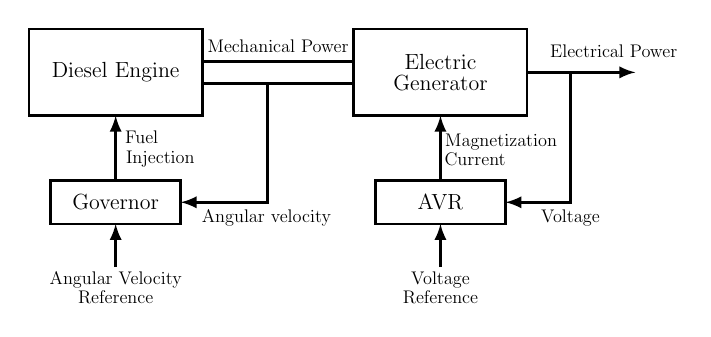
\begin{tikzpicture}[scale=0.55,transform shape]

 \node at (-1.5,1) {\Large{Diesel Engine}};
\draw  [-latex,line width=1pt](-3.5,2) rectangle (0.5,0);
\draw [-latex,line width=1pt] (4,2) rectangle (8,0);
\draw [line width=1pt](0.5,1.25) -- (4,1.25);
\draw [line width=1pt](0.5,0.75) -- (4,0.75);
 \node at (6,1.25) {\Large{Electric}};
 \node at (6,0.75) {\Large{Generator}};
 \node at (-1.5,-2) {\Large{Governor}};
 \node at (6,-2) {\Large{AVR}};
\draw  [-latex,line width=1pt](-3,-1.5) rectangle (0,-2.5);
\draw  [-latex,line width=1pt](4.5,-1.5) rectangle (7.5,-2.5);
\draw [-latex,line width=1pt](-1.5,-1.5) -- (-1.5,0);
\draw [-latex,line width=1pt](2,0.75) -- (2,-2) -- (0,-2);
\draw [-latex,line width=1pt](6,-1.5) -- (6,0);
\draw [-latex,line width=1pt](8,1) -- (10.5,1);
\draw [-latex,line width=1pt](9,1) -- (9,-2) -- (7.5,-2);
\node at (-0.9,-0.5) {\large{Fuel}};
\node at (-0.47,-1) {\large{Injection}};
\node at (2.25,1.6) {\large{Mechanical Power}};
\node at (1.98,-2.35) {\large{Angular velocity}};
\node at (9,-2.35) {\large{Voltage}};
\node at (10,1.5) {\large{Electrical  Power}};
\node at (7.4,-0.6) {\large{Magnetization}};
\node at (6.8,-1) {\large{Current}};
\draw  [-latex,line width=1pt](-1.5,-3.5) -- (-1.5,-2.5);
\draw  [-latex,line width=1pt](6,-3.5) -- (6,-2.5);
\node at (-1.5,-3.8) {\large{Angular Velocity}};
\node at (-1.5,-4.2) {\large{Reference}};
\node at (6,-3.8) {\large{Voltage}};
\node at (6,-4.2) {\large{Reference}};
\end{tikzpicture} 
%\end{figure}
\begin{itemize}
	\item<1->  
	\item<1-> Write something awesome!
	\begin{itemize}
		\item
	\end{itemize}
	\item<1-> 
\end{itemize}

\end{frame}


\begin{frame}{System decription}{System description}
\begin{itemize}
	\item<1-> 
\end{itemize}	
% \begin{figure}[H]
% \centering
% % This file was created by matlab2tikz.
%
%The latest updates can be retrieved from
%  http://www.mathworks.com/matlabcentral/fileexchange/22022-matlab2tikz-matlab2tikz
%where you can also make suggestions and rate matlab2tikz.
%
\definecolor{mycolor1}{rgb}{0.00000,0.44700,0.74100}%
%
\begin{tikzpicture}

\begin{axis}[%
width=0.75\columnwidth,
height=1.9in,
at={(0.758in,0.481in)},
scale only axis,
xmin=69,
xmax=72,
xlabel={Time [s]},
xmajorgrids,
ymin=30,
ymax=60,
ylabel={Power [kW]},
ymajorgrids,
axis background/.style={fill=white},
title style={font=\bfseries},
title={Genset}
]
\addplot [color=mycolor1,solid,forget plot]
  table[row sep=crcr]{%
69	42.0960090642869\\
69.00238	42.5559127479842\\
69.00448	36.9304035360587\\
69.00788	36.6986566116855\\
69.0092	41.9040380689165\\
69.01452	36.3199030238924\\
69.0198	42.7008963276288\\
69.02228	42.4192813188401\\
69.02452	37.0509363491857\\
69.02918	41.9996463688265\\
69.03454	36.3947483400785\\
69.03458	36.4410586652751\\
69.03918	42.7221469649957\\
69.04236	42.3933520014313\\
69.04792	36.6963423109946\\
69.0499	41.8899368936894\\
69.05454	36.4234595826002\\
69.05786	37.3699294333512\\
69.05916	42.6899957342084\\
69.06226	42.4038924677669\\
69.06788	36.6999047397127\\
69.07238	41.8721813488837\\
69.07456	36.2972837091461\\
69.0778	37.4358016851034\\
69.07922	42.7229193761768\\
69.0831	42.1095546802261\\
69.0879	36.6864335616395\\
69.09234	41.9090754786125\\
69.09454	36.3530078466834\\
69.09788	37.4736333563494\\
69.09924	42.803456752\\
69.10788	36.8654118284957\\
69.1092	42.053927176649\\
69.11236	41.8526943259543\\
69.1146	36.487117478319\\
69.11916	42.8016329754773\\
69.12444	37.1177209561857\\
69.12794	36.79171310045\\
69.12988	42.0205814942576\\
69.1324	41.954159768411\\
69.13454	36.5077477883357\\
69.13922	42.8079391245626\\
69.14452	37.0621687492813\\
69.14788	36.8206470621655\\
69.14924	41.9535676146947\\
69.15454	36.4610679948756\\
69.159	42.6757066554406\\
69.1592	42.9818657293557\\
69.16448	37.0721743774901\\
69.16792	36.786152688155\\
69.1724	42.0061495743427\\
69.17454	36.4569230249899\\
69.1792	42.915073892547\\
69.17978	42.8051384911361\\
69.18446	37.1797525446474\\
69.18794	36.9837290386078\\
69.1892	42.1755218118723\\
69.19458	36.5808635386711\\
69.1992	42.8726922139985\\
69.20236	42.5029991764865\\
69.2045	36.9679436405511\\
69.2079	36.7118718139959\\
69.20916	42.0321879179646\\
69.21454	36.4941907596754\\
69.21976	42.8314160043567\\
69.22228	42.5236552886485\\
69.22794	36.8211016657531\\
69.23232	41.9880176153725\\
69.23456	36.3773625124651\\
69.23784	37.5166323154776\\
69.23916	42.8174871562231\\
69.24232	42.590353934823\\
69.24788	36.7503466947837\\
69.25226	41.9948603146254\\
69.25454	36.4288644289047\\
69.25782	37.5208282942826\\
69.25912	42.8203444510937\\
69.26304	42.110040536459\\
69.26786	36.824783134485\\
69.26978	41.9860289022677\\
69.27454	36.4985082200892\\
69.2778	37.388844183683\\
69.27912	42.8050592828384\\
69.2879	36.7534873638932\\
69.28916	41.9644014044407\\
69.29228	41.8569769949865\\
69.2945	36.4587110791705\\
69.29784	37.4018825436509\\
69.29912	42.7001597566365\\
69.30786	36.7372144598477\\
69.30912	41.8394833021144\\
69.31232	41.9174742451826\\
69.31446	36.407544666765\\
69.31914	42.77189820798\\
69.32448	36.8780068976299\\
69.32786	36.6577634656352\\
69.3298	41.8818526132918\\
69.33238	41.9412082546322\\
69.33452	36.3830499324044\\
69.3391	42.7921672914878\\
69.34446	37.0097091863565\\
69.34788	36.8212195523597\\
69.34918	42.0316253352224\\
69.35446	36.5085142398206\\
69.35914	42.8028840999977\\
69.35978	42.7308984749884\\
69.36446	36.8317367049195\\
69.36784	36.6425410625091\\
69.36986	41.93765235963\\
69.37454	36.4997869016355\\
69.37918	42.7663234961048\\
69.3823	42.4607232735905\\
69.38446	36.9269220451554\\
69.3879	36.7404906274645\\
69.39238	41.9457678173549\\
69.39452	36.4035279290206\\
69.39916	42.8613109897251\\
69.40236	42.5040022099868\\
69.40782	36.6954435348295\\
69.41236	41.9242553436566\\
69.41452	36.4317646157955\\
69.41476	37.0588116662464\\
69.41918	42.8055489910929\\
69.42226	42.4343695662523\\
69.42788	36.8109381920963\\
69.42922	41.9893380110246\\
69.43456	36.5288328574307\\
69.4378	37.4111151810318\\
69.43914	42.8096294189846\\
69.4424	42.2350981400335\\
69.44794	36.6461690103002\\
69.4499	41.979658643863\\
69.45452	36.6182238286659\\
69.4578	37.5080650981595\\
69.45918	42.8559135535829\\
69.46314	42.0411276929031\\
69.46788	36.7851028227498\\
69.47226	42.118916774762\\
69.47454	36.5688613736583\\
69.4778	37.6250868880573\\
69.47918	42.9697407046519\\
69.48794	36.7646662185471\\
69.48986	42.0351962137481\\
69.49236	42.0361810071846\\
69.49454	36.5193737098206\\
69.49916	42.8620786088031\\
69.50446	37.0578649575612\\
69.50788	36.7793626852272\\
69.50922	42.0225589214941\\
69.51238	41.8944825193229\\
69.5145	36.5327212654563\\
69.51912	42.8688581051802\\
69.52444	36.8543179818252\\
69.5279	36.6547344981785\\
69.52916	41.9774191997382\\
69.53456	36.6068834346194\\
69.53916	42.7941129209847\\
69.53974	42.7837982394699\\
69.54452	36.9256417413792\\
69.5479	36.7050533784797\\
69.55232	42.0417907518976\\
69.55454	36.4637929455961\\
69.55914	42.895415486223\\
69.56236	42.5572723675891\\
69.5645	36.8584055010284\\
69.56784	36.6438912346442\\
69.57236	41.9988491640251\\
69.57452	36.5215951636116\\
69.57912	42.9030254298698\\
69.58226	42.4721688147962\\
69.58448	37.034132909233\\
69.5892	42.0190249373194\\
69.59446	36.6333491906225\\
69.59452	36.5982302821719\\
69.59914	42.8737160126058\\
69.60234	42.4063261330556\\
69.60786	36.6724513371134\\
69.61236	41.9903464607732\\
69.61454	36.6102046278257\\
69.61774	37.5731619716849\\
69.61918	42.8226545773196\\
69.62226	42.4460644797842\\
69.62786	36.7232732693329\\
69.63226	42.0212667813456\\
69.63452	36.4991020600841\\
69.6378	37.5741224595183\\
69.63908	42.8657702982625\\
69.64308	42.1533547120755\\
69.64784	36.7065393692507\\
69.65226	41.9918094850021\\
69.6545	36.4806024986324\\
69.65776	37.5760328326756\\
69.65916	42.8587972534398\\
69.6678	36.8337109058741\\
69.66914	42.0196817592662\\
69.67226	41.9535243730622\\
69.67452	36.5865079747009\\
69.67908	42.8851210679419\\
69.68434	37.0164445499283\\
69.68784	36.6608366574602\\
69.68984	41.9880457954753\\
69.69236	41.8906351024035\\
69.69446	36.6019866596949\\
69.69912	42.8403754795681\\
69.70444	37.0022050329855\\
69.70786	36.7768392610297\\
69.70914	41.9176533135105\\
69.71448	36.4810131862259\\
69.7189	42.4050407810376\\
69.71908	42.8068381370481\\
69.72444	36.9350586779022\\
69.72788	36.7373228123708\\
69.73222	41.9812202700803\\
69.73452	36.4482173644258\\
69.73914	42.8121520067398\\
69.73972	42.7135639428442\\
69.74444	37.0044698724979\\
69.74782	36.7570272666854\\
69.74916	41.9263731958314\\
69.75448	36.4305931426707\\
69.75908	42.7642749899312\\
69.7623	42.329544517957\\
69.76446	36.8039268639819\\
69.76782	36.6717828391125\\
69.76916	41.8965328448592\\
69.7745	36.4979571222339\\
69.77912	42.6639264703874\\
69.78226	42.3699744944883\\
69.78786	36.6961571853764\\
69.7923	41.8776065753919\\
69.79452	36.364257480237\\
69.79778	37.4123091368669\\
69.79914	42.714239762884\\
69.80234	42.5033927383611\\
69.80782	36.6428529438385\\
69.81224	41.8693333666181\\
69.8145	36.303175864263\\
69.81774	37.4123313761866\\
69.81916	42.7569423768142\\
69.82302	42.0705679621064\\
69.82782	36.7724567682369\\
69.82976	41.9534202542857\\
69.83448	36.455942944107\\
69.83772	37.3257198163572\\
69.8391	42.7341242785117\\
69.84786	36.6695134425217\\
69.84974	41.9192503473183\\
69.85228	41.8234992149201\\
69.85448	36.4379300577773\\
69.85778	37.3533376711531\\
69.85916	42.6520996667939\\
69.8678	36.7561284869509\\
69.86914	41.8756984544379\\
69.8723	41.8753398842983\\
69.87448	36.2689492537303\\
69.87906	42.673723185013\\
69.88444	36.9482302550381\\
69.88782	36.6794774124858\\
69.88978	41.8730640727767\\
69.89226	41.8227102790494\\
69.89446	36.299687826756\\
69.8991	42.6791835505121\\
69.90444	37.0054999908332\\
69.90782	36.7685965083308\\
69.90916	41.9177155668194\\
69.91446	36.3318083734199\\
69.9191	42.7692211022521\\
69.91974	42.6682597928314\\
69.92444	36.9583777985286\\
69.92782	36.7610511912757\\
69.92916	41.9777344976742\\
69.93444	36.4694139772641\\
69.93972	42.7071721658007\\
69.94226	42.5203160639268\\
69.9444	37.040660311027\\
69.94782	36.8009511791569\\
69.95236	41.9439478633753\\
69.95452	36.3533483033263\\
69.95914	42.8359017849269\\
69.96234	42.6233830320923\\
69.96776	36.8665328345388\\
69.96984	41.8724544675611\\
69.97448	36.3520956009231\\
69.97468	36.8060974517473\\
69.97912	42.8304582964292\\
69.98228	42.5371843267494\\
69.98782	36.8442465988498\\
69.9891	41.9757908000066\\
69.99448	36.3964010888729\\
69.9978	37.4176116882202\\
69.99908	42.8177555747184\\
70.00232	42.484527445938\\
70.00786	36.7113305992732\\
70.00984	41.8856763746872\\
70.0145	36.4156829239612\\
70.01782	37.3991650847187\\
70.0197	42.7336589990408\\
70.02314	42.0755950250889\\
70.02782	36.7151396052684\\
70.03228	41.8643233127954\\
70.03452	36.2389573116088\\
70.03778	37.3723718319427\\
70.03912	42.7285120506424\\
70.04788	36.6496405318085\\
70.04914	41.793721201515\\
70.0523	41.7963466234005\\
70.05452	36.2534007846297\\
70.05918	42.7783813058802\\
70.06444	37.0672784807627\\
70.0679	36.765071488122\\
70.06918	41.901030034585\\
70.07228	41.6752178202025\\
70.07454	36.2889092215104\\
70.07918	42.7296110069536\\
70.08444	36.9184431859163\\
70.08788	36.6537777013455\\
70.08922	41.8198808324584\\
70.0945	36.3479600766345\\
70.0991	42.7096092634951\\
70.10446	36.9846087586051\\
70.10782	36.7112646769021\\
70.1123	41.8483568369744\\
70.11456	36.2573770911153\\
70.11914	42.7770127146621\\
70.1223	42.6296559544271\\
70.12448	36.9821079937539\\
70.12788	36.6300343687272\\
70.12982	41.7976287282342\\
70.13454	36.2420937164587\\
70.13916	42.7871454197887\\
70.1423	42.533514984814\\
70.14442	37.1082496000103\\
70.14912	41.9265248766925\\
70.1544	36.4299458695279\\
70.15444	36.3175826285389\\
70.1591	42.75221349622\\
70.16232	42.4511792064021\\
70.16786	36.6731747832976\\
70.16914	41.8915582455588\\
70.17448	36.4204421342659\\
70.17776	37.4405341217313\\
70.17916	42.8228488278424\\
70.18226	42.5801851776344\\
70.18784	36.7604632167825\\
70.1923	41.9403646247269\\
70.19454	36.3555067638187\\
70.19776	37.5714972191957\\
70.1991	42.8752468482219\\
70.20312	42.292661758565\\
70.20788	36.7628987651489\\
70.2098	41.900182952876\\
70.21446	36.3630673153674\\
70.21776	37.5400264214233\\
70.21914	42.9327582937706\\
70.2278	36.8665092742814\\
70.22916	42.0076093979571\\
70.23224	41.7879450409198\\
70.23446	36.4638425430387\\
70.2391	42.9061895585622\\
70.24426	37.3739368537502\\
70.24784	36.756891812381\\
70.24914	41.9703978986432\\
70.25236	41.8643394481613\\
70.25452	36.4757961823336\\
70.25914	42.8340255801467\\
70.26444	37.0901425588157\\
70.26712	33.4333518715314\\
70.2701	51.0612878172907\\
70.27442	45.0270296557091\\
70.27682	52.0299781725829\\
70.27996	52.6370796498976\\
70.28452	45.4213424162415\\
70.28794	44.6237789459264\\
70.29016	51.415011874031\\
70.29466	44.3580493103096\\
70.29936	51.5584043448115\\
70.29996	52.3206350845798\\
70.30472	44.8785884544262\\
70.30814	44.041840018107\\
70.31022	50.7605625085435\\
70.31492	43.6763221523153\\
70.32018	51.5075105455175\\
70.32032	51.3829253849544\\
70.32496	44.0128361249953\\
70.32838	43.3254468917184\\
70.3305	50.0694149513089\\
70.33518	43.1232268968911\\
70.34042	50.9410201240271\\
70.34392	50.3253953211744\\
70.34524	43.6762499398367\\
70.34868	43.1052248172896\\
70.35084	49.5799595597726\\
70.3555	42.8578169457409\\
70.36076	50.7819782570496\\
70.36432	50.4067160630674\\
70.36556	43.606190474468\\
70.3691	43.1134425602216\\
70.37114	49.7741295280009\\
70.37582	43.0844331900038\\
70.38116	51.1493496309611\\
70.38466	50.7323737407894\\
70.38942	43.6363414286325\\
70.38948	43.5610609514674\\
70.39156	50.2168431668401\\
70.39634	43.9556051350353\\
70.40168	51.8677379148232\\
70.40512	51.2971696856992\\
70.4099	44.0849771804608\\
70.41016	44.6863176272748\\
70.41538	51.1031476588399\\
70.42012	45.7436161754844\\
70.4221	52.7617468270531\\
70.4256	52.051468648218\\
70.43046	44.6920663529853\\
70.43584	51.7687343198908\\
70.43722	45.1753983882474\\
70.4406	46.4681780780348\\
70.44264	53.3524229498904\\
70.44614	52.8463425475193\\
70.45096	45.297907407443\\
70.45644	52.5797504900231\\
70.4578	45.7513244890023\\
70.4612	47.0941907068898\\
70.46318	53.9448211026162\\
70.46664	53.3498162768413\\
70.4715	45.7905099944217\\
70.47696	52.9290799038313\\
70.4783	46.1417471975033\\
70.48176	47.1715338491421\\
70.48376	54.3076377929939\\
70.48732	53.3087210867324\\
70.49214	45.7036512918599\\
70.49754	53.0939652307264\\
70.49894	46.4921270408411\\
70.50234	47.3220693284716\\
70.50434	54.5801847824257\\
70.50784	53.5357680014059\\
70.51268	45.9817782959345\\
70.51814	53.1780776438423\\
70.51954	46.3042209255278\\
70.52296	47.557876400469\\
70.52496	54.5104504956446\\
70.52842	53.8084588406305\\
70.53334	46.0505475641449\\
70.53878	53.474135757836\\
70.54016	46.3291178845373\\
70.54554	54.5761580493906\\
70.54702	47.6685151766476\\
70.54906	53.9946394665389\\
70.55394	46.2765422060897\\
70.5593	53.4605161624306\\
70.56076	46.5471472561103\\
70.56616	54.7370809573415\\
70.5676	47.5242556654587\\
70.56964	53.7100069786024\\
70.57452	46.048206073811\\
70.5799	53.3642183835991\\
70.58136	46.5870739632439\\
70.58474	47.3738460134918\\
70.58676	54.7811459105041\\
70.5902	53.5741387458698\\
70.59512	46.0162184950858\\
70.60044	53.2689257670258\\
70.60192	46.3407001039976\\
70.60526	47.4838924597703\\
70.6073	54.4591865949604\\
70.61076	53.728757906489\\
70.61564	45.995902235353\\
70.62248	46.2101188146408\\
70.62442	53.4178719597936\\
70.62776	54.4665928610968\\
70.6293	47.4830182607215\\
70.63138	53.7553171972382\\
70.63614	46.1953934157764\\
70.64156	53.4171777168288\\
70.643	46.4713864214292\\
70.64636	47.3768712027847\\
70.64832	54.6002975744565\\
70.65666	45.8569787963197\\
70.65884	53.1335981567439\\
70.66344	46.458594163468\\
70.6654	53.3697027612792\\
70.66686	47.2460673257569\\
70.66878	54.6142378771633\\
70.67714	45.9288887794314\\
70.67916	52.9213374657093\\
70.68394	46.1384706541846\\
70.68598	53.4896855512499\\
70.6873	47.3767854949597\\
70.68922	54.3032857271693\\
70.69754	45.9856948182314\\
70.69968	52.7660264259117\\
70.7029	53.4712901047816\\
70.70436	46.1638417997717\\
70.7097	54.4434781959212\\
70.7143	47.2733834995909\\
70.71794	46.0634317883033\\
70.71994	53.0916339012504\\
70.72332	53.183397416083\\
70.72472	46.3679717648648\\
70.73006	54.6456812078542\\
70.73486	46.6017512488447\\
70.73832	45.7060870112994\\
70.74036	53.059097481874\\
70.74506	46.2518721969053\\
70.7471	53.3391132704582\\
70.75038	54.361081973192\\
70.75524	46.3817388956859\\
70.75864	45.7970685573912\\
70.76066	52.6545703831312\\
70.7654	45.9109058804537\\
70.76742	53.2095452892685\\
70.77068	54.1948604126283\\
70.77548	46.3621983123932\\
70.77896	45.7759002862416\\
70.78094	52.6828063269633\\
70.78568	46.0245537717798\\
70.79034	53.7257682896201\\
70.79088	54.3422643429994\\
70.79576	46.578120088384\\
70.79922	45.8312285475219\\
70.80118	52.9070097043879\\
70.80596	46.163135245419\\
70.81108	54.1259960074531\\
70.81118	54.3399655847597\\
70.81594	46.370086974186\\
70.81938	45.7072377065637\\
70.82474	52.9720049111994\\
70.8261	46.0348100332574\\
70.83136	54.2607443313268\\
70.83476	53.4765411760567\\
70.83612	46.3409434972265\\
70.83962	45.6858143360648\\
70.84484	52.8878387832955\\
70.8463	45.821731262282\\
70.8515	54.0868203392586\\
70.85496	53.4425537299104\\
70.85622	46.2893706910563\\
70.85974	45.5612079733088\\
70.86498	52.8882747486843\\
70.86644	45.7693331176533\\
70.8716	54.1204405474887\\
70.87504	53.4006889979986\\
70.8798	45.7267285306345\\
70.88506	52.8151350209591\\
70.88646	45.8803454051915\\
70.88976	46.8893219738248\\
70.89172	54.1289831019751\\
70.89522	53.2125391039367\\
70.89984	45.5363517421172\\
70.902	52.8752164079188\\
70.90658	45.8760425090686\\
70.90982	46.8630037113443\\
70.91176	53.9865188452069\\
70.91512	53.1723407594623\\
70.9199	45.5343328152526\\
70.9266	45.6081575584656\\
70.9286	52.8111042707701\\
70.92984	46.9075678156745\\
70.93178	53.8425325440476\\
70.9355	52.8444890512657\\
70.93996	45.4385480618212\\
70.94656	45.6980239149082\\
70.94872	52.8882699966355\\
70.94984	46.9055728687006\\
70.95174	53.9704814822403\\
70.95994	45.6019429247602\\
70.96206	52.7520019525097\\
70.96656	45.7251724898296\\
70.96866	52.8450416537913\\
70.97172	53.9029444009135\\
70.97648	46.0945817472229\\
70.97988	45.4944010977029\\
70.98204	52.7986397507548\\
70.9865	45.7987218283703\\
70.98858	52.8380118482897\\
70.99168	53.8662395758284\\
70.99648	46.1781583892232\\
70.99986	45.4871108204855\\
71.00196	52.5812407753444\\
71.00652	45.6119390277517\\
71.01154	53.5642499406528\\
71.01166	53.8755023989569\\
71.01638	46.1930321984351\\
71.01978	45.5102786457739\\
71.02506	52.7751795374079\\
71.02644	45.666844549586\\
71.03162	53.8204830261127\\
71.035	53.2166341297505\\
71.03636	46.2295441526076\\
71.03976	45.5867395357371\\
71.04184	52.6738603948888\\
71.04638	45.650931677116\\
71.0516	53.8317166394311\\
71.05504	53.0551145567429\\
71.05966	45.4552626139033\\
71.06184	52.8988746667906\\
71.06632	45.702507006692\\
71.06958	46.6774869894146\\
71.0715	53.7784324843029\\
71.07494	53.0653782256745\\
71.07964	45.4515267155651\\
71.08484	52.5988589124266\\
71.08626	45.5598736672088\\
71.08948	46.7900686135001\\
71.09136	53.7262798437442\\
71.09486	53.3126747061282\\
71.09956	45.4126530847545\\
71.10618	45.5812691548811\\
71.10826	52.8313134363347\\
71.10942	46.7704094006248\\
71.1114	53.775489125655\\
71.11942	45.5805132050611\\
71.12148	52.7039878462102\\
71.1261	45.6762864177441\\
71.12826	52.7666402185948\\
71.13126	53.8183865067846\\
71.13594	46.1676705503499\\
71.13934	45.4510834156985\\
71.14148	52.8505507288321\\
71.14598	45.7880589007258\\
71.14812	52.8728054102785\\
71.15114	53.8554514106023\\
71.1559	46.1890533353317\\
71.15928	45.4875206927114\\
71.16144	52.6010246977267\\
71.16592	45.6383539910224\\
71.17054	53.1326230870118\\
71.17112	53.8298457471931\\
71.1758	46.2639093163582\\
71.1792	45.5457551969846\\
71.18138	52.7703770438821\\
71.18584	45.7619325017938\\
71.19104	53.9710059911579\\
71.19126	53.6005547822995\\
71.19568	46.328592518036\\
71.19916	45.6422609399174\\
71.2011	52.7916659502918\\
71.20574	45.7495074352876\\
71.21092	53.8242368660776\\
71.21434	53.1105267545364\\
71.21892	45.8014730331351\\
71.21906	45.5375154027807\\
71.22122	52.8863051217464\\
71.22584	46.1162649437828\\
71.23082	53.7847107447256\\
71.23424	52.9998205496609\\
71.23902	45.4215595723371\\
71.24416	52.5778840397923\\
71.24564	45.5963351028877\\
71.25076	53.7523653072162\\
71.25226	46.8153623547406\\
71.25428	53.228351465265\\
71.25888	45.4089775335227\\
71.26416	52.7226505906436\\
71.26552	45.5804281443879\\
71.26878	46.8440569700461\\
71.27068	53.7983085410215\\
71.27422	53.1670421717814\\
71.27878	45.5776362640795\\
71.28542	45.697043742227\\
71.2876	52.7739070520813\\
71.28872	46.7123560619483\\
71.29066	53.8404692782426\\
71.2987	45.455341253429\\
71.30082	52.967622311168\\
71.30534	45.8341020324545\\
71.3075	53.0162246513311\\
71.31054	53.9218924139003\\
71.31522	46.2004990300383\\
71.31864	45.5837536934881\\
71.32078	52.7494812496192\\
71.3253	45.7367725811661\\
71.32728	53.0100687352494\\
71.33046	53.8583271865866\\
71.33514	46.1856147666826\\
71.33854	45.4951831614787\\
71.34076	52.809506645643\\
71.3452	45.739567552735\\
71.35026	53.74352230674\\
71.35034	53.9433276684657\\
71.35506	46.236207372945\\
71.35848	45.653496394306\\
71.36062	52.7951805276131\\
71.36512	45.7759925223722\\
71.37026	53.8794699046798\\
71.37376	53.1044121280087\\
71.37498	46.0806476844957\\
71.37844	45.4868144744202\\
71.38058	52.9282167531453\\
71.38502	45.8503500080722\\
71.39028	53.7718272174376\\
71.39366	53.0253042356665\\
71.39838	45.4594464350904\\
71.40354	52.6916534151757\\
71.40502	45.6852258456259\\
71.4102	53.7071814641592\\
71.4116	46.8211955279325\\
71.41358	53.2477445173588\\
71.41832	45.3907465967294\\
71.4235	52.7373899113007\\
71.42494	45.6889670158353\\
71.43008	53.7636343634088\\
71.43158	46.8197989979884\\
71.43352	53.1012451632762\\
71.43824	45.5120156820241\\
71.4449	45.7741150182542\\
71.44686	52.8660004480151\\
71.44816	46.788708962806\\
71.45008	53.8548757857459\\
71.45822	45.3392168913569\\
71.46038	52.8192970747851\\
71.46482	45.8215205009855\\
71.46696	52.9485101794179\\
71.47004	53.8307051121251\\
71.47468	46.0800369319881\\
71.47818	45.3470706526821\\
71.48038	52.5090702706056\\
71.48484	45.7550091254727\\
71.48692	53.011094034409\\
71.49004	53.7751845303762\\
71.49476	46.0171126873648\\
71.4981	45.345935350152\\
71.50032	52.6876271171174\\
71.50478	45.8388496800331\\
71.50694	53.0939826428947\\
71.50996	53.9490689864845\\
71.51466	46.2266381174789\\
71.5181	45.598964319369\\
71.52022	52.8251470352419\\
71.5248	45.9630681901844\\
71.52994	53.975312020931\\
71.52998	53.9192777078161\\
71.53464	46.0658678056462\\
71.5381	45.4759350071745\\
71.54024	52.9278236844977\\
71.54476	45.9469327005668\\
71.54998	53.9781367845431\\
71.55334	53.0216023359351\\
71.55464	46.0672247166272\\
71.55806	45.4302100667347\\
71.56332	52.7960673500643\\
71.5647	45.7884692867009\\
71.5699	53.8735089682672\\
71.57342	53.2626210893572\\
71.57808	45.3630081685931\\
71.58328	52.7973478406942\\
71.58472	45.7446393374658\\
71.5899	53.85229132014\\
71.5914	46.8677891739702\\
71.59332	53.0964144548605\\
71.59808	45.4913139733374\\
71.6033	52.6933883883415\\
71.60474	45.8076804813001\\
71.60994	53.8726274516012\\
71.61144	46.7863236137181\\
71.61334	52.8617153136903\\
71.61806	45.3502748719974\\
71.62468	45.9635046382304\\
71.62668	53.0382351511764\\
71.628	46.9089211281453\\
71.6299	53.9494289280146\\
71.63804	45.461042109999\\
71.6402	52.6431118216925\\
71.64474	45.8141150403477\\
71.6468	53.1759775123072\\
71.64996	53.883022460981\\
71.6514	46.8879095506741\\
71.65804	45.4463659609614\\
71.66018	52.7264287046177\\
71.6647	45.8599489824402\\
71.66692	53.1242565937357\\
71.66998	53.979935575924\\
71.67466	46.1881184604331\\
71.6781	45.55271791248\\
71.68014	52.7041392725163\\
71.68468	45.8762577926624\\
71.6869	52.9409578377688\\
71.68994	53.9523136969509\\
71.69466	46.0751005557795\\
71.6981	45.4371906940874\\
71.70028	52.8665951301647\\
71.70474	45.9454504243325\\
71.70942	53.1604039981791\\
71.70992	53.9223473031121\\
71.7147	46.0774081679726\\
71.71806	45.4407000625245\\
71.72336	52.7221376039639\\
71.72476	45.7302012615513\\
71.73004	53.8099730197797\\
71.7334	53.2686401201852\\
71.73472	46.0269367833876\\
71.73812	45.4335099851671\\
71.74346	52.7873092892084\\
71.7448	45.7293354849006\\
71.75	53.9497010490111\\
71.75348	53.231161124839\\
71.7581	45.62922828975\\
71.75814	45.5335702763121\\
71.76026	52.7145111114315\\
71.765	46.2451881997123\\
71.77002	53.9196814621306\\
71.77342	53.0470056053912\\
71.77818	45.4631350951541\\
71.78036	52.8110711129915\\
71.78488	45.8701628601327\\
71.78818	46.8923014426777\\
71.79008	53.9322144290508\\
71.79348	53.1432967423413\\
71.79818	45.4671469355143\\
71.80346	52.7225432075655\\
71.80488	45.7318839286489\\
71.81008	53.8194148640969\\
71.81162	46.9350148922799\\
71.81358	53.2514693485467\\
71.81824	45.391950731599\\
71.82492	45.7622832016656\\
71.82712	52.9400956973315\\
71.8301	53.8441171992288\\
71.83156	46.8356171323209\\
71.8383	45.526069851479\\
71.8404	52.6324168520036\\
71.84496	45.7895375075205\\
71.84706	52.8336770337942\\
71.85014	53.8649545795265\\
71.85484	46.0582027818685\\
71.85828	45.4302086542731\\
71.86046	52.8107412541967\\
71.86496	45.8001400185275\\
71.86696	52.874324180956\\
71.8702	53.8047196522671\\
71.87492	46.0321149627677\\
71.87832	45.4081487450516\\
71.88038	52.4780615101239\\
71.88494	45.6927567221298\\
71.8871	52.938330651442\\
71.89022	53.7600860257251\\
71.89496	46.1237513000333\\
71.89834	45.3899405502807\\
71.9005	52.6137415783747\\
71.90496	45.7476822300895\\
71.91016	53.8464769291072\\
71.9102	53.8929121342285\\
71.91496	46.2344067936436\\
71.91834	45.5359331500602\\
71.92362	52.7188728994013\\
71.925	45.8253860071405\\
71.93022	53.8543965895169\\
71.93376	52.9999268539752\\
71.93496	46.0157395135321\\
71.93838	45.4109499564233\\
71.94054	52.8117236847835\\
71.94502	45.8907996647965\\
71.9503	53.8903208988447\\
71.95372	53.113645385727\\
71.9584	45.4687743282712\\
71.96366	52.6676916031822\\
71.96506	45.6776161737613\\
71.96834	46.8777312225649\\
71.97026	53.8569326329298\\
71.97378	53.3118080674071\\
71.97844	45.4383063290145\\
71.98362	52.8455554249023\\
71.98502	45.7419538949208\\
71.98834	46.9331212412499\\
71.9903	53.9297977549192\\
72.00002	51.7077566657693\\
};
\end{axis}
\end{tikzpicture}% 
% \end{figure}
\end{frame}

\subsection{System description}

\begin{frame}{System decription}{System description}
\begin{itemize}
	\item<1->    
	\item<1->    
\end{itemize}
% \begin{figure}[H]
% \centering
% % This file was created by matlab2tikz.
%
%The latest updates can be retrieved from
%  http://www.mathworks.com/matlabcentral/fileexchange/22022-matlab2tikz-matlab2tikz
%where you can also make suggestions and rate matlab2tikz.
%
\definecolor{mycolor1}{rgb}{0.00000,0.44700,0.74100}%
%
\begin{tikzpicture}
\begin{axis}[%
{width=0.75\columnwidth},
height=1.7in,
at={(0.758in,0.481in)},
scale only axis,
xmin=10,
xmax=20,
xlabel={Time [s]},
xmajorgrids,
ymin=-1,
ymax=11,
ylabel={Power [kW]},
ymajorgrids,
axis background/.style={fill=white},
title style={font=\bfseries},
ytick={0, 2, 4, 6, 8, 10},
title={Inverter}
]
\addplot [color=mycolor1,solid,forget plot]
  table[row sep=crcr]{%
9.997	0\\
10.067	0\\
10.138	0\\
10.218	0\\
10.278	0\\
10.348	0\\
10.431	0\\
10.508	0\\
10.578	0\\
10.633	0\\
10.708	0\\
10.778	0\\
10.848	0\\
10.932	0\\
10.998	0\\
11.088	0\\
11.178	0\\
11.198	0\\
11.288	0\\
11.332	0.1\\
11.408	0.1\\
11.478	0.1\\
11.548	0\\
11.632	0\\
11.708	0\\
11.778	0\\
11.831	0\\
11.909	0\\
11.979	0\\
12.049	0\\
12.131	0\\
12.209	0\\
12.279	0\\
12.332	0\\
12.409	0\\
12.48	0\\
12.55	0\\
12.651	0\\
12.71	0.1\\
12.751	0.1\\
12.834	0.1\\
12.912	0\\
12.992	0\\
13.036	0\\
13.112	0\\
13.193	0\\
13.236	0\\
13.313	0\\
13.383	0\\
13.454	0\\
13.537	0\\
13.614	0.4\\
13.684	0.4\\
13.737	1.1\\
13.814	1.1\\
13.895	1.1\\
13.939	1.7\\
14.015	1.7\\
14.085	2.4\\
14.155	2.4\\
14.238	2.4\\
14.316	3.2\\
14.385	3.8\\
14.455	3.8\\
14.539	3.8\\
14.616	4.5\\
14.685	5.3\\
14.739	5.3\\
14.816	5.3\\
14.885	5.3\\
15.006	5.9\\
15.015	5.9\\
15.085	5.9\\
15.155	6.6\\
15.238	6.6\\
15.315	7.3\\
15.385	7.3\\
15.455	7.3\\
15.542	8\\
15.643	8.7\\
15.686	8.7\\
15.739	8.7\\
15.816	8.7\\
15.886	9.5\\
15.956	9.5\\
16.041	10\\
16.116	10\\
16.186	10.1\\
16.239	10.1\\
16.316	10.1\\
16.386	10.1\\
16.457	10.1\\
16.54	10.1\\
16.617	10.1\\
16.687	10.2\\
16.757	10.2\\
16.842	10.2\\
16.917	10.1\\
16.987	10.1\\
17.057	10.1\\
17.145	10.1\\
17.187	10.1\\
17.257	10.1\\
17.343	10.1\\
17.418	10.1\\
17.488	10.1\\
17.558	10\\
17.608	10\\
17.689	10.1\\
17.742	10.1\\
17.819	10.1\\
17.889	10.2\\
17.969	10.2\\
18.019	10.1\\
18.089	10.1\\
18.159	10.1\\
18.242	10.1\\
18.32	10.1\\
18.39	10.2\\
18.46	10.2\\
18.543	10.2\\
18.69	10.2\\
18.72	10.2\\
18.791	10.2\\
18.861	10.2\\
18.943	10.1\\
19.021	10.1\\
19.081	10.1\\
19.152	10.1\\
19.232	10.1\\
19.292	10.1\\
19.361	10.1\\
19.444	10.1\\
19.522	10.1\\
19.592	10.1\\
19.644	10.1\\
19.722	10.1\\
19.792	10.1\\
19.846	10.2\\
19.923	10.2\\
19.993	10\\
20.064	10\\
};
\end{axis}
\end{tikzpicture}% 
% \end{figure}
\end{frame}








%%%%%%%%%%%%%%%%
\section{Optimization}
%%%%%%%%%%%% MID WAY AGENDA %%%%%%%%%%%%%%
%\begin{frame}<beamer>
%\frametitle{Simon Bjerre Krogh}
%\tableofcontents[currentsection]
%\end{frame}


% the license


\begin{frame}{Optimization}{}
\begin{itemize}
	\item<1-> 
	\item<1-> Write something awesome!
	\begin{itemize}
		\item<1-> 
	\end{itemize}
	\item<1->  Write something awesome!
	\begin{itemize}
		\item<1-> 
		\item<1-> 
	\end{itemize}
\end{itemize}
% \begin{figure}[H]
% \centering
% 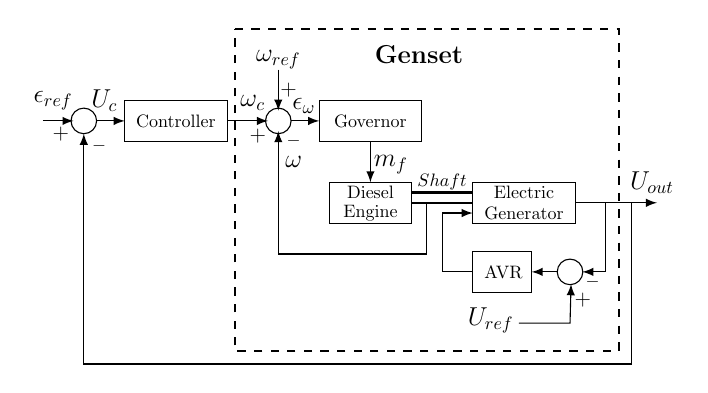
\begin{tikzpicture}[scale=0.65,transform shape]
\definecolor{mycolor1}{rgb}{0.00000,0.44700,0.74100}
\node at (2.95,1.5) {\Large{\textbf{Genset}}};
\node at (2,0.2) {\normalsize{Governor}};
\draw [-latex ] (1,0.6) rectangle (3,-0.2);
 \node at (2,-1.2) {\normalsize{Diesel}};
  \node at (2,-1.6) {\normalsize{Engine}};
\draw [-latex ] (1.2,-1) rectangle (2.8,-1.8);
\draw [-latex ](2,-0.2) -- (2,-1);
\node at (2.4,-0.65) {\Large{$m_f$}};
 \node at (5,-1.2) {\normalsize{Electric}};
  \node at (5,-1.6) {\normalsize{Generator}};
\draw [-latex ] (4,-1) rectangle (6,-1.8);

\node at (3.4,-1) {$Shaft$};
  \node at (4.6,-2.75) {\normalsize{AVR}};
\draw [-latex ] (5.9,-2.75) ellipse (0.25 and 0.25);
\draw [-latex ] (4,-2.35) rectangle (5.15,-3.15);
\draw [-latex ](4,-2.75) -- (3.4,-2.75) -- (3.4,-1.6) -- (4,-1.6);
\node at (6.34,-2.95) {$-$};
\draw [-latex ](4.9,-3.75) -- (5.9,-3.75) -- (5.92,-2.99);
\node at (4.35,-3.7) {\Large{$U_{ref}$}};
\node at (7.5,-1) {\Large{$U_{out}$}};
\draw [-latex ] (0.2,0.2) ellipse (0.25 and 0.25);

\draw [-latex ](0.2,1.2) -- (0.2,0.4);
\node at (0.2,1.4) {\Large{$\omega_{ref}$}};
\draw [-latex ](3.1,-1.4) -- (3.1,-2.4) -- (0.2,-2.4) -- (0.2,0);
\draw [dashed, thick](-0.65,2) -- (6.85,2) -- (6.85,-4.3) -- (-0.65,-4.3) -- (-0.65,2);
\node at (0.5,-0.6) {\Large{$\omega$}};
\node at (-1.8,0.2) {\normalsize{Controller}};
\draw [-latex ] (-2.8,0.6) rectangle (-0.8,-0.2);
\draw [-latex ](-0.8,0.2) -- (0,0.2);
\node at (-0.3,0.55) {\Large{$\omega_{c}$}};
\draw [-latex ] (-3.6,0.2) ellipse (0.25 and 0.25);
\draw [-latex ](-3.35,0.2) -- (-2.8,0.2);
\node at (-3.2,0.6) {\Large{$U_{c}$}};
\draw [-latex ](-4.4,0.2) -- (-3.8,0.2);
\node at (-4.2,0.6) {\Large{$\epsilon_{ref}$}};
\draw [-latex ](7.1,-1.4) -- (7.1,-4.55) -- (-3.6,-4.55) -- (-3.6,-0.05);
\node at (-3.3,-0.3) {$-$};
\node at (0.7,0.5) {\Large{$\epsilon_{\omega}$}};
\draw [-latex ](6.6,-1.4) -- (6.6,-2.75)-- (6.14,-2.75);
\draw [-latex ](6,-1.4) -- (7.6,-1.4);
\draw [-latex ](5.644,-2.75) -- (5.15,-2.75);
\draw [thick](2.8,-1.4) -- (4,-1.4);
\draw [thick](2.8,-1.2) -- (4,-1.2);
\draw [-latex ](0.45,0.2) -- (1,0.2);
\node at (-4.05,-0.05) {\large{+}};

\node at (6.15,-3.3) {\large{+}};
\node at (0.5,-0.2) {$-$};
\node at (0.4,0.8) {\large{+}};
\node at (-0.2,-0.1) {\large{+}};
\end{tikzpicture} 
% \end{figure}
\end{frame}




\begin{frame}{Optimization}{}
\begin{itemize}
		\item<1-> Write something awesome!
	\begin{itemize}
		\item<1-> 
		\item<1-> 
	\end{itemize}
		\item<1-> Write something awesome!
	\begin{itemize}
		\item<1-> 
		\item<1-> 
	\end{itemize}
\end{itemize}
% \begin{figure}[H]
% \centering
% \usetikzlibrary{arrows}
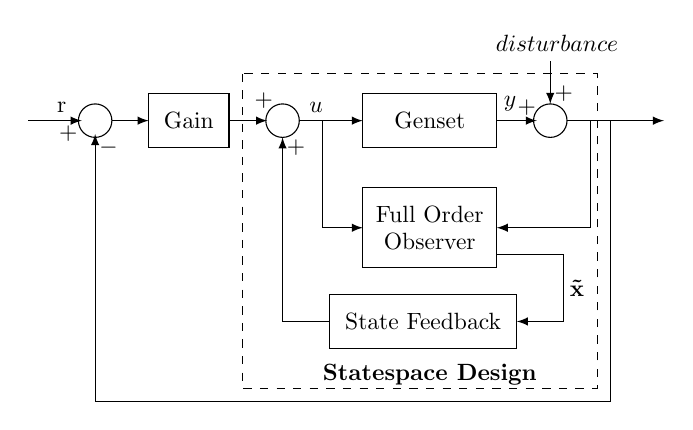
\begin{tikzpicture} [scale=0.85,transform shape]
 \draw [-latex] (-0.2,2) ellipse (0.25 and 0.25);
 \node at (2,2) {\normalsize{Genset}};
\draw [-latex] (1,2.4) rectangle (3,1.6);
 \node at (2,0.2) {\normalsize{Observer}};
  \node at (2,0.6) {\normalsize{Full Order}};
\draw [-latex] (1,1) rectangle (3,-0.2);
\draw [-latex](0.05,2) -- (1,2);
\draw [-latex](0.4,2) -- (0.4,0.4) -- (1,0.4);
\draw [-latex](4.4,2) -- (4.4,0.4) -- (3,0.4);
 \node at (1.9,-1) {\normalsize{State Feedback}};
\draw [-latex] (0.5,-0.6) rectangle (3.3,-1.4);
  \node at (-1.6,2) {\normalsize{Gain}};
\draw [-latex](-1,2) -- (-0.43,2);
\node at (3.2,2.25) {\normalsize{$y$}};
\node at (0.3,2.2) {\normalsize{$u$}};
\node at (4.2,-0.5) {\normalsize{$\mathbf{\tilde{x}}$}};
\draw [-latex] (-2.2,2.4) rectangle (-1,1.6);
\draw [-latex] (-3,2) ellipse (0.25 and 0.25);
 \draw [-latex] (3.8,2) ellipse (0.25 and 0.25);
\draw [-latex](3,2) -- (3.6,2);
\draw [-latex](4.05,2) -- (5.5,2);
\draw [-latex](-2.75,2) -- (-2.2,2);
\draw [-latex](-4,2) -- (-3.2,2);
\draw [-latex](4.7,2) -- (4.7,-2.2) -- (-3,-2.2) -- (-3,1.8);
 \node at (3.9,3.15) {\normalsize{$disturbance$}};
 \node at (4,2.4) {$+$};
\node at (-2.8,1.6) {$-$};
\node at (-3.4,1.8) {$+$};
\node at (-3.5,2.2) {r };
\draw [dashed] (-0.8,2.7) rectangle (4.5,-2);
\node at (2,-1.8) {\textbf{{\normalsize{Statespace Design}}}};
\node at (-0.48,2.3) {$+$};
\node at (0,1.6) {$+$};
\draw [-latex](0.5,-1) -- (-0.2,-1) -- (-0.2,1.75);
\draw [-latex](3,0) -- (4,0) -- (4,-1) -- (3.3,-1);
\draw [-latex](3.8,2.89) -- (3.8,2.25);
\node at (3.45,2.2) {$+$};
\end{tikzpicture}

 
% \end{figure}


\end{frame}


%%%%%%%%%%%%%%%%
\section{Results}
%%%%%%%%%%%% MID WAY AGENDA %%%%%%%%%%%%%%
%\begin{frame}<beamer>
%\frametitle{Thomas Holm Pilgaard}
%\tableofcontents[currentsection]
%\end{frame}
%%%%%%%%%%%% MID WAY AGENDA %%%%%%%%%%%%%%

\begin{frame}{Results}{}
% \begin{figure}[H]
% \centering
% % This file was created by matlab2tikz.
%
%The latest updates can be retrieved from
%  http://www.mathworks.com/matlabcentral/fileexchange/22022-matlab2tikz-matlab2tikz
%where you can also make suggestions and rate matlab2tikz.
%
\definecolor{mycolor1}{rgb}{1.00000,1.00000,0.06667}%
\definecolor{mycolor2}{rgb}{0.07451,0.62353,1.00000}%
\definecolor{mycolor3}{rgb}{0.68627,0.68627,0.68627}%
\definecolor{mycolor4}{rgb}{0.88206,0.88206,0.88206}%
%
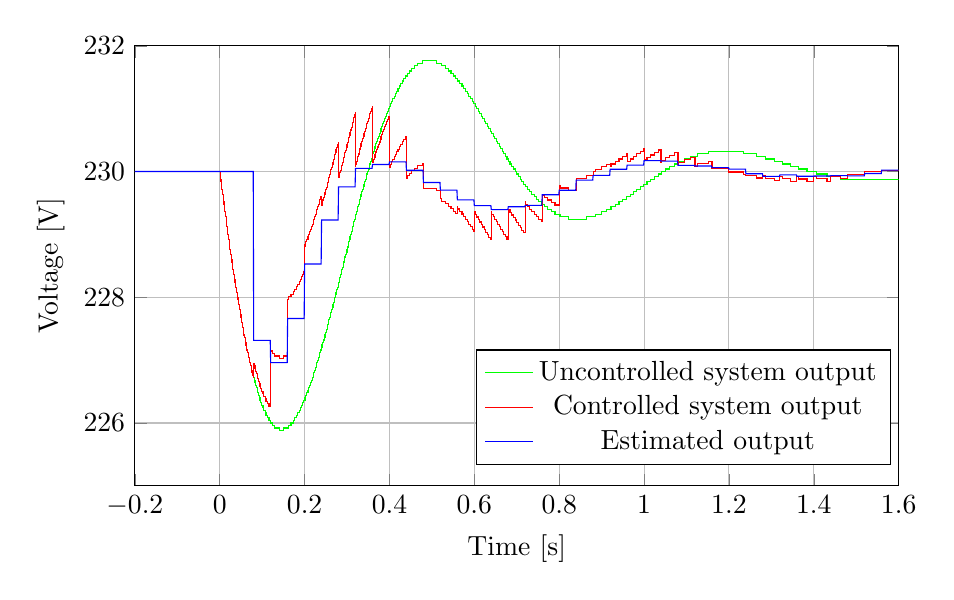
\begin{tikzpicture}

\begin{axis}[%
{width=0.8\columnwidth},
height=2.2in,
at={(0.758in,0.481in)},
scale only axis,
xmin=-0.2,
xmax=1.6,
xlabel={Time [s]},
xmajorgrids,
ymin=225,
ymax=232,
ylabel={Voltage [V]},
ymajorgrids,
axis background/.style={fill=white},
title style={font=\bfseries},
legend style={at={(0.99,0.31)},anchor=north east},
y filter/.code={\pgfmathparse{\pgfmathresult+230.}\pgfmathresult},
x filter/.code={\pgfmathparse{\pgfmathresult-10.}\pgfmathresult}
]
\addplot[const plot,color=green,solid] plot table[row sep=crcr] {%
9.609	0\\
9.61	0\\
9.611	0\\
9.612	0\\
9.613	0\\
9.614	0\\
9.615	0\\
9.616	0\\
9.617	0\\
9.618	0\\
9.619	0\\
9.62	0\\
9.621	0\\
9.622	0\\
9.623	0\\
9.624	0\\
9.625	0\\
9.626	0\\
9.627	0\\
9.628	0\\
9.629	0\\
9.63	0\\
9.631	0\\
9.632	0\\
9.633	0\\
9.634	0\\
9.635	0\\
9.636	0\\
9.637	0\\
9.638	0\\
9.639	0\\
9.64	0\\
9.641	0\\
9.642	0\\
9.643	0\\
9.644	0\\
9.645	0\\
9.646	0\\
9.647	0\\
9.648	0\\
9.649	0\\
9.65	0\\
9.651	0\\
9.652	0\\
9.653	0\\
9.654	0\\
9.655	0\\
9.656	0\\
9.657	0\\
9.658	0\\
9.659	0\\
9.66	0\\
9.661	0\\
9.662	0\\
9.663	0\\
9.664	0\\
9.665	0\\
9.666	0\\
9.667	0\\
9.668	0\\
9.669	0\\
9.67	0\\
9.671	0\\
9.672	0\\
9.673	0\\
9.674	0\\
9.675	0\\
9.676	0\\
9.677	0\\
9.678	0\\
9.679	0\\
9.68	0\\
9.681	0\\
9.682	0\\
9.683	0\\
9.684	0\\
9.685	0\\
9.686	0\\
9.687	0\\
9.688	0\\
9.689	0\\
9.69	0\\
9.691	0\\
9.692	0\\
9.693	0\\
9.694	0\\
9.695	0\\
9.696	0\\
9.697	0\\
9.698	0\\
9.699	0\\
9.7	0\\
9.701	0\\
9.702	0\\
9.703	0\\
9.704	0\\
9.705	0\\
9.706	0\\
9.707	0\\
9.708	0\\
9.709	0\\
9.71	0\\
9.711	0\\
9.712	0\\
9.713	0\\
9.714	0\\
9.715	0\\
9.716	0\\
9.717	0\\
9.718	0\\
9.719	0\\
9.72	0\\
9.721	0\\
9.722	0\\
9.723	0\\
9.724	0\\
9.725	0\\
9.726	0\\
9.727	0\\
9.728	0\\
9.729	0\\
9.73	0\\
9.731	0\\
9.732	0\\
9.733	0\\
9.734	0\\
9.735	0\\
9.736	0\\
9.737	0\\
9.738	0\\
9.739	0\\
9.74	0\\
9.741	0\\
9.742	0\\
9.743	0\\
9.744	0\\
9.745	0\\
9.746	0\\
9.747	0\\
9.748	0\\
9.749	0\\
9.75	0\\
9.751	0\\
9.752	0\\
9.753	0\\
9.754	0\\
9.755	0\\
9.756	0\\
9.757	0\\
9.758	0\\
9.759	-0\\
9.76	-0\\
9.761	-0\\
9.762	-0\\
9.763	-0\\
9.764	-0\\
9.765	-0\\
9.766	-0\\
9.767	-0\\
9.768	-0\\
9.769	-0\\
9.77	-0\\
9.771	-0\\
9.772	-0\\
9.773	-0\\
9.774	-0\\
9.775	-0\\
9.776	-0\\
9.777	-0\\
9.778	-0\\
9.779	-0\\
9.78	-0\\
9.781	-0\\
9.782	-0\\
9.783	-0\\
9.784	-0\\
9.785	-0\\
9.786	-0\\
9.787	-0\\
9.788	-0\\
9.789	-0\\
9.79	-0\\
9.791	-0\\
9.792	-0\\
9.793	-0\\
9.794	-0\\
9.795	-0\\
9.796	-0\\
9.797	-0\\
9.798	-0\\
9.799	-0\\
9.8	-0\\
9.801	-0\\
9.802	-0\\
9.803	-0\\
9.804	-0\\
9.805	-0\\
9.806	-0\\
9.807	-0\\
9.808	-0\\
9.809	-0\\
9.81	-0\\
9.811	-0\\
9.812	-0\\
9.813	-0\\
9.814	-0\\
9.815	-0\\
9.816	-0\\
9.817	-0\\
9.818	-0\\
9.819	-0\\
9.82	-0\\
9.821	-0\\
9.822	-0\\
9.823	-0\\
9.824	-0\\
9.825	-0\\
9.826	-0\\
9.827	-0\\
9.828	-0\\
9.829	-0\\
9.83	-0\\
9.831	-0\\
9.832	-0\\
9.833	-0\\
9.834	-0\\
9.835	-0\\
9.836	-0\\
9.837	-0\\
9.838	-0\\
9.839	-0\\
9.84	-0\\
9.841	-0\\
9.842	-0\\
9.843	-0\\
9.844	-0\\
9.845	-0\\
9.846	-0\\
9.847	-0\\
9.848	-0\\
9.849	-0\\
9.85	-0\\
9.851	-0\\
9.852	-0\\
9.853	-0\\
9.854	-0\\
9.855	-0\\
9.856	-0\\
9.857	-0\\
9.858	-0\\
9.859	-0\\
9.86	-0\\
9.861	-0\\
9.862	-0\\
9.863	-0\\
9.864	-0\\
9.865	-0\\
9.866	-0\\
9.867	-0\\
9.868	-0\\
9.869	-0\\
9.87	-0\\
9.871	-0\\
9.872	-0\\
9.873	-0\\
9.874	-0\\
9.875	-0\\
9.876	-0\\
9.877	-0\\
9.878	-0\\
9.879	-0\\
9.88	-0\\
9.881	-0\\
9.882	-0\\
9.883	-0\\
9.884	-0\\
9.885	-0\\
9.886	-0\\
9.887	-0\\
9.888	-0\\
9.889	-0\\
9.89	-0\\
9.891	-0\\
9.892	-0\\
9.893	-0\\
9.894	-0\\
9.895	-0\\
9.896	-0\\
9.897	-0\\
9.898	-0\\
9.899	-0\\
9.9	-0\\
9.901	-0\\
9.902	-0\\
9.903	-0\\
9.904	-0\\
9.905	-0\\
9.906	-0\\
9.907	-0\\
9.908	-0\\
9.909	-0\\
9.91	-0\\
9.911	-0\\
9.912	-0\\
9.913	-0\\
9.914	-0\\
9.915	-0\\
9.916	-0\\
9.917	-0\\
9.918	-0\\
9.919	-0\\
9.92	-0\\
9.921	-0\\
9.922	-0\\
9.923	-0\\
9.924	-0\\
9.925	-0\\
9.926	-0\\
9.927	-0\\
9.928	-0\\
9.929	-0\\
9.93	-0\\
9.931	-0\\
9.932	-0\\
9.933	-0\\
9.934	-0\\
9.935	-0\\
9.936	-0\\
9.937	-0\\
9.938	-0\\
9.939	-0\\
9.94	-0\\
9.941	-0\\
9.942	-0\\
9.943	-0\\
9.944	-0\\
9.945	-0\\
9.946	-0\\
9.947	-0\\
9.948	-0\\
9.949	-0\\
9.95	-0\\
9.951	-0\\
9.952	-0\\
9.953	-0\\
9.954	-0\\
9.955	-0\\
9.956	-0\\
9.957	-0\\
9.958	-0\\
9.959	-0\\
9.96	-0\\
9.961	-0\\
9.962	-0\\
9.963	-0\\
9.964	-0\\
9.965	-0\\
9.966	-0\\
9.967	-0\\
9.968	-0\\
9.969	-0\\
9.97	-0\\
9.971	-0\\
9.972	-0\\
9.973	-0\\
9.974	-0\\
9.975	-0\\
9.976	-0\\
9.977	-0\\
9.978	-0\\
9.979	-0\\
9.98	-0\\
9.981	-0\\
9.982	-0\\
9.983	-0\\
9.984	-0\\
9.985	-0\\
9.986	-0\\
9.987	-0\\
9.988	-0\\
9.989	-0\\
9.99	-0\\
9.991	-0\\
9.992	-0\\
9.993	-0\\
9.994	-0\\
9.995	-0\\
9.996	-0\\
9.997	-0\\
9.998	-0\\
9.999	-0\\
10	-0\\
10.0000000000001	-0\\
10.0000000000002	-0\\
10.001	-0.04\\
10.002	-0.12\\
10.003	-0.16\\
10.004	-0.2\\
10.005	-0.28\\
10.006	-0.32\\
10.007	-0.36\\
10.008	-0.44\\
10.009	-0.48\\
10.01	-0.52\\
10.011	-0.6\\
10.012	-0.64\\
10.013	-0.68\\
10.014	-0.72\\
10.015	-0.8\\
10.016	-0.84\\
10.017	-0.88\\
10.018	-0.92\\
10.019	-1\\
10.02	-1.04\\
10.021	-1.08\\
10.022	-1.12\\
10.023	-1.16\\
10.024	-1.24\\
10.025	-1.28\\
10.026	-1.32\\
10.027	-1.36\\
10.028	-1.4\\
10.029	-1.44\\
10.03	-1.52\\
10.031	-1.56\\
10.032	-1.6\\
10.033	-1.64\\
10.034	-1.68\\
10.035	-1.72\\
10.036	-1.76\\
10.037	-1.8\\
10.038	-1.84\\
10.039	-1.88\\
10.04	-1.92\\
10.041	-1.96\\
10.042	-2\\
10.043	-2.04\\
10.044	-2.08\\
10.045	-2.12\\
10.046	-2.16\\
10.047	-2.2\\
10.048	-2.24\\
10.049	-2.28\\
10.05	-2.32\\
10.051	-2.36\\
10.052	-2.4\\
10.053	-2.44\\
10.054	-2.48\\
10.055	-2.52\\
10.056	-2.56\\
10.057	-2.6\\
10.058	-2.64\\
10.059	-2.64\\
10.06	-2.68\\
10.061	-2.72\\
10.062	-2.76\\
10.063	-2.8\\
10.064	-2.84\\
10.065	-2.84\\
10.066	-2.88\\
10.067	-2.92\\
10.068	-2.96\\
10.069	-2.96\\
10.07	-3\\
10.071	-3.04\\
10.072	-3.08\\
10.073	-3.08\\
10.074	-3.12\\
10.075	-3.16\\
10.076	-3.2\\
10.077	-3.2\\
10.078	-3.24\\
10.079	-3.28\\
10.08	-3.28\\
10.081	-3.32\\
10.082	-3.32\\
10.083	-3.36\\
10.084	-3.4\\
10.085	-3.4\\
10.086	-3.44\\
10.087	-3.44\\
10.088	-3.48\\
10.089	-3.52\\
10.09	-3.52\\
10.091	-3.56\\
10.092	-3.56\\
10.093	-3.6\\
10.094	-3.6\\
10.095	-3.64\\
10.096	-3.64\\
10.097	-3.68\\
10.098	-3.68\\
10.099	-3.72\\
10.1	-3.72\\
10.101	-3.72\\
10.102	-3.76\\
10.103	-3.76\\
10.104	-3.8\\
10.105	-3.8\\
10.106	-3.8\\
10.107	-3.84\\
10.108	-3.84\\
10.109	-3.88\\
10.11	-3.88\\
10.111	-3.88\\
10.112	-3.92\\
10.113	-3.92\\
10.114	-3.92\\
10.115	-3.92\\
10.116	-3.96\\
10.117	-3.96\\
10.118	-3.96\\
10.119	-3.96\\
10.12	-4\\
10.121	-4\\
10.122	-4\\
10.123	-4\\
10.124	-4.04\\
10.125	-4.04\\
10.126	-4.04\\
10.127	-4.04\\
10.128	-4.04\\
10.129	-4.04\\
10.13	-4.08\\
10.131	-4.08\\
10.132	-4.08\\
10.133	-4.08\\
10.134	-4.08\\
10.135	-4.08\\
10.136	-4.08\\
10.137	-4.08\\
10.138	-4.08\\
10.139	-4.08\\
10.14	-4.12\\
10.141	-4.12\\
10.142	-4.12\\
10.143	-4.12\\
10.144	-4.12\\
10.145	-4.12\\
10.146	-4.12\\
10.147	-4.12\\
10.148	-4.12\\
10.149	-4.12\\
10.15	-4.12\\
10.151	-4.08\\
10.152	-4.08\\
10.153	-4.08\\
10.154	-4.08\\
10.155	-4.08\\
10.156	-4.08\\
10.157	-4.08\\
10.158	-4.08\\
10.159	-4.08\\
10.16	-4.08\\
10.161	-4.08\\
10.162	-4.04\\
10.163	-4.04\\
10.164	-4.04\\
10.165	-4.04\\
10.166	-4.04\\
10.167	-4.04\\
10.168	-4\\
10.169	-4\\
10.17	-4\\
10.171	-4\\
10.172	-4\\
10.173	-3.96\\
10.174	-3.96\\
10.175	-3.96\\
10.176	-3.96\\
10.177	-3.92\\
10.178	-3.92\\
10.179	-3.92\\
10.18	-3.92\\
10.181	-3.88\\
10.182	-3.88\\
10.183	-3.88\\
10.184	-3.84\\
10.185	-3.84\\
10.186	-3.84\\
10.187	-3.8\\
10.188	-3.8\\
10.189	-3.8\\
10.19	-3.76\\
10.191	-3.76\\
10.192	-3.76\\
10.193	-3.72\\
10.194	-3.72\\
10.195	-3.72\\
10.196	-3.68\\
10.197	-3.68\\
10.198	-3.64\\
10.199	-3.64\\
10.2	-3.64\\
10.201	-3.6\\
10.202	-3.6\\
10.203	-3.56\\
10.204	-3.56\\
10.205	-3.52\\
10.206	-3.52\\
10.207	-3.52\\
10.208	-3.48\\
10.209	-3.48\\
10.21	-3.44\\
10.211	-3.44\\
10.212	-3.4\\
10.213	-3.4\\
10.214	-3.36\\
10.215	-3.36\\
10.216	-3.32\\
10.217	-3.32\\
10.218	-3.28\\
10.219	-3.28\\
10.22	-3.24\\
10.221	-3.24\\
10.222	-3.2\\
10.223	-3.2\\
10.224	-3.16\\
10.225	-3.16\\
10.226	-3.12\\
10.227	-3.08\\
10.228	-3.08\\
10.229	-3.04\\
10.23	-3.04\\
10.231	-3\\
10.232	-3\\
10.233	-2.96\\
10.234	-2.96\\
10.235	-2.92\\
10.236	-2.88\\
10.237	-2.88\\
10.238	-2.84\\
10.239	-2.84\\
10.24	-2.8\\
10.241	-2.76\\
10.242	-2.76\\
10.243	-2.72\\
10.244	-2.72\\
10.245	-2.68\\
10.246	-2.64\\
10.247	-2.64\\
10.248	-2.6\\
10.249	-2.6\\
10.25	-2.56\\
10.251	-2.52\\
10.252	-2.52\\
10.253	-2.48\\
10.254	-2.44\\
10.255	-2.44\\
10.256	-2.4\\
10.257	-2.36\\
10.258	-2.36\\
10.259	-2.32\\
10.26	-2.32\\
10.261	-2.28\\
10.262	-2.24\\
10.263	-2.24\\
10.264	-2.2\\
10.265	-2.16\\
10.266	-2.16\\
10.267	-2.12\\
10.268	-2.08\\
10.269	-2.08\\
10.27	-2.04\\
10.271	-2\\
10.272	-2\\
10.273	-1.96\\
10.274	-1.92\\
10.275	-1.92\\
10.276	-1.88\\
10.277	-1.84\\
10.278	-1.84\\
10.279	-1.8\\
10.28	-1.76\\
10.281	-1.76\\
10.282	-1.72\\
10.283	-1.68\\
10.284	-1.68\\
10.285	-1.64\\
10.286	-1.6\\
10.287	-1.6\\
10.288	-1.56\\
10.289	-1.52\\
10.29	-1.52\\
10.291	-1.48\\
10.292	-1.44\\
10.293	-1.44\\
10.294	-1.4\\
10.295	-1.36\\
10.296	-1.36\\
10.297	-1.32\\
10.298	-1.28\\
10.299	-1.28\\
10.3	-1.24\\
10.301	-1.2\\
10.302	-1.2\\
10.303	-1.16\\
10.304	-1.12\\
10.305	-1.12\\
10.306	-1.08\\
10.307	-1.04\\
10.308	-1.04\\
10.309	-1\\
10.31	-0.96\\
10.311	-0.96\\
10.312	-0.92\\
10.313	-0.88\\
10.314	-0.88\\
10.315	-0.84\\
10.316	-0.8\\
10.317	-0.8\\
10.318	-0.76\\
10.319	-0.72\\
10.32	-0.72\\
10.321	-0.68\\
10.322	-0.64\\
10.323	-0.64\\
10.324	-0.6\\
10.325	-0.56\\
10.326	-0.56\\
10.327	-0.52\\
10.328	-0.52\\
10.329	-0.48\\
10.33	-0.44\\
10.331	-0.44\\
10.332	-0.4\\
10.333	-0.36\\
10.334	-0.36\\
10.335	-0.32\\
10.336	-0.32\\
10.337	-0.28\\
10.338	-0.24\\
10.339	-0.24\\
10.34	-0.2\\
10.341	-0.16\\
10.342	-0.16\\
10.343	-0.12\\
10.344	-0.12\\
10.345	-0.08\\
10.346	-0.04\\
10.347	-0.04\\
10.348	-0\\
10.349	0\\
10.35	0.04\\
10.351	0.04\\
10.352	0.08\\
10.353	0.12\\
10.354	0.12\\
10.355	0.16\\
10.356	0.16\\
10.357	0.2\\
10.358	0.2\\
10.359	0.24\\
10.36	0.28\\
10.361	0.28\\
10.362	0.32\\
10.363	0.32\\
10.364	0.36\\
10.365	0.36\\
10.366	0.4\\
10.367	0.4\\
10.368	0.44\\
10.369	0.44\\
10.37	0.48\\
10.371	0.48\\
10.372	0.52\\
10.373	0.52\\
10.374	0.56\\
10.375	0.56\\
10.376	0.6\\
10.377	0.6\\
10.378	0.64\\
10.379	0.64\\
10.38	0.68\\
10.381	0.68\\
10.382	0.72\\
10.383	0.72\\
10.384	0.76\\
10.385	0.76\\
10.386	0.8\\
10.387	0.8\\
10.388	0.84\\
10.389	0.84\\
10.39	0.84\\
10.391	0.88\\
10.392	0.88\\
10.393	0.92\\
10.394	0.92\\
10.395	0.96\\
10.396	0.96\\
10.397	0.96\\
10.398	1\\
10.399	1\\
10.4	1.04\\
10.401	1.04\\
10.402	1.04\\
10.403	1.08\\
10.404	1.08\\
10.405	1.12\\
10.406	1.12\\
10.407	1.12\\
10.408	1.16\\
10.409	1.16\\
10.41	1.16\\
10.411	1.2\\
10.412	1.2\\
10.413	1.2\\
10.414	1.24\\
10.415	1.24\\
10.416	1.24\\
10.417	1.28\\
10.418	1.28\\
10.419	1.28\\
10.42	1.32\\
10.421	1.32\\
10.422	1.32\\
10.423	1.36\\
10.424	1.36\\
10.425	1.36\\
10.426	1.4\\
10.427	1.4\\
10.428	1.4\\
10.429	1.4\\
10.43	1.44\\
10.431	1.44\\
10.432	1.44\\
10.433	1.44\\
10.434	1.48\\
10.435	1.48\\
10.436	1.48\\
10.437	1.48\\
10.438	1.52\\
10.439	1.52\\
10.44	1.52\\
10.441	1.52\\
10.442	1.56\\
10.443	1.56\\
10.444	1.56\\
10.445	1.56\\
10.446	1.56\\
10.447	1.6\\
10.448	1.6\\
10.449	1.6\\
10.45	1.6\\
10.451	1.6\\
10.452	1.64\\
10.453	1.64\\
10.454	1.64\\
10.455	1.64\\
10.456	1.64\\
10.457	1.64\\
10.458	1.64\\
10.459	1.68\\
10.46	1.68\\
10.461	1.68\\
10.462	1.68\\
10.463	1.68\\
10.464	1.68\\
10.465	1.68\\
10.466	1.72\\
10.467	1.72\\
10.468	1.72\\
10.469	1.72\\
10.47	1.72\\
10.471	1.72\\
10.472	1.72\\
10.473	1.72\\
10.474	1.72\\
10.475	1.72\\
10.476	1.72\\
10.477	1.76\\
10.478	1.76\\
10.479	1.76\\
10.48	1.76\\
10.481	1.76\\
10.482	1.76\\
10.483	1.76\\
10.484	1.76\\
10.485	1.76\\
10.486	1.76\\
10.487	1.76\\
10.488	1.76\\
10.489	1.76\\
10.49	1.76\\
10.491	1.76\\
10.492	1.76\\
10.493	1.76\\
10.494	1.76\\
10.495	1.76\\
10.496	1.76\\
10.497	1.76\\
10.498	1.76\\
10.499	1.76\\
10.5	1.76\\
10.501	1.76\\
10.502	1.76\\
10.503	1.76\\
10.504	1.76\\
10.505	1.76\\
10.506	1.76\\
10.507	1.76\\
10.508	1.76\\
10.509	1.76\\
10.51	1.76\\
10.511	1.72\\
10.512	1.72\\
10.513	1.72\\
10.514	1.72\\
10.515	1.72\\
10.516	1.72\\
10.517	1.72\\
10.518	1.72\\
10.519	1.72\\
10.52	1.72\\
10.521	1.72\\
10.522	1.72\\
10.523	1.68\\
10.524	1.68\\
10.525	1.68\\
10.526	1.68\\
10.527	1.68\\
10.528	1.68\\
10.529	1.68\\
10.53	1.68\\
10.531	1.68\\
10.532	1.64\\
10.533	1.64\\
10.534	1.64\\
10.535	1.64\\
10.536	1.64\\
10.537	1.64\\
10.538	1.64\\
10.539	1.6\\
10.54	1.6\\
10.541	1.6\\
10.542	1.6\\
10.543	1.6\\
10.544	1.6\\
10.545	1.56\\
10.546	1.56\\
10.547	1.56\\
10.548	1.56\\
10.549	1.56\\
10.55	1.56\\
10.551	1.52\\
10.552	1.52\\
10.553	1.52\\
10.554	1.52\\
10.555	1.52\\
10.556	1.48\\
10.557	1.48\\
10.558	1.48\\
10.559	1.48\\
10.56	1.48\\
10.561	1.44\\
10.562	1.44\\
10.563	1.44\\
10.564	1.44\\
10.565	1.44\\
10.566	1.4\\
10.567	1.4\\
10.568	1.4\\
10.569	1.4\\
10.57	1.4\\
10.571	1.36\\
10.572	1.36\\
10.573	1.36\\
10.574	1.36\\
10.575	1.32\\
10.576	1.32\\
10.577	1.32\\
10.578	1.32\\
10.579	1.28\\
10.58	1.28\\
10.581	1.28\\
10.582	1.28\\
10.583	1.24\\
10.584	1.24\\
10.585	1.24\\
10.586	1.24\\
10.587	1.2\\
10.588	1.2\\
10.589	1.2\\
10.59	1.2\\
10.591	1.16\\
10.592	1.16\\
10.593	1.16\\
10.594	1.16\\
10.595	1.12\\
10.596	1.12\\
10.597	1.12\\
10.598	1.12\\
10.599	1.08\\
10.6	1.08\\
10.601	1.08\\
10.602	1.04\\
10.603	1.04\\
10.604	1.04\\
10.605	1.04\\
10.606	1\\
10.607	1\\
10.608	1\\
10.609	1\\
10.61	0.96\\
10.611	0.96\\
10.612	0.96\\
10.613	0.92\\
10.614	0.92\\
10.615	0.92\\
10.616	0.92\\
10.617	0.88\\
10.618	0.88\\
10.619	0.88\\
10.62	0.84\\
10.621	0.84\\
10.622	0.84\\
10.623	0.84\\
10.624	0.8\\
10.625	0.8\\
10.626	0.8\\
10.627	0.76\\
10.628	0.76\\
10.629	0.76\\
10.63	0.76\\
10.631	0.72\\
10.632	0.72\\
10.633	0.72\\
10.634	0.68\\
10.635	0.68\\
10.636	0.68\\
10.637	0.68\\
10.638	0.64\\
10.639	0.64\\
10.64	0.64\\
10.641	0.6\\
10.642	0.6\\
10.643	0.6\\
10.644	0.6\\
10.645	0.56\\
10.646	0.56\\
10.647	0.56\\
10.648	0.52\\
10.649	0.52\\
10.65	0.52\\
10.651	0.52\\
10.652	0.48\\
10.653	0.48\\
10.654	0.48\\
10.655	0.44\\
10.656	0.44\\
10.657	0.44\\
10.658	0.44\\
10.659	0.4\\
10.66	0.4\\
10.661	0.4\\
10.662	0.36\\
10.663	0.36\\
10.664	0.36\\
10.665	0.36\\
10.666	0.32\\
10.667	0.32\\
10.668	0.32\\
10.669	0.28\\
10.67	0.28\\
10.671	0.28\\
10.672	0.28\\
10.673	0.24\\
10.674	0.24\\
10.675	0.24\\
10.676	0.24\\
10.677	0.2\\
10.678	0.2\\
10.679	0.2\\
10.68	0.16\\
10.681	0.16\\
10.682	0.16\\
10.683	0.16\\
10.684	0.12\\
10.685	0.12\\
10.686	0.12\\
10.687	0.12\\
10.688	0.08\\
10.689	0.08\\
10.69	0.08\\
10.691	0.08\\
10.692	0.04\\
10.693	0.04\\
10.694	0.04\\
10.695	0.04\\
10.696	0\\
10.697	0\\
10.698	-0\\
10.699	-0\\
10.7	-0.04\\
10.701	-0.04\\
10.702	-0.04\\
10.703	-0.04\\
10.704	-0.08\\
10.705	-0.08\\
10.706	-0.08\\
10.707	-0.08\\
10.708	-0.12\\
10.709	-0.12\\
10.71	-0.12\\
10.711	-0.12\\
10.712	-0.16\\
10.713	-0.16\\
10.714	-0.16\\
10.715	-0.16\\
10.716	-0.2\\
10.717	-0.2\\
10.718	-0.2\\
10.719	-0.2\\
10.72	-0.2\\
10.721	-0.24\\
10.722	-0.24\\
10.723	-0.24\\
10.724	-0.24\\
10.725	-0.24\\
10.726	-0.28\\
10.727	-0.28\\
10.728	-0.28\\
10.729	-0.28\\
10.73	-0.32\\
10.731	-0.32\\
10.732	-0.32\\
10.733	-0.32\\
10.734	-0.32\\
10.735	-0.36\\
10.736	-0.36\\
10.737	-0.36\\
10.738	-0.36\\
10.739	-0.36\\
10.74	-0.36\\
10.741	-0.4\\
10.742	-0.4\\
10.743	-0.4\\
10.744	-0.4\\
10.745	-0.4\\
10.746	-0.44\\
10.747	-0.44\\
10.748	-0.44\\
10.749	-0.44\\
10.75	-0.44\\
10.751	-0.44\\
10.752	-0.48\\
10.753	-0.48\\
10.754	-0.48\\
10.755	-0.48\\
10.756	-0.48\\
10.757	-0.48\\
10.758	-0.52\\
10.759	-0.52\\
10.76	-0.52\\
10.761	-0.52\\
10.762	-0.52\\
10.763	-0.52\\
10.764	-0.52\\
10.765	-0.56\\
10.766	-0.56\\
10.767	-0.56\\
10.768	-0.56\\
10.769	-0.56\\
10.77	-0.56\\
10.771	-0.56\\
10.772	-0.6\\
10.773	-0.6\\
10.774	-0.6\\
10.775	-0.6\\
10.776	-0.6\\
10.777	-0.6\\
10.778	-0.6\\
10.779	-0.6\\
10.78	-0.6\\
10.781	-0.64\\
10.782	-0.64\\
10.783	-0.64\\
10.784	-0.64\\
10.785	-0.64\\
10.786	-0.64\\
10.787	-0.64\\
10.788	-0.64\\
10.789	-0.64\\
10.79	-0.68\\
10.791	-0.68\\
10.792	-0.68\\
10.793	-0.68\\
10.794	-0.68\\
10.795	-0.68\\
10.796	-0.68\\
10.797	-0.68\\
10.798	-0.68\\
10.799	-0.68\\
10.8	-0.68\\
10.801	-0.68\\
10.802	-0.72\\
10.803	-0.72\\
10.804	-0.72\\
10.805	-0.72\\
10.806	-0.72\\
10.807	-0.72\\
10.808	-0.72\\
10.809	-0.72\\
10.81	-0.72\\
10.811	-0.72\\
10.812	-0.72\\
10.813	-0.72\\
10.814	-0.72\\
10.815	-0.72\\
10.816	-0.72\\
10.817	-0.72\\
10.818	-0.72\\
10.819	-0.72\\
10.82	-0.72\\
10.821	-0.76\\
10.822	-0.76\\
10.823	-0.76\\
10.824	-0.76\\
10.825	-0.76\\
10.826	-0.76\\
10.827	-0.76\\
10.828	-0.76\\
10.829	-0.76\\
10.83	-0.76\\
10.831	-0.76\\
10.832	-0.76\\
10.833	-0.76\\
10.834	-0.76\\
10.835	-0.76\\
10.836	-0.76\\
10.837	-0.76\\
10.838	-0.76\\
10.839	-0.76\\
10.84	-0.76\\
10.841	-0.76\\
10.842	-0.76\\
10.843	-0.76\\
10.844	-0.76\\
10.845	-0.76\\
10.846	-0.76\\
10.847	-0.76\\
10.848	-0.76\\
10.849	-0.76\\
10.85	-0.76\\
10.851	-0.76\\
10.852	-0.76\\
10.853	-0.76\\
10.854	-0.76\\
10.855	-0.76\\
10.856	-0.76\\
10.857	-0.76\\
10.858	-0.76\\
10.859	-0.76\\
10.86	-0.76\\
10.861	-0.76\\
10.862	-0.76\\
10.863	-0.76\\
10.864	-0.76\\
10.865	-0.72\\
10.866	-0.72\\
10.867	-0.72\\
10.868	-0.72\\
10.869	-0.72\\
10.87	-0.72\\
10.871	-0.72\\
10.872	-0.72\\
10.873	-0.72\\
10.874	-0.72\\
10.875	-0.72\\
10.876	-0.72\\
10.877	-0.72\\
10.878	-0.72\\
10.879	-0.72\\
10.88	-0.72\\
10.881	-0.72\\
10.882	-0.72\\
10.883	-0.72\\
10.884	-0.72\\
10.885	-0.72\\
10.886	-0.68\\
10.887	-0.68\\
10.888	-0.68\\
10.889	-0.68\\
10.89	-0.68\\
10.891	-0.68\\
10.892	-0.68\\
10.893	-0.68\\
10.894	-0.68\\
10.895	-0.68\\
10.896	-0.68\\
10.897	-0.68\\
10.898	-0.68\\
10.899	-0.68\\
10.9	-0.64\\
10.901	-0.64\\
10.902	-0.64\\
10.903	-0.64\\
10.904	-0.64\\
10.905	-0.64\\
10.906	-0.64\\
10.907	-0.64\\
10.908	-0.64\\
10.909	-0.64\\
10.91	-0.64\\
10.911	-0.64\\
10.912	-0.6\\
10.913	-0.6\\
10.914	-0.6\\
10.915	-0.6\\
10.916	-0.6\\
10.917	-0.6\\
10.918	-0.6\\
10.919	-0.6\\
10.92	-0.6\\
10.921	-0.6\\
10.922	-0.56\\
10.923	-0.56\\
10.924	-0.56\\
10.925	-0.56\\
10.926	-0.56\\
10.927	-0.56\\
10.928	-0.56\\
10.929	-0.56\\
10.93	-0.56\\
10.931	-0.56\\
10.932	-0.52\\
10.933	-0.52\\
10.934	-0.52\\
10.935	-0.52\\
10.936	-0.52\\
10.937	-0.52\\
10.938	-0.52\\
10.939	-0.52\\
10.94	-0.52\\
10.941	-0.48\\
10.942	-0.48\\
10.943	-0.48\\
10.944	-0.48\\
10.945	-0.48\\
10.946	-0.48\\
10.947	-0.48\\
10.948	-0.48\\
10.949	-0.48\\
10.95	-0.44\\
10.951	-0.44\\
10.952	-0.44\\
10.953	-0.44\\
10.954	-0.44\\
10.955	-0.44\\
10.956	-0.44\\
10.957	-0.44\\
10.958	-0.4\\
10.959	-0.4\\
10.96	-0.4\\
10.961	-0.4\\
10.962	-0.4\\
10.963	-0.4\\
10.964	-0.4\\
10.965	-0.4\\
10.966	-0.4\\
10.967	-0.36\\
10.968	-0.36\\
10.969	-0.36\\
10.97	-0.36\\
10.971	-0.36\\
10.972	-0.36\\
10.973	-0.36\\
10.974	-0.36\\
10.975	-0.32\\
10.976	-0.32\\
10.977	-0.32\\
10.978	-0.32\\
10.979	-0.32\\
10.98	-0.32\\
10.981	-0.32\\
10.982	-0.32\\
10.983	-0.28\\
10.984	-0.28\\
10.985	-0.28\\
10.986	-0.28\\
10.987	-0.28\\
10.988	-0.28\\
10.989	-0.28\\
10.99	-0.28\\
10.991	-0.24\\
10.992	-0.24\\
10.993	-0.24\\
10.994	-0.24\\
10.995	-0.24\\
10.996	-0.24\\
10.997	-0.24\\
10.998	-0.24\\
10.999	-0.2\\
11	-0.2\\
11.001	-0.2\\
11.002	-0.2\\
11.003	-0.2\\
11.004	-0.2\\
11.005	-0.2\\
11.006	-0.2\\
11.007	-0.16\\
11.008	-0.16\\
11.009	-0.16\\
11.01	-0.16\\
11.011	-0.16\\
11.012	-0.16\\
11.013	-0.16\\
11.014	-0.16\\
11.015	-0.12\\
11.016	-0.12\\
11.017	-0.12\\
11.018	-0.12\\
11.019	-0.12\\
11.02	-0.12\\
11.021	-0.12\\
11.022	-0.12\\
11.023	-0.12\\
11.024	-0.08\\
11.025	-0.08\\
11.026	-0.08\\
11.027	-0.08\\
11.028	-0.08\\
11.029	-0.08\\
11.03	-0.08\\
11.031	-0.08\\
11.032	-0.08\\
11.033	-0.04\\
11.034	-0.04\\
11.035	-0.04\\
11.036	-0.04\\
11.037	-0.04\\
11.038	-0.04\\
11.039	-0.04\\
11.04	-0.04\\
11.041	-0\\
11.042	-0\\
11.043	-0\\
11.044	-0\\
11.045	-0\\
11.046	0\\
11.047	0\\
11.048	0\\
11.049	0\\
11.05	0\\
11.051	0.04\\
11.052	0.04\\
11.053	0.04\\
11.054	0.04\\
11.055	0.04\\
11.056	0.04\\
11.057	0.04\\
11.058	0.04\\
11.059	0.04\\
11.06	0.08\\
11.061	0.08\\
11.062	0.08\\
11.063	0.08\\
11.064	0.08\\
11.065	0.08\\
11.066	0.08\\
11.067	0.08\\
11.068	0.08\\
11.069	0.08\\
11.07	0.08\\
11.071	0.12\\
11.072	0.12\\
11.073	0.12\\
11.074	0.12\\
11.075	0.12\\
11.076	0.12\\
11.077	0.12\\
11.078	0.12\\
11.079	0.12\\
11.08	0.12\\
11.081	0.12\\
11.082	0.16\\
11.083	0.16\\
11.084	0.16\\
11.085	0.16\\
11.086	0.16\\
11.087	0.16\\
11.088	0.16\\
11.089	0.16\\
11.09	0.16\\
11.091	0.16\\
11.092	0.16\\
11.093	0.16\\
11.094	0.16\\
11.095	0.2\\
11.096	0.2\\
11.097	0.2\\
11.098	0.2\\
11.099	0.2\\
11.1	0.2\\
11.101	0.2\\
11.102	0.2\\
11.103	0.2\\
11.104	0.2\\
11.105	0.2\\
11.106	0.2\\
11.107	0.2\\
11.108	0.2\\
11.109	0.24\\
11.11	0.24\\
11.111	0.24\\
11.112	0.24\\
11.113	0.24\\
11.114	0.24\\
11.115	0.24\\
11.116	0.24\\
11.117	0.24\\
11.118	0.24\\
11.119	0.24\\
11.12	0.24\\
11.121	0.24\\
11.122	0.24\\
11.123	0.24\\
11.124	0.24\\
11.125	0.24\\
11.126	0.28\\
11.127	0.28\\
11.128	0.28\\
11.129	0.28\\
11.13	0.28\\
11.131	0.28\\
11.132	0.28\\
11.133	0.28\\
11.134	0.28\\
11.135	0.28\\
11.136	0.28\\
11.137	0.28\\
11.138	0.28\\
11.139	0.28\\
11.14	0.28\\
11.141	0.28\\
11.142	0.28\\
11.143	0.28\\
11.144	0.28\\
11.145	0.28\\
11.146	0.28\\
11.147	0.28\\
11.148	0.28\\
11.149	0.28\\
11.15	0.28\\
11.151	0.32\\
11.152	0.32\\
11.153	0.32\\
11.154	0.32\\
11.155	0.32\\
11.156	0.32\\
11.157	0.32\\
11.158	0.32\\
11.159	0.32\\
11.16	0.32\\
11.161	0.32\\
11.162	0.32\\
11.163	0.32\\
11.164	0.32\\
11.165	0.32\\
11.166	0.32\\
11.167	0.32\\
11.168	0.32\\
11.169	0.32\\
11.17	0.32\\
11.171	0.32\\
11.172	0.32\\
11.173	0.32\\
11.174	0.32\\
11.175	0.32\\
11.176	0.32\\
11.177	0.32\\
11.178	0.32\\
11.179	0.32\\
11.18	0.32\\
11.181	0.32\\
11.182	0.32\\
11.183	0.32\\
11.184	0.32\\
11.185	0.32\\
11.186	0.32\\
11.187	0.32\\
11.188	0.32\\
11.189	0.32\\
11.19	0.32\\
11.191	0.32\\
11.192	0.32\\
11.193	0.32\\
11.194	0.32\\
11.195	0.32\\
11.196	0.32\\
11.197	0.32\\
11.198	0.32\\
11.199	0.32\\
11.2	0.32\\
11.201	0.32\\
11.202	0.32\\
11.203	0.32\\
11.204	0.32\\
11.205	0.32\\
11.206	0.32\\
11.207	0.32\\
11.208	0.32\\
11.209	0.32\\
11.21	0.32\\
11.211	0.32\\
11.212	0.32\\
11.213	0.32\\
11.214	0.32\\
11.215	0.32\\
11.216	0.32\\
11.217	0.32\\
11.218	0.32\\
11.219	0.32\\
11.22	0.32\\
11.221	0.32\\
11.222	0.32\\
11.223	0.32\\
11.224	0.32\\
11.225	0.32\\
11.226	0.32\\
11.227	0.32\\
11.228	0.32\\
11.229	0.32\\
11.23	0.32\\
11.231	0.32\\
11.232	0.32\\
11.233	0.32\\
11.234	0.32\\
11.235	0.28\\
11.236	0.28\\
11.237	0.28\\
11.238	0.28\\
11.239	0.28\\
11.24	0.28\\
11.241	0.28\\
11.242	0.28\\
11.243	0.28\\
11.244	0.28\\
11.245	0.28\\
11.246	0.28\\
11.247	0.28\\
11.248	0.28\\
11.249	0.28\\
11.25	0.28\\
11.251	0.28\\
11.252	0.28\\
11.253	0.28\\
11.254	0.28\\
11.255	0.28\\
11.256	0.28\\
11.257	0.28\\
11.258	0.28\\
11.259	0.28\\
11.26	0.28\\
11.261	0.28\\
11.262	0.28\\
11.263	0.28\\
11.264	0.24\\
11.265	0.24\\
11.266	0.24\\
11.267	0.24\\
11.268	0.24\\
11.269	0.24\\
11.27	0.24\\
11.271	0.24\\
11.272	0.24\\
11.273	0.24\\
11.274	0.24\\
11.275	0.24\\
11.276	0.24\\
11.277	0.24\\
11.278	0.24\\
11.279	0.24\\
11.28	0.24\\
11.281	0.24\\
11.282	0.24\\
11.283	0.24\\
11.284	0.24\\
11.285	0.24\\
11.286	0.24\\
11.287	0.2\\
11.288	0.2\\
11.289	0.2\\
11.29	0.2\\
11.291	0.2\\
11.292	0.2\\
11.293	0.2\\
11.294	0.2\\
11.295	0.2\\
11.296	0.2\\
11.297	0.2\\
11.298	0.2\\
11.299	0.2\\
11.3	0.2\\
11.301	0.2\\
11.302	0.2\\
11.303	0.2\\
11.304	0.2\\
11.305	0.2\\
11.306	0.2\\
11.307	0.16\\
11.308	0.16\\
11.309	0.16\\
11.31	0.16\\
11.311	0.16\\
11.312	0.16\\
11.313	0.16\\
11.314	0.16\\
11.315	0.16\\
11.316	0.16\\
11.317	0.16\\
11.318	0.16\\
11.319	0.16\\
11.32	0.16\\
11.321	0.16\\
11.322	0.16\\
11.323	0.16\\
11.324	0.16\\
11.325	0.16\\
11.326	0.12\\
11.327	0.12\\
11.328	0.12\\
11.329	0.12\\
11.33	0.12\\
11.331	0.12\\
11.332	0.12\\
11.333	0.12\\
11.334	0.12\\
11.335	0.12\\
11.336	0.12\\
11.337	0.12\\
11.338	0.12\\
11.339	0.12\\
11.34	0.12\\
11.341	0.12\\
11.342	0.12\\
11.343	0.12\\
11.344	0.12\\
11.345	0.08\\
11.346	0.08\\
11.347	0.08\\
11.348	0.08\\
11.349	0.08\\
11.35	0.08\\
11.351	0.08\\
11.352	0.08\\
11.353	0.08\\
11.354	0.08\\
11.355	0.08\\
11.356	0.08\\
11.357	0.08\\
11.358	0.08\\
11.359	0.08\\
11.36	0.08\\
11.361	0.08\\
11.362	0.08\\
11.363	0.08\\
11.364	0.04\\
11.365	0.04\\
11.366	0.04\\
11.367	0.04\\
11.368	0.04\\
11.369	0.04\\
11.37	0.04\\
11.371	0.04\\
11.372	0.04\\
11.373	0.04\\
11.374	0.04\\
11.375	0.04\\
11.376	0.04\\
11.377	0.04\\
11.378	0.04\\
11.379	0.04\\
11.38	0.04\\
11.381	0.04\\
11.382	0.04\\
11.383	0.04\\
11.384	0\\
11.385	0\\
11.386	0\\
11.387	0\\
11.388	0\\
11.389	0\\
11.39	0\\
11.391	0\\
11.392	0\\
11.393	0\\
11.394	0\\
11.395	-0\\
11.396	-0\\
11.397	-0\\
11.398	-0\\
11.399	-0\\
11.4	-0\\
11.401	-0\\
11.402	-0\\
11.403	-0\\
11.404	-0\\
11.405	-0\\
11.406	-0.04\\
11.407	-0.04\\
11.408	-0.04\\
11.409	-0.04\\
11.41	-0.04\\
11.411	-0.04\\
11.412	-0.04\\
11.413	-0.04\\
11.414	-0.04\\
11.415	-0.04\\
11.416	-0.04\\
11.417	-0.04\\
11.418	-0.04\\
11.419	-0.04\\
11.42	-0.04\\
11.421	-0.04\\
11.422	-0.04\\
11.423	-0.04\\
11.424	-0.04\\
11.425	-0.04\\
11.426	-0.04\\
11.427	-0.04\\
11.428	-0.04\\
11.429	-0.04\\
11.43	-0.04\\
11.431	-0.08\\
11.432	-0.08\\
11.433	-0.08\\
11.434	-0.08\\
11.435	-0.08\\
11.436	-0.08\\
11.437	-0.08\\
11.438	-0.08\\
11.439	-0.08\\
11.44	-0.08\\
11.441	-0.08\\
11.442	-0.08\\
11.443	-0.08\\
11.444	-0.08\\
11.445	-0.08\\
11.446	-0.08\\
11.447	-0.08\\
11.448	-0.08\\
11.449	-0.08\\
11.45	-0.08\\
11.451	-0.08\\
11.452	-0.08\\
11.453	-0.08\\
11.454	-0.08\\
11.455	-0.08\\
11.456	-0.08\\
11.457	-0.08\\
11.458	-0.08\\
11.459	-0.08\\
11.46	-0.08\\
11.461	-0.08\\
11.462	-0.12\\
11.463	-0.12\\
11.464	-0.12\\
11.465	-0.12\\
11.466	-0.12\\
11.467	-0.12\\
11.468	-0.12\\
11.469	-0.12\\
11.47	-0.12\\
11.471	-0.12\\
11.472	-0.12\\
11.473	-0.12\\
11.474	-0.12\\
11.475	-0.12\\
11.476	-0.12\\
11.477	-0.12\\
11.478	-0.12\\
11.479	-0.12\\
11.48	-0.12\\
11.481	-0.12\\
11.482	-0.12\\
11.483	-0.12\\
11.484	-0.12\\
11.485	-0.12\\
11.486	-0.12\\
11.487	-0.12\\
11.488	-0.12\\
11.489	-0.12\\
11.49	-0.12\\
11.491	-0.12\\
11.492	-0.12\\
11.493	-0.12\\
11.494	-0.12\\
11.495	-0.12\\
11.496	-0.12\\
11.497	-0.12\\
11.498	-0.12\\
11.499	-0.12\\
11.5	-0.12\\
11.501	-0.12\\
11.502	-0.12\\
11.503	-0.12\\
11.504	-0.12\\
11.505	-0.12\\
11.506	-0.12\\
11.507	-0.12\\
11.508	-0.12\\
11.509	-0.12\\
11.51	-0.12\\
11.511	-0.12\\
11.512	-0.12\\
11.513	-0.12\\
11.514	-0.12\\
11.515	-0.12\\
11.516	-0.12\\
11.517	-0.12\\
11.518	-0.12\\
11.519	-0.12\\
11.52	-0.12\\
11.521	-0.12\\
11.522	-0.12\\
11.523	-0.12\\
11.524	-0.12\\
11.525	-0.12\\
11.526	-0.12\\
11.527	-0.12\\
11.528	-0.12\\
11.529	-0.12\\
11.53	-0.12\\
11.531	-0.12\\
11.532	-0.12\\
11.533	-0.12\\
11.534	-0.12\\
11.535	-0.12\\
11.536	-0.12\\
11.537	-0.12\\
11.538	-0.12\\
11.539	-0.12\\
11.54	-0.12\\
11.541	-0.12\\
11.542	-0.12\\
11.543	-0.12\\
11.544	-0.12\\
11.545	-0.12\\
11.546	-0.12\\
11.547	-0.12\\
11.548	-0.12\\
11.549	-0.12\\
11.55	-0.12\\
11.551	-0.12\\
11.552	-0.12\\
11.553	-0.12\\
11.554	-0.12\\
11.555	-0.12\\
11.556	-0.12\\
11.557	-0.12\\
11.558	-0.12\\
11.559	-0.12\\
11.56	-0.12\\
11.561	-0.12\\
11.562	-0.12\\
11.563	-0.12\\
11.564	-0.12\\
11.565	-0.12\\
11.566	-0.12\\
11.567	-0.12\\
11.568	-0.12\\
11.569	-0.12\\
11.57	-0.12\\
11.571	-0.12\\
11.572	-0.12\\
11.573	-0.12\\
11.574	-0.12\\
11.575	-0.12\\
11.576	-0.12\\
11.577	-0.12\\
11.578	-0.12\\
11.579	-0.12\\
11.58	-0.12\\
11.581	-0.12\\
11.582	-0.12\\
11.583	-0.12\\
11.584	-0.12\\
11.585	-0.12\\
11.586	-0.12\\
11.587	-0.12\\
11.588	-0.12\\
11.589	-0.12\\
11.59	-0.12\\
11.591	-0.12\\
11.592	-0.12\\
11.593	-0.12\\
11.594	-0.12\\
11.595	-0.12\\
11.596	-0.12\\
11.597	-0.12\\
11.598	-0.12\\
11.599	-0.12\\
11.6	-0.12\\
11.601	-0.12\\
11.602	-0.12\\
11.603	-0.12\\
11.604	-0.12\\
11.605	-0.12\\
11.606	-0.12\\
11.607	-0.12\\
11.608	-0.12\\
11.609	-0.12\\
11.61	-0.12\\
11.611	-0.12\\
11.612	-0.12\\
11.613	-0.12\\
11.614	-0.12\\
11.615	-0.12\\
11.616	-0.12\\
11.617	-0.12\\
11.618	-0.12\\
11.619	-0.12\\
11.62	-0.12\\
11.621	-0.12\\
11.622	-0.12\\
11.623	-0.12\\
11.624	-0.12\\
11.625	-0.12\\
11.626	-0.12\\
11.627	-0.12\\
11.628	-0.08\\
11.629	-0.08\\
11.63	-0.08\\
11.631	-0.08\\
11.632	-0.08\\
11.633	-0.08\\
11.634	-0.08\\
11.635	-0.08\\
11.636	-0.08\\
11.637	-0.08\\
11.638	-0.08\\
11.639	-0.08\\
11.64	-0.08\\
11.641	-0.08\\
11.642	-0.08\\
11.643	-0.08\\
11.644	-0.08\\
11.645	-0.08\\
11.646	-0.08\\
11.647	-0.08\\
11.648	-0.08\\
11.649	-0.08\\
11.65	-0.08\\
11.651	-0.08\\
11.652	-0.08\\
11.653	-0.08\\
11.654	-0.08\\
11.655	-0.08\\
11.656	-0.08\\
11.657	-0.08\\
11.658	-0.08\\
11.659	-0.08\\
11.66	-0.08\\
11.661	-0.08\\
11.662	-0.08\\
11.663	-0.08\\
11.664	-0.08\\
11.665	-0.08\\
11.666	-0.08\\
11.667	-0.08\\
11.668	-0.08\\
11.669	-0.08\\
11.67	-0.08\\
11.671	-0.08\\
11.672	-0.08\\
11.673	-0.08\\
11.674	-0.08\\
11.675	-0.04\\
11.676	-0.04\\
11.677	-0.04\\
11.678	-0.04\\
11.679	-0.04\\
11.68	-0.04\\
11.681	-0.04\\
11.682	-0.04\\
11.683	-0.04\\
11.684	-0.04\\
11.685	-0.04\\
11.686	-0.04\\
11.687	-0.04\\
11.688	-0.04\\
11.689	-0.04\\
11.69	-0.04\\
11.691	-0.04\\
11.692	-0.04\\
11.693	-0.04\\
11.694	-0.04\\
11.695	-0.04\\
11.696	-0.04\\
11.697	-0.04\\
11.698	-0.04\\
11.699	-0.04\\
11.7	-0.04\\
11.701	-0.04\\
11.702	-0.04\\
11.703	-0.04\\
11.704	-0.04\\
11.705	-0.04\\
11.706	-0.04\\
11.707	-0.04\\
11.708	-0.04\\
11.709	-0.04\\
11.71	-0.04\\
11.711	-0.04\\
11.712	-0.04\\
11.713	-0.04\\
11.714	-0.04\\
11.715	-0.04\\
11.716	-0.04\\
11.717	-0.04\\
11.718	-0.04\\
11.719	-0\\
11.72	-0\\
11.721	-0\\
11.722	-0\\
11.723	-0\\
11.724	-0\\
11.725	-0\\
11.726	-0\\
11.727	-0\\
11.728	-0\\
11.729	-0\\
11.73	-0\\
11.731	-0\\
11.732	-0\\
11.733	-0\\
11.734	-0\\
11.735	-0\\
11.736	-0\\
11.737	-0\\
11.738	-0\\
11.739	-0\\
11.74	-0\\
11.741	-0\\
11.742	-0\\
11.743	0\\
11.744	0\\
11.745	0\\
11.746	0\\
11.747	0\\
11.748	0\\
11.749	0\\
11.75	0\\
11.751	0\\
11.752	0\\
11.753	0\\
11.754	0\\
11.755	0\\
11.756	0\\
11.757	0\\
11.758	0\\
11.759	0\\
11.76	0\\
11.761	0\\
11.762	0\\
11.763	0\\
11.764	0\\
11.765	0\\
11.766	0\\
11.767	0\\
11.768	0\\
11.769	0\\
11.77	0.04\\
11.771	0.04\\
11.772	0.04\\
11.773	0.04\\
11.774	0.04\\
11.775	0.04\\
11.776	0.04\\
11.777	0.04\\
11.778	0.04\\
11.779	0.04\\
11.78	0.04\\
11.781	0.04\\
11.782	0.04\\
11.783	0.04\\
11.784	0.04\\
11.785	0.04\\
11.786	0.04\\
11.787	0.04\\
11.788	0.04\\
11.789	0.04\\
11.79	0.04\\
11.791	0.04\\
11.792	0.04\\
11.793	0.04\\
11.794	0.04\\
11.795	0.04\\
11.796	0.04\\
11.797	0.04\\
11.798	0.04\\
11.799	0.04\\
11.8	0.04\\
11.801	0.04\\
11.802	0.04\\
11.803	0.04\\
11.804	0.04\\
11.805	0.04\\
11.806	0.04\\
11.807	0.04\\
11.808	0.04\\
11.809	0.04\\
11.81	0.04\\
11.811	0.04\\
11.812	0.04\\
11.813	0.04\\
11.814	0.04\\
11.815	0.04\\
11.816	0.04\\
11.817	0.04\\
11.818	0.04\\
11.819	0.04\\
11.82	0.04\\
11.821	0.04\\
11.822	0.04\\
11.823	0.04\\
11.824	0.04\\
11.825	0.04\\
11.826	0.04\\
11.827	0.04\\
11.828	0.04\\
11.829	0.04\\
11.83	0.04\\
11.831	0.04\\
11.832	0.04\\
11.833	0.04\\
11.834	0.04\\
11.835	0.04\\
11.836	0.04\\
11.837	0.04\\
11.838	0.04\\
11.839	0.04\\
11.84	0.04\\
11.841	0.04\\
11.842	0.04\\
11.843	0.04\\
11.844	0.04\\
11.845	0.04\\
11.846	0.04\\
11.847	0.04\\
11.848	0.04\\
11.849	0.04\\
11.85	0.04\\
11.851	0.04\\
11.852	0.04\\
11.853	0.04\\
11.854	0.04\\
11.855	0.04\\
11.856	0.04\\
11.857	0.04\\
11.858	0.04\\
11.859	0.04\\
11.86	0.04\\
11.861	0.04\\
11.862	0.04\\
11.863	0.04\\
11.864	0.04\\
11.865	0.04\\
11.866	0.04\\
11.867	0.04\\
11.868	0.04\\
11.869	0.04\\
11.87	0.04\\
11.871	0.04\\
11.872	0.04\\
11.873	0.04\\
11.874	0.04\\
11.875	0.04\\
11.876	0.04\\
11.877	0.04\\
11.878	0.04\\
11.879	0.04\\
11.88	0.04\\
11.881	0.04\\
11.882	0.04\\
11.883	0.04\\
11.884	0.04\\
11.885	0.04\\
11.886	0.04\\
11.887	0.04\\
11.888	0.04\\
11.889	0.04\\
11.89	0.04\\
11.891	0.04\\
11.892	0.04\\
11.893	0.04\\
11.894	0.04\\
11.895	0.04\\
11.896	0.04\\
11.897	0.04\\
11.898	0.04\\
11.899	0.04\\
11.9	0.04\\
11.901	0.04\\
11.902	0.04\\
11.903	0.04\\
11.904	0.04\\
11.905	0.04\\
11.906	0.04\\
11.907	0.04\\
11.908	0.04\\
11.909	0.04\\
11.91	0.04\\
11.911	0.04\\
11.912	0.04\\
11.913	0.04\\
11.914	0.04\\
11.915	0.04\\
11.916	0.04\\
11.917	0.04\\
11.918	0.04\\
11.919	0.04\\
11.92	0.04\\
11.921	0.04\\
11.922	0.04\\
11.923	0.04\\
11.924	0.04\\
11.925	0.04\\
11.926	0.04\\
11.927	0.04\\
11.928	0.04\\
11.929	0.04\\
11.93	0.04\\
11.931	0.04\\
11.932	0.04\\
11.933	0.04\\
11.934	0.04\\
11.935	0.04\\
11.936	0.04\\
11.937	0.04\\
11.938	0.04\\
11.939	0.04\\
11.94	0.04\\
11.941	0.04\\
11.942	0.04\\
11.943	0.04\\
11.944	0.04\\
11.945	0.04\\
11.946	0.04\\
11.947	0.04\\
11.948	0.04\\
11.949	0.04\\
11.95	0.04\\
11.951	0.04\\
11.952	0.04\\
11.953	0.04\\
11.954	0.04\\
11.955	0.04\\
11.956	0.04\\
11.957	0.04\\
11.958	0.04\\
11.959	0.04\\
11.96	0.04\\
11.961	0.04\\
11.962	0.04\\
11.963	0.04\\
11.964	0.04\\
11.965	0.04\\
11.966	0.04\\
11.967	0.04\\
11.968	0.04\\
11.969	0.04\\
11.97	0.04\\
11.971	0.04\\
11.972	0.04\\
11.973	0.04\\
11.974	0.04\\
11.975	0.04\\
11.976	0.04\\
11.977	0.04\\
11.978	0.04\\
11.979	0.04\\
11.98	0.04\\
11.981	0.04\\
11.982	0.04\\
11.983	0.04\\
11.984	0.04\\
11.985	0.04\\
11.986	0.04\\
11.987	0.04\\
11.988	0.04\\
11.989	0.04\\
11.99	0.04\\
11.991	0.04\\
11.992	0.04\\
11.993	0.04\\
11.994	0.04\\
11.995	0.04\\
11.996	0.04\\
11.997	0.04\\
11.998	0.04\\
11.999	0.04\\
12	0.04\\
12.0000000000001	0.04\\
12.0000000000002	0.04\\
12.001	0.04\\
12.002	0.04\\
12.003	0.04\\
12.004	0.04\\
12.005	0.04\\
12.006	0.04\\
12.007	0.04\\
12.008	0.04\\
12.009	0.04\\
12.01	0.04\\
12.011	0.04\\
12.012	0.04\\
12.013	0.04\\
12.014	0.04\\
12.015	0.04\\
12.016	0.04\\
12.017	0.04\\
12.018	0.04\\
12.019	0.04\\
12.02	0.04\\
12.021	0.04\\
12.022	0.04\\
12.023	0.04\\
12.024	0.04\\
12.025	0.04\\
12.026	0.04\\
12.027	0.04\\
12.028	0.04\\
12.029	0.04\\
12.03	0.04\\
12.031	0.04\\
12.032	0.04\\
12.033	0.04\\
12.034	0.04\\
12.035	0.04\\
12.036	0.04\\
12.037	0.04\\
12.038	0\\
12.039	0\\
12.04	0\\
12.041	0\\
12.042	0\\
12.043	0\\
12.044	0\\
12.045	0\\
12.046	0\\
12.047	0\\
12.048	0\\
12.049	0\\
12.05	0\\
12.051	0\\
12.052	0\\
12.053	0\\
12.054	0\\
12.055	0\\
12.056	0\\
12.057	0\\
12.058	0\\
12.059	0\\
12.06	0\\
12.061	0\\
12.062	0\\
12.063	0\\
12.064	0\\
12.065	0\\
12.066	0\\
12.067	0\\
12.068	0\\
12.069	0\\
12.07	0\\
12.071	0\\
12.072	0\\
12.073	0\\
12.074	0\\
12.075	0\\
12.076	0\\
12.077	0\\
12.078	0\\
12.079	0\\
12.08	0\\
12.081	0\\
12.082	0\\
12.083	0\\
12.084	0\\
12.085	0\\
12.086	0\\
12.087	0\\
12.088	0\\
12.089	0\\
12.09	0\\
12.091	0\\
12.092	-0\\
12.093	-0\\
12.094	-0\\
12.095	-0\\
12.096	-0\\
12.097	-0\\
12.098	-0\\
12.099	-0\\
12.1	-0\\
12.101	-0\\
12.102	-0\\
12.103	-0\\
12.104	-0\\
12.105	-0\\
12.106	-0\\
12.107	-0\\
12.108	-0\\
12.109	-0\\
12.11	-0\\
12.111	-0\\
12.112	-0\\
12.113	-0\\
12.114	-0\\
12.115	-0\\
12.116	-0\\
12.117	-0\\
12.118	-0\\
12.119	-0\\
12.12	-0\\
12.121	-0\\
12.122	-0\\
12.123	-0\\
12.124	-0\\
12.125	-0\\
12.126	-0\\
12.127	-0\\
12.128	-0\\
12.129	-0\\
12.13	-0\\
12.131	-0\\
12.132	-0\\
12.133	-0\\
12.134	-0\\
12.135	-0\\
12.136	-0\\
12.137	-0\\
12.138	-0\\
12.139	-0\\
12.14	-0\\
12.141	-0\\
12.142	-0\\
12.143	-0\\
12.144	-0\\
12.145	-0\\
12.146	-0\\
12.147	-0\\
12.148	-0\\
12.149	-0\\
12.15	-0\\
12.151	-0\\
12.152	-0\\
12.153	-0\\
12.154	-0\\
12.155	-0\\
12.156	-0\\
12.157	-0\\
12.158	-0\\
12.159	-0\\
12.16	-0\\
12.161	-0\\
12.162	-0\\
12.163	-0\\
12.164	-0\\
12.165	-0\\
12.166	-0\\
12.167	-0\\
12.168	-0.04\\
12.169	-0.04\\
12.17	-0.04\\
12.171	-0.04\\
12.172	-0.04\\
12.173	-0.04\\
12.174	-0.04\\
12.175	-0.04\\
12.176	-0.04\\
12.177	-0.04\\
12.178	-0.04\\
12.179	-0.04\\
12.18	-0.04\\
12.181	-0.04\\
12.182	-0.04\\
12.183	-0.04\\
12.184	-0.04\\
12.185	-0.04\\
12.186	-0.04\\
12.187	-0.04\\
12.188	-0.04\\
12.189	-0.04\\
12.19	-0.04\\
12.191	-0.04\\
12.192	-0.04\\
12.193	-0.04\\
12.194	-0.04\\
12.195	-0.04\\
12.196	-0.04\\
12.197	-0.04\\
12.198	-0.04\\
12.199	-0.04\\
12.2	-0.04\\
12.201	-0.04\\
12.202	-0.04\\
12.203	-0.04\\
12.204	-0.04\\
12.205	-0.04\\
12.206	-0.04\\
12.207	-0.04\\
12.208	-0.04\\
12.209	-0.04\\
12.21	-0.04\\
12.211	-0.04\\
12.212	-0.04\\
12.213	-0.04\\
12.214	-0.04\\
12.215	-0.04\\
12.216	-0.04\\
12.217	-0.04\\
12.218	-0.04\\
12.219	-0.04\\
12.22	-0.04\\
12.221	-0.04\\
12.222	-0.04\\
12.223	-0.04\\
12.224	-0.04\\
12.225	-0.04\\
12.226	-0.04\\
12.227	-0.04\\
12.228	-0.04\\
12.229	-0.04\\
12.23	-0.04\\
12.231	-0.04\\
12.232	-0.04\\
12.233	-0.04\\
12.234	-0.04\\
12.235	-0.04\\
12.236	-0.04\\
12.237	-0.04\\
12.238	-0.04\\
12.239	-0.04\\
12.24	-0.04\\
12.241	-0.04\\
12.242	-0.04\\
12.243	-0.04\\
12.244	-0.04\\
12.245	-0.04\\
12.246	-0.04\\
12.247	-0.04\\
12.248	-0.04\\
12.249	-0.04\\
12.25	-0.04\\
12.251	-0.04\\
12.252	-0.04\\
12.253	-0.04\\
12.254	-0.04\\
12.255	-0.04\\
12.256	-0.04\\
12.257	-0.04\\
12.258	-0.04\\
12.259	-0.04\\
12.26	-0.04\\
12.261	-0.04\\
12.262	-0.04\\
12.263	-0.04\\
12.264	-0.04\\
12.265	-0.04\\
12.266	-0.04\\
12.267	-0.04\\
12.268	-0.04\\
12.269	-0.04\\
12.27	-0.04\\
12.271	-0.04\\
12.272	-0.04\\
12.273	-0.04\\
12.274	-0.04\\
12.275	-0.04\\
12.276	-0.04\\
12.277	-0.04\\
12.278	-0.04\\
12.279	-0.04\\
12.28	-0.04\\
12.281	-0.04\\
12.282	-0.04\\
12.283	-0.04\\
12.284	-0.04\\
12.285	-0.04\\
12.286	-0.04\\
12.287	-0.04\\
12.288	-0.04\\
12.289	-0.04\\
12.29	-0.04\\
12.291	-0.04\\
12.292	-0.04\\
12.293	-0.04\\
12.294	-0.04\\
12.295	-0.04\\
12.296	-0.04\\
12.297	-0.04\\
12.298	-0.04\\
12.299	-0.04\\
12.3	-0.04\\
12.301	-0.04\\
12.302	-0.04\\
12.303	-0.04\\
12.304	-0.04\\
12.305	-0.04\\
12.306	-0.04\\
12.307	-0.04\\
12.308	-0.04\\
12.309	-0.04\\
12.31	-0.04\\
12.311	-0.04\\
12.312	-0.04\\
12.313	-0.04\\
12.314	-0\\
12.315	-0\\
12.316	-0\\
12.317	-0\\
12.318	-0\\
12.319	-0\\
12.32	-0\\
12.321	-0\\
12.322	-0\\
12.323	-0\\
12.324	-0\\
12.325	-0\\
12.326	-0\\
12.327	-0\\
12.328	-0\\
12.329	-0\\
12.33	-0\\
12.331	-0\\
12.332	-0\\
12.333	-0\\
12.334	-0\\
12.335	-0\\
12.336	-0\\
12.337	-0\\
12.338	-0\\
12.339	-0\\
12.34	-0\\
12.341	-0\\
12.342	-0\\
12.343	-0\\
12.344	-0\\
12.345	-0\\
12.346	-0\\
12.347	-0\\
12.348	-0\\
12.349	-0\\
12.35	-0\\
12.351	-0\\
12.352	-0\\
12.353	-0\\
12.354	-0\\
12.355	-0\\
12.356	-0\\
12.357	-0\\
12.358	-0\\
12.359	-0\\
12.36	-0\\
12.361	-0\\
12.362	-0\\
12.363	-0\\
12.364	-0\\
12.365	-0\\
12.366	-0\\
12.367	-0\\
12.368	-0\\
12.369	-0\\
12.37	-0\\
12.371	-0\\
12.372	-0\\
12.373	-0\\
12.374	-0\\
12.375	-0\\
12.376	-0\\
12.377	-0\\
12.378	-0\\
12.379	-0\\
12.38	-0\\
12.381	-0\\
12.382	-0\\
12.383	-0\\
12.384	-0\\
12.385	-0\\
12.386	-0\\
12.387	-0\\
12.388	-0\\
12.389	-0\\
12.39	-0\\
12.391	-0\\
12.392	-0\\
12.393	-0\\
12.394	-0\\
12.395	-0\\
12.396	-0\\
12.397	-0\\
12.398	-0\\
12.399	-0\\
12.4	-0\\
12.401	-0\\
12.402	-0\\
12.403	-0\\
12.404	-0\\
12.405	-0\\
12.406	-0\\
12.407	-0\\
12.408	-0\\
12.409	-0\\
12.41	-0\\
12.411	-0\\
12.412	-0\\
12.413	-0\\
12.414	-0\\
12.415	-0\\
12.416	-0\\
12.417	-0\\
12.418	-0\\
12.419	-0\\
12.42	-0\\
12.421	-0\\
12.422	-0\\
12.423	-0\\
12.424	-0\\
12.425	-0\\
12.426	-0\\
12.427	-0\\
12.428	-0\\
12.429	-0\\
12.43	-0\\
12.431	-0\\
12.432	-0\\
12.433	-0\\
12.434	-0\\
12.435	-0\\
12.436	-0\\
12.437	-0\\
12.438	-0\\
12.439	-0\\
12.44	0\\
12.441	0\\
12.442	0\\
12.443	0\\
12.444	0\\
12.445	0\\
12.446	0\\
12.447	0\\
12.448	0\\
12.449	0\\
12.45	0\\
12.451	0\\
12.452	0\\
12.453	0\\
12.454	0\\
12.455	0\\
12.456	0\\
12.457	0\\
12.458	0\\
12.459	0\\
12.46	0\\
12.461	0\\
12.462	0\\
12.463	0\\
12.464	0\\
12.465	0\\
12.466	0\\
12.467	0\\
12.468	0\\
12.469	0\\
12.47	0\\
12.471	0\\
12.472	0\\
12.473	0\\
12.474	0\\
12.475	0\\
12.476	0\\
12.477	0\\
12.478	0\\
12.479	0\\
12.48	0\\
12.481	0\\
12.482	0\\
12.483	0\\
12.484	0\\
12.485	0\\
12.486	0\\
12.487	0\\
12.488	0\\
12.489	0\\
12.49	0\\
12.491	0\\
12.492	0\\
12.493	0\\
12.494	0\\
12.495	0\\
12.496	0\\
12.497	0\\
12.498	0\\
12.499	0\\
12.5	0\\
12.501	0\\
12.502	0\\
12.503	0\\
12.504	0\\
12.505	0\\
12.506	0\\
12.507	0\\
12.508	0\\
12.509	0\\
12.51	0\\
12.511	0\\
12.512	0\\
12.513	0\\
12.514	0\\
12.515	0\\
12.516	0\\
12.517	0\\
12.518	0\\
12.519	0\\
12.52	0\\
12.521	0\\
12.522	0\\
12.523	0\\
12.524	0\\
12.525	0\\
12.526	0\\
12.527	0\\
12.528	0\\
12.529	0\\
12.53	0\\
12.531	0\\
12.532	0\\
12.533	0\\
12.534	0\\
12.535	0\\
12.536	0\\
12.537	0\\
12.538	0\\
12.539	0\\
12.54	0\\
12.541	0\\
12.542	0\\
12.543	0\\
12.544	0\\
12.545	0\\
12.546	0\\
12.547	0\\
12.548	0\\
12.549	0\\
12.55	0\\
12.551	0\\
12.552	0\\
12.553	0\\
12.554	0\\
12.555	0\\
12.556	0\\
12.557	0\\
12.558	0\\
12.559	0\\
12.56	0\\
12.561	0\\
12.562	0\\
12.563	0\\
12.564	0\\
12.565	0\\
12.566	0\\
12.567	0\\
12.568	0\\
12.569	0\\
12.57	0\\
12.571	0\\
12.572	0\\
12.573	0\\
12.574	0\\
12.575	0\\
12.576	0\\
12.577	0\\
12.578	0\\
12.579	0\\
12.58	0\\
12.581	0\\
12.582	0\\
12.583	0\\
12.584	0\\
12.585	0\\
12.586	0\\
12.587	0\\
12.588	0\\
12.589	0\\
12.59	0\\
12.591	0\\
12.592	0\\
12.593	0\\
12.594	0\\
12.595	0\\
12.596	0\\
12.597	0\\
12.598	0\\
12.599	0\\
12.6	0\\
12.601	0\\
12.602	0\\
12.603	0\\
12.604	0\\
12.605	0\\
12.606	0\\
12.607	0\\
12.608	0\\
12.609	0\\
12.61	0\\
12.611	0\\
12.612	0\\
12.613	0\\
12.614	0\\
12.615	0\\
12.616	0\\
12.617	0\\
12.618	0\\
12.619	0\\
12.62	0\\
12.621	0\\
12.622	0\\
12.623	0\\
12.624	0\\
12.625	0\\
12.626	0\\
12.627	0\\
12.628	0\\
12.629	0\\
12.63	0\\
12.631	0\\
12.632	0\\
12.633	0\\
12.634	0\\
12.635	0\\
12.636	0\\
12.637	0\\
12.638	0\\
12.639	0\\
12.64	0\\
12.641	0\\
12.642	0\\
12.643	0\\
12.644	0\\
12.645	0\\
12.646	0\\
12.647	0\\
12.648	0\\
12.649	0\\
12.65	0\\
12.651	0\\
12.652	0\\
12.653	0\\
12.654	0\\
12.655	0\\
12.656	0\\
12.657	0\\
12.658	0\\
12.659	0\\
12.66	0\\
12.661	0\\
12.662	0\\
12.663	0\\
12.664	0\\
12.665	0\\
12.666	0\\
12.667	0\\
12.668	0\\
12.669	0\\
12.67	0\\
12.671	0\\
12.672	0\\
12.673	0\\
12.674	0\\
12.675	0\\
12.676	0\\
12.677	0\\
12.678	0\\
12.679	0\\
12.68	0\\
12.681	0\\
12.682	0\\
12.683	0\\
12.684	0\\
12.685	0\\
12.686	0\\
12.687	0\\
12.688	0\\
12.689	0\\
12.69	0\\
12.691	0\\
12.692	0\\
12.693	0\\
12.694	0\\
12.695	0\\
12.696	0\\
12.697	0\\
12.698	0\\
12.699	0\\
12.7	0\\
12.701	0\\
12.702	0\\
12.703	0\\
12.704	0\\
12.705	0\\
12.706	0\\
12.707	0\\
12.708	0\\
12.709	0\\
12.71	0\\
12.711	0\\
12.712	0\\
12.713	0\\
12.714	0\\
12.715	0\\
12.716	0\\
12.717	0\\
12.718	0\\
12.719	0\\
12.72	0\\
12.721	0\\
12.722	0\\
12.723	0\\
12.724	0\\
12.725	0\\
12.726	0\\
12.727	0\\
12.728	0\\
12.729	0\\
12.73	0\\
12.731	0\\
12.732	0\\
12.733	0\\
12.734	0\\
12.735	0\\
12.736	0\\
12.737	0\\
12.738	0\\
12.739	0\\
12.74	0\\
12.741	0\\
12.742	0\\
12.743	0\\
12.744	0\\
12.745	0\\
12.746	0\\
12.747	0\\
12.748	0\\
12.749	0\\
12.75	0\\
12.751	0\\
12.752	0\\
12.753	0\\
12.754	0\\
12.755	0\\
12.756	0\\
12.757	0\\
12.758	0\\
12.759	0\\
12.76	0\\
12.761	0\\
12.762	0\\
12.763	0\\
12.764	0\\
12.765	0\\
12.766	0\\
12.767	0\\
12.768	0\\
12.769	0\\
12.77	0\\
12.771	0\\
12.772	0\\
12.773	0\\
12.774	0\\
12.775	0\\
12.776	0\\
12.777	0\\
12.778	0\\
12.779	0\\
12.78	0\\
12.781	0\\
12.782	0\\
12.783	0\\
12.784	0\\
12.785	0\\
12.786	0\\
12.787	0\\
12.788	0\\
12.789	-0\\
12.79	-0\\
12.791	-0\\
12.792	-0\\
12.793	-0\\
12.794	-0\\
12.795	-0\\
12.796	-0\\
12.797	-0\\
12.798	-0\\
12.799	-0\\
12.8	-0\\
12.801	-0\\
12.802	-0\\
12.803	-0\\
12.804	-0\\
12.805	-0\\
12.806	-0\\
12.807	-0\\
12.808	-0\\
12.809	-0\\
12.81	-0\\
12.811	-0\\
12.812	-0\\
12.813	-0\\
12.814	-0\\
12.815	-0\\
12.816	-0\\
12.817	-0\\
12.818	-0\\
12.819	-0\\
12.82	-0\\
12.821	-0\\
12.822	-0\\
12.823	-0\\
12.824	-0\\
12.825	-0\\
12.826	-0\\
12.827	-0\\
12.828	-0\\
12.829	-0\\
12.83	-0\\
12.831	-0\\
12.832	-0\\
12.833	-0\\
12.834	-0\\
12.835	-0\\
12.836	-0\\
12.837	-0\\
12.838	-0\\
12.839	-0\\
12.84	-0\\
12.841	-0\\
12.842	-0\\
12.843	-0\\
12.844	-0\\
12.845	-0\\
12.846	-0\\
12.847	-0\\
12.848	-0\\
12.849	-0\\
12.85	-0\\
12.851	-0\\
12.852	-0\\
12.853	-0\\
12.854	-0\\
12.855	-0\\
12.856	-0\\
12.857	-0\\
12.858	-0\\
12.859	-0\\
12.86	-0\\
12.861	-0\\
12.862	-0\\
12.863	-0\\
12.864	-0\\
12.865	-0\\
12.866	-0\\
12.867	-0\\
12.868	-0\\
12.869	-0\\
12.87	-0\\
12.871	-0\\
12.872	-0\\
12.873	-0\\
12.874	-0\\
12.875	-0\\
12.876	-0\\
12.877	-0\\
12.878	-0\\
12.879	-0\\
12.88	-0\\
12.881	-0\\
12.882	-0\\
12.883	-0\\
12.884	-0\\
12.885	-0\\
12.886	-0\\
12.887	-0\\
12.888	-0\\
12.889	-0\\
12.89	-0\\
12.891	-0\\
12.892	-0\\
12.893	-0\\
12.894	-0\\
12.895	-0\\
12.896	-0\\
12.897	-0\\
12.898	-0\\
12.899	-0\\
12.9	-0\\
12.901	-0\\
12.902	-0\\
12.903	-0\\
12.904	-0\\
12.905	-0\\
12.906	-0\\
12.907	-0\\
12.908	-0\\
12.909	-0\\
12.91	-0\\
12.911	-0\\
12.912	-0\\
12.913	-0\\
12.914	-0\\
12.915	-0\\
12.916	-0\\
12.917	-0\\
12.918	-0\\
12.919	-0\\
12.92	-0\\
12.921	-0\\
12.922	-0\\
12.923	-0\\
12.924	-0\\
12.925	-0\\
12.926	-0\\
12.927	-0\\
12.928	-0\\
12.929	-0\\
12.93	-0\\
12.931	-0\\
12.932	-0\\
12.933	-0\\
12.934	-0\\
12.935	-0\\
12.936	-0\\
12.937	-0\\
12.938	-0\\
12.939	-0\\
12.94	-0\\
12.941	-0\\
12.942	-0\\
12.943	-0\\
12.944	-0\\
12.945	-0\\
12.946	-0\\
12.947	-0\\
12.948	-0\\
12.949	-0\\
12.95	-0\\
12.951	-0\\
12.952	-0\\
12.953	-0\\
12.954	-0\\
12.955	-0\\
12.956	-0\\
12.957	-0\\
12.958	-0\\
12.959	-0\\
12.96	-0\\
12.961	-0\\
12.962	-0\\
12.963	-0\\
12.964	-0\\
12.965	-0\\
12.966	-0\\
12.967	-0\\
12.968	-0\\
12.969	-0\\
12.97	-0\\
12.971	-0\\
12.972	-0\\
12.973	-0\\
12.974	-0\\
12.975	-0\\
12.976	-0\\
12.977	-0\\
12.978	-0\\
12.979	-0\\
12.98	-0\\
12.981	-0\\
12.982	-0\\
12.983	-0\\
12.984	-0\\
12.985	-0\\
12.986	-0\\
12.987	-0\\
12.988	-0\\
12.989	-0\\
12.99	-0\\
12.991	-0\\
12.992	-0\\
12.993	-0\\
12.994	-0\\
12.995	-0\\
12.996	-0\\
12.997	-0\\
12.998	-0\\
12.999	-0\\
13	-0\\
13.001	-0\\
13.002	-0\\
13.003	-0\\
13.004	-0\\
13.005	-0\\
13.006	-0\\
13.007	-0\\
13.008	-0\\
13.009	-0\\
13.01	-0\\
13.011	-0\\
13.012	-0\\
13.013	-0\\
13.014	-0\\
13.015	-0\\
13.016	-0\\
13.017	-0\\
13.018	-0\\
13.019	-0\\
13.02	-0\\
13.021	-0\\
13.022	-0\\
13.023	-0\\
13.024	-0\\
13.025	-0\\
13.026	-0\\
13.027	-0\\
13.028	-0\\
13.029	-0\\
13.03	-0\\
13.031	-0\\
13.032	-0\\
13.033	-0\\
13.034	-0\\
13.035	-0\\
13.036	-0\\
13.037	-0\\
13.038	-0\\
13.039	-0\\
13.04	-0\\
13.041	-0\\
13.042	-0\\
13.043	-0\\
13.044	-0\\
13.045	-0\\
13.046	-0\\
13.047	-0\\
13.048	-0\\
13.049	-0\\
13.05	-0\\
13.051	-0\\
13.052	-0\\
13.053	-0\\
13.054	-0\\
13.055	-0\\
13.056	-0\\
13.057	-0\\
13.058	-0\\
13.059	-0\\
13.06	-0\\
13.061	-0\\
13.062	-0\\
13.063	-0\\
13.064	-0\\
};
\addlegendentry{Uncontrolled system output};

\addplot[const plot,color=red,solid] plot table[row sep=crcr] {%
9.761	-1.5320022788188e-18\\
9.762	-1.5320022788188e-18\\
9.763	-1.5320022788188e-18\\
9.764	-1.5320022788188e-18\\
9.765	-1.5320022788188e-18\\
9.766	-1.5320022788188e-18\\
9.767	-1.5320022788188e-18\\
9.768	-1.5320022788188e-18\\
9.769	-1.5320022788188e-18\\
9.77	-1.5320022788188e-18\\
9.771	-1.5320022788188e-18\\
9.772	-1.5320022788188e-18\\
9.773	-1.5320022788188e-18\\
9.774	-1.5320022788188e-18\\
9.775	-1.5320022788188e-18\\
9.776	-1.5320022788188e-18\\
9.777	-1.5320022788188e-18\\
9.778	-1.5320022788188e-18\\
9.779	-1.5320022788188e-18\\
9.78	-1.5320022788188e-18\\
9.781	-1.5320022788188e-18\\
9.782	-1.5320022788188e-18\\
9.783	-1.5320022788188e-18\\
9.784	-1.5320022788188e-18\\
9.785	-1.5320022788188e-18\\
9.786	-1.5320022788188e-18\\
9.787	-1.5320022788188e-18\\
9.788	-1.5320022788188e-18\\
9.789	-1.5320022788188e-18\\
9.79	-1.5320022788188e-18\\
9.791	-1.5320022788188e-18\\
9.792	-1.5320022788188e-18\\
9.793	-1.5320022788188e-18\\
9.794	-1.5320022788188e-18\\
9.795	-1.5320022788188e-18\\
9.796	-1.5320022788188e-18\\
9.797	-1.5320022788188e-18\\
9.798	-1.5320022788188e-18\\
9.799	-1.5320022788188e-18\\
9.8	-1.25547734545624e-18\\
9.801	-1.25547734545624e-18\\
9.802	-1.25547734545624e-18\\
9.803	-1.25547734545624e-18\\
9.804	-1.25547734545624e-18\\
9.805	-1.25547734545624e-18\\
9.806	-1.25547734545624e-18\\
9.807	-1.25547734545624e-18\\
9.808	-1.25547734545624e-18\\
9.809	-1.25547734545624e-18\\
9.81	-1.25547734545624e-18\\
9.811	-1.25547734545624e-18\\
9.812	-1.25547734545624e-18\\
9.813	-1.25547734545624e-18\\
9.814	-1.25547734545624e-18\\
9.815	-1.25547734545624e-18\\
9.816	-1.25547734545624e-18\\
9.817	-1.25547734545624e-18\\
9.818	-1.25547734545624e-18\\
9.819	-1.25547734545624e-18\\
9.82	-1.25547734545624e-18\\
9.821	-1.25547734545624e-18\\
9.822	-1.25547734545624e-18\\
9.823	-1.25547734545624e-18\\
9.824	-1.25547734545624e-18\\
9.825	-1.25547734545624e-18\\
9.826	-1.25547734545624e-18\\
9.827	-1.25547734545624e-18\\
9.828	-1.25547734545624e-18\\
9.829	-1.25547734545624e-18\\
9.83	-1.25547734545624e-18\\
9.831	-1.25547734545624e-18\\
9.832	-1.25547734545624e-18\\
9.833	-1.25547734545624e-18\\
9.834	-1.25547734545624e-18\\
9.835	-1.25547734545624e-18\\
9.836	-1.25547734545624e-18\\
9.837	-1.25547734545624e-18\\
9.838	-1.25547734545624e-18\\
9.839	-1.25547734545624e-18\\
9.84	-1.02886489579451e-18\\
9.841	-1.02886489579451e-18\\
9.842	-1.02886489579451e-18\\
9.843	-1.02886489579451e-18\\
9.844	-1.02886489579451e-18\\
9.845	-1.02886489579451e-18\\
9.846	-1.02886489579451e-18\\
9.847	-1.02886489579451e-18\\
9.848	-1.02886489579451e-18\\
9.849	-1.02886489579451e-18\\
9.85	-1.02886489579451e-18\\
9.851	-1.02886489579451e-18\\
9.852	-1.02886489579451e-18\\
9.853	-1.02886489579451e-18\\
9.854	-1.02886489579451e-18\\
9.855	-1.02886489579451e-18\\
9.856	-1.02886489579451e-18\\
9.857	-1.02886489579451e-18\\
9.858	-1.02886489579451e-18\\
9.859	-1.02886489579451e-18\\
9.86	-1.02886489579451e-18\\
9.861	-1.02886489579451e-18\\
9.862	-1.02886489579451e-18\\
9.863	-1.02886489579451e-18\\
9.864	-1.02886489579451e-18\\
9.865	-1.02886489579451e-18\\
9.866	-1.02886489579451e-18\\
9.867	-1.02886489579451e-18\\
9.868	-1.02886489579451e-18\\
9.869	-1.02886489579451e-18\\
9.87	-1.02886489579451e-18\\
9.871	-1.02886489579451e-18\\
9.872	-1.02886489579451e-18\\
9.873	-1.02886489579451e-18\\
9.874	-1.02886489579451e-18\\
9.875	-1.02886489579451e-18\\
9.876	-1.02886489579451e-18\\
9.877	-1.02886489579451e-18\\
9.878	-1.02886489579451e-18\\
9.879	-1.02886489579451e-18\\
9.88	-8.43155774677526e-19\\
9.881	-8.43155774677526e-19\\
9.882	-8.43155774677526e-19\\
9.883	-8.43155774677526e-19\\
9.884	-8.43155774677526e-19\\
9.885	-8.43155774677526e-19\\
9.886	-8.43155774677526e-19\\
9.887	-8.43155774677526e-19\\
9.888	-8.43155774677526e-19\\
9.889	-8.43155774677526e-19\\
9.89	-8.43155774677526e-19\\
9.891	-8.43155774677526e-19\\
9.892	-8.43155774677526e-19\\
9.893	-8.43155774677526e-19\\
9.894	-8.43155774677526e-19\\
9.895	-8.43155774677526e-19\\
9.896	-8.43155774677526e-19\\
9.897	-8.43155774677526e-19\\
9.898	-8.43155774677526e-19\\
9.899	-8.43155774677526e-19\\
9.9	-8.43155774677526e-19\\
9.901	-8.43155774677526e-19\\
9.902	-8.43155774677526e-19\\
9.903	-8.43155774677526e-19\\
9.904	-8.43155774677526e-19\\
9.905	-8.43155774677526e-19\\
9.906	-8.43155774677526e-19\\
9.907	-8.43155774677526e-19\\
9.908	-8.43155774677526e-19\\
9.909	-8.43155774677526e-19\\
9.91	-8.43155774677526e-19\\
9.911	-8.43155774677526e-19\\
9.912	-8.43155774677526e-19\\
9.913	-8.43155774677526e-19\\
9.914	-8.43155774677526e-19\\
9.915	-8.43155774677526e-19\\
9.916	-8.43155774677526e-19\\
9.917	-8.43155774677526e-19\\
9.918	-8.43155774677526e-19\\
9.919	-8.43155774677526e-19\\
9.92	-6.90966970763524e-19\\
9.921	-6.90966970763524e-19\\
9.922	-6.90966970763524e-19\\
9.923	-6.90966970763524e-19\\
9.924	-6.90966970763524e-19\\
9.925	-6.90966970763524e-19\\
9.926	-6.90966970763524e-19\\
9.927	-6.90966970763524e-19\\
9.928	-6.90966970763524e-19\\
9.929	-6.90966970763524e-19\\
9.93	-6.90966970763524e-19\\
9.931	-6.90966970763524e-19\\
9.932	-6.90966970763524e-19\\
9.933	-6.90966970763524e-19\\
9.934	-6.90966970763524e-19\\
9.935	-6.90966970763524e-19\\
9.936	-6.90966970763524e-19\\
9.937	-6.90966970763524e-19\\
9.938	-6.90966970763524e-19\\
9.939	-6.90966970763524e-19\\
9.94	-6.90966970763524e-19\\
9.941	-6.90966970763524e-19\\
9.942	-6.90966970763524e-19\\
9.943	-6.90966970763524e-19\\
9.944	-6.90966970763524e-19\\
9.945	-6.90966970763524e-19\\
9.946	-6.90966970763524e-19\\
9.947	-6.90966970763524e-19\\
9.948	-6.90966970763524e-19\\
9.949	-6.90966970763524e-19\\
9.95	-6.90966970763524e-19\\
9.951	-6.90966970763524e-19\\
9.952	-6.90966970763524e-19\\
9.953	-6.90966970763524e-19\\
9.954	-6.90966970763524e-19\\
9.955	-6.90966970763524e-19\\
9.956	-6.90966970763524e-19\\
9.957	-6.90966970763524e-19\\
9.958	-6.90966970763524e-19\\
9.959	-6.90966970763524e-19\\
9.96	-5.66248099135323e-19\\
9.961	-5.66248099135323e-19\\
9.962	-5.66248099135323e-19\\
9.963	-5.66248099135323e-19\\
9.964	-5.66248099135323e-19\\
9.965	-5.66248099135323e-19\\
9.966	-5.66248099135323e-19\\
9.967	-5.66248099135323e-19\\
9.968	-5.66248099135323e-19\\
9.969	-5.66248099135323e-19\\
9.97	-5.66248099135323e-19\\
9.971	-5.66248099135323e-19\\
9.972	-5.66248099135323e-19\\
9.973	-5.66248099135323e-19\\
9.974	-5.66248099135323e-19\\
9.975	-5.66248099135323e-19\\
9.976	-5.66248099135323e-19\\
9.977	-5.66248099135323e-19\\
9.978	-5.66248099135323e-19\\
9.979	-5.66248099135323e-19\\
9.98	-5.66248099135323e-19\\
9.981	-5.66248099135323e-19\\
9.982	-5.66248099135323e-19\\
9.983	-5.66248099135323e-19\\
9.984	-5.66248099135323e-19\\
9.985	-5.66248099135323e-19\\
9.986	-5.66248099135323e-19\\
9.987	-5.66248099135323e-19\\
9.988	-5.66248099135323e-19\\
9.989	-5.66248099135323e-19\\
9.99	-5.66248099135323e-19\\
9.991	-5.66248099135323e-19\\
9.992	-5.66248099135323e-19\\
9.993	-5.66248099135323e-19\\
9.994	-5.66248099135323e-19\\
9.995	-5.66248099135323e-19\\
9.996	-5.66248099135323e-19\\
9.997	-5.66248099135323e-19\\
9.998	-5.66248099135323e-19\\
9.999	-5.66248099135323e-19\\
10	-4.64040863516328e-19\\
10.001	-0.04\\
10.002	-0.12\\
10.003	-0.16\\
10.004	-0.2\\
10.005	-0.28\\
10.006	-0.32\\
10.007	-0.36\\
10.008	-0.44\\
10.009	-0.48\\
10.01	-0.52\\
10.011	-0.6\\
10.012	-0.64\\
10.013	-0.68\\
10.014	-0.72\\
10.015	-0.8\\
10.016	-0.84\\
10.017	-0.88\\
10.018	-0.92\\
10.019	-1\\
10.02	-1.04\\
10.021	-1.08\\
10.022	-1.12\\
10.023	-1.16\\
10.024	-1.24\\
10.025	-1.28\\
10.026	-1.32\\
10.027	-1.36\\
10.028	-1.4\\
10.029	-1.44\\
10.03	-1.52\\
10.031	-1.56\\
10.032	-1.6\\
10.033	-1.64\\
10.034	-1.68\\
10.035	-1.72\\
10.036	-1.76\\
10.037	-1.8\\
10.038	-1.84\\
10.039	-1.88\\
10.04	-1.92\\
10.041	-1.96\\
10.042	-2\\
10.043	-2.04\\
10.044	-2.08\\
10.045	-2.12\\
10.046	-2.16\\
10.047	-2.2\\
10.048	-2.24\\
10.049	-2.28\\
10.05	-2.32\\
10.051	-2.36\\
10.052	-2.4\\
10.053	-2.44\\
10.054	-2.48\\
10.055	-2.52\\
10.056	-2.56\\
10.057	-2.6\\
10.058	-2.64\\
10.059	-2.64\\
10.06	-2.68\\
10.061	-2.72\\
10.062	-2.76\\
10.063	-2.8\\
10.064	-2.84\\
10.065	-2.84\\
10.066	-2.88\\
10.067	-2.92\\
10.068	-2.96\\
10.069	-2.96\\
10.07	-3\\
10.071	-3.04\\
10.072	-3.08\\
10.073	-3.08\\
10.074	-3.12\\
10.075	-3.16\\
10.076	-3.2\\
10.077	-3.2\\
10.078	-3.24\\
10.079	-3.28\\
10.08	-3.054825472\\
10.081	-3.094825472\\
10.082	-3.094825472\\
10.083	-3.134825472\\
10.084	-3.174825472\\
10.085	-3.174825472\\
10.086	-3.214825472\\
10.087	-3.214825472\\
10.088	-3.254825472\\
10.089	-3.294825472\\
10.09	-3.294825472\\
10.091	-3.334825472\\
10.092	-3.334825472\\
10.093	-3.374825472\\
10.094	-3.374825472\\
10.095	-3.414825472\\
10.096	-3.414825472\\
10.097	-3.454825472\\
10.098	-3.454825472\\
10.099	-3.494825472\\
10.1	-3.494825472\\
10.101	-3.494825472\\
10.102	-3.534825472\\
10.103	-3.534825472\\
10.104	-3.574825472\\
10.105	-3.574825472\\
10.106	-3.574825472\\
10.107	-3.614825472\\
10.108	-3.614825472\\
10.109	-3.654825472\\
10.11	-3.654825472\\
10.111	-3.654825472\\
10.112	-3.694825472\\
10.113	-3.694825472\\
10.114	-3.694825472\\
10.115	-3.694825472\\
10.116	-3.734825472\\
10.117	-3.734825472\\
10.118	-3.734825472\\
10.119	-3.734825472\\
10.12	-2.85568522885572\\
10.121	-2.85568522885572\\
10.122	-2.85568522885572\\
10.123	-2.85568522885572\\
10.124	-2.89568522885572\\
10.125	-2.89568522885572\\
10.126	-2.89568522885572\\
10.127	-2.89568522885572\\
10.128	-2.89568522885572\\
10.129	-2.89568522885572\\
10.13	-2.93568522885572\\
10.131	-2.93568522885572\\
10.132	-2.93568522885572\\
10.133	-2.93568522885572\\
10.134	-2.93568522885572\\
10.135	-2.93568522885572\\
10.136	-2.93568522885572\\
10.137	-2.93568522885572\\
10.138	-2.93568522885572\\
10.139	-2.93568522885572\\
10.14	-2.97568522885572\\
10.141	-2.97568522885572\\
10.142	-2.97568522885572\\
10.143	-2.97568522885572\\
10.144	-2.97568522885572\\
10.145	-2.97568522885572\\
10.146	-2.97568522885572\\
10.147	-2.97568522885572\\
10.148	-2.97568522885572\\
10.149	-2.97568522885572\\
10.15	-2.97568522885572\\
10.151	-2.93568522885572\\
10.152	-2.93568522885572\\
10.153	-2.93568522885572\\
10.154	-2.93568522885572\\
10.155	-2.93568522885572\\
10.156	-2.93568522885572\\
10.157	-2.93568522885572\\
10.158	-2.93568522885572\\
10.159	-2.93568522885572\\
10.16	-2.03253844229912\\
10.161	-2.03253844229912\\
10.162	-1.99253844229912\\
10.163	-1.99253844229912\\
10.164	-1.99253844229912\\
10.165	-1.99253844229912\\
10.166	-1.99253844229912\\
10.167	-1.99253844229912\\
10.168	-1.95253844229912\\
10.169	-1.95253844229912\\
10.17	-1.95253844229912\\
10.171	-1.95253844229912\\
10.172	-1.95253844229912\\
10.173	-1.91253844229912\\
10.174	-1.91253844229912\\
10.175	-1.91253844229912\\
10.176	-1.91253844229912\\
10.177	-1.87253844229912\\
10.178	-1.87253844229912\\
10.179	-1.87253844229912\\
10.18	-1.87253844229912\\
10.181	-1.83253844229912\\
10.182	-1.83253844229912\\
10.183	-1.83253844229912\\
10.184	-1.79253844229912\\
10.185	-1.79253844229912\\
10.186	-1.79253844229912\\
10.187	-1.75253844229912\\
10.188	-1.75253844229912\\
10.189	-1.75253844229912\\
10.19	-1.71253844229912\\
10.191	-1.71253844229912\\
10.192	-1.71253844229912\\
10.193	-1.67253844229912\\
10.194	-1.67253844229912\\
10.195	-1.67253844229912\\
10.196	-1.63253844229912\\
10.197	-1.63253844229912\\
10.198	-1.59253844229912\\
10.199	-1.59253844229912\\
10.2	-1.19911840747585\\
10.201	-1.15911840747585\\
10.202	-1.15911840747585\\
10.203	-1.11911840747585\\
10.204	-1.11911840747585\\
10.205	-1.07911840747585\\
10.206	-1.07911840747585\\
10.207	-1.07911840747585\\
10.208	-1.03911840747585\\
10.209	-1.03911840747585\\
10.21	-0.999118407475854\\
10.211	-0.999118407475854\\
10.212	-0.959118407475854\\
10.213	-0.959118407475854\\
10.214	-0.919118407475854\\
10.215	-0.919118407475854\\
10.216	-0.879118407475854\\
10.217	-0.879118407475854\\
10.218	-0.839118407475854\\
10.219	-0.839118407475854\\
10.22	-0.799118407475854\\
10.221	-0.799118407475854\\
10.222	-0.759118407475854\\
10.223	-0.759118407475854\\
10.224	-0.719118407475854\\
10.225	-0.719118407475854\\
10.226	-0.679118407475854\\
10.227	-0.639118407475854\\
10.228	-0.639118407475854\\
10.229	-0.599118407475854\\
10.23	-0.599118407475854\\
10.231	-0.559118407475854\\
10.232	-0.559118407475854\\
10.233	-0.519118407475854\\
10.234	-0.519118407475854\\
10.235	-0.479118407475854\\
10.236	-0.439118407475854\\
10.237	-0.439118407475854\\
10.238	-0.399118407475854\\
10.239	-0.399118407475854\\
10.24	-0.532496609736197\\
10.241	-0.492496609736197\\
10.242	-0.492496609736197\\
10.243	-0.452496609736197\\
10.244	-0.452496609736197\\
10.245	-0.412496609736197\\
10.246	-0.372496609736197\\
10.247	-0.372496609736197\\
10.248	-0.332496609736197\\
10.249	-0.332496609736197\\
10.25	-0.292496609736197\\
10.251	-0.252496609736196\\
10.252	-0.252496609736196\\
10.253	-0.212496609736196\\
10.254	-0.172496609736196\\
10.255	-0.172496609736196\\
10.256	-0.132496609736196\\
10.257	-0.0924966097361963\\
10.258	-0.0924966097361963\\
10.259	-0.0524966097361963\\
10.26	-0.0524966097361963\\
10.261	-0.0124966097361967\\
10.262	0.0275033902638033\\
10.263	0.0275033902638033\\
10.264	0.0675033902638034\\
10.265	0.107503390263803\\
10.266	0.107503390263803\\
10.267	0.147503390263803\\
10.268	0.187503390263803\\
10.269	0.187503390263803\\
10.27	0.227503390263804\\
10.271	0.267503390263804\\
10.272	0.267503390263804\\
10.273	0.307503390263804\\
10.274	0.347503390263804\\
10.275	0.347503390263804\\
10.276	0.387503390263803\\
10.277	0.427503390263803\\
10.278	0.427503390263803\\
10.279	0.467503390263804\\
10.28	-0.0987447888268278\\
10.281	-0.0987447888268278\\
10.282	-0.0587447888268278\\
10.283	-0.0187447888268277\\
10.284	-0.0187447888268277\\
10.285	0.0212552111731721\\
10.286	0.0612552111731721\\
10.287	0.0612552111731721\\
10.288	0.101255211173172\\
10.289	0.141255211173172\\
10.29	0.141255211173172\\
10.291	0.181255211173172\\
10.292	0.221255211173172\\
10.293	0.221255211173172\\
10.294	0.261255211173172\\
10.295	0.301255211173172\\
10.296	0.301255211173172\\
10.297	0.341255211173172\\
10.298	0.381255211173172\\
10.299	0.381255211173172\\
10.3	0.421255211173172\\
10.301	0.461255211173172\\
10.302	0.461255211173172\\
10.303	0.501255211173172\\
10.304	0.541255211173172\\
10.305	0.541255211173172\\
10.306	0.581255211173172\\
10.307	0.621255211173172\\
10.308	0.621255211173172\\
10.309	0.661255211173172\\
10.31	0.701255211173172\\
10.311	0.701255211173172\\
10.312	0.741255211173172\\
10.313	0.781255211173172\\
10.314	0.781255211173172\\
10.315	0.821255211173172\\
10.316	0.861255211173172\\
10.317	0.861255211173172\\
10.318	0.901255211173172\\
10.319	0.941255211173172\\
10.32	0.0788542497718658\\
10.321	0.118854249771866\\
10.322	0.158854249771866\\
10.323	0.158854249771866\\
10.324	0.198854249771866\\
10.325	0.238854249771866\\
10.326	0.238854249771866\\
10.327	0.278854249771866\\
10.328	0.278854249771866\\
10.329	0.318854249771866\\
10.33	0.358854249771866\\
10.331	0.358854249771866\\
10.332	0.398854249771866\\
10.333	0.438854249771866\\
10.334	0.438854249771866\\
10.335	0.478854249771866\\
10.336	0.478854249771866\\
10.337	0.518854249771866\\
10.338	0.558854249771866\\
10.339	0.558854249771866\\
10.34	0.598854249771866\\
10.341	0.638854249771866\\
10.342	0.638854249771866\\
10.343	0.678854249771866\\
10.344	0.678854249771866\\
10.345	0.718854249771866\\
10.346	0.758854249771866\\
10.347	0.758854249771866\\
10.348	0.798854249771866\\
10.349	0.798854249771866\\
10.35	0.838854249771866\\
10.351	0.838854249771866\\
10.352	0.878854249771866\\
10.353	0.918854249771866\\
10.354	0.918854249771866\\
10.355	0.958854249771866\\
10.356	0.958854249771866\\
10.357	0.998854249771866\\
10.358	0.998854249771866\\
10.359	1.03885424977187\\
10.36	0.150236754934049\\
10.361	0.150236754934049\\
10.362	0.190236754934049\\
10.363	0.190236754934049\\
10.364	0.230236754934049\\
10.365	0.230236754934049\\
10.366	0.270236754934049\\
10.367	0.270236754934049\\
10.368	0.310236754934049\\
10.369	0.310236754934049\\
10.37	0.350236754934049\\
10.371	0.350236754934049\\
10.372	0.390236754934049\\
10.373	0.390236754934049\\
10.374	0.430236754934049\\
10.375	0.430236754934049\\
10.376	0.470236754934049\\
10.377	0.470236754934049\\
10.378	0.510236754934049\\
10.379	0.510236754934049\\
10.38	0.550236754934049\\
10.381	0.550236754934049\\
10.382	0.590236754934049\\
10.383	0.590236754934049\\
10.384	0.630236754934049\\
10.385	0.630236754934049\\
10.386	0.670236754934049\\
10.387	0.670236754934049\\
10.388	0.710236754934049\\
10.389	0.710236754934049\\
10.39	0.710236754934049\\
10.391	0.750236754934049\\
10.392	0.750236754934049\\
10.393	0.790236754934049\\
10.394	0.790236754934049\\
10.395	0.830236754934049\\
10.396	0.830236754934049\\
10.397	0.830236754934049\\
10.398	0.870236754934049\\
10.399	0.870236754934049\\
10.4	0.072797525671753\\
10.401	0.072797525671753\\
10.402	0.072797525671753\\
10.403	0.112797525671753\\
10.404	0.112797525671753\\
10.405	0.152797525671753\\
10.406	0.152797525671753\\
10.407	0.152797525671753\\
10.408	0.192797525671753\\
10.409	0.192797525671753\\
10.41	0.192797525671753\\
10.411	0.232797525671753\\
10.412	0.232797525671753\\
10.413	0.232797525671753\\
10.414	0.272797525671753\\
10.415	0.272797525671753\\
10.416	0.272797525671753\\
10.417	0.312797525671753\\
10.418	0.312797525671753\\
10.419	0.312797525671753\\
10.42	0.352797525671753\\
10.421	0.352797525671753\\
10.422	0.352797525671753\\
10.423	0.392797525671753\\
10.424	0.392797525671753\\
10.425	0.392797525671753\\
10.426	0.432797525671753\\
10.427	0.432797525671753\\
10.428	0.432797525671753\\
10.429	0.432797525671753\\
10.43	0.472797525671753\\
10.431	0.472797525671753\\
10.432	0.472797525671753\\
10.433	0.472797525671753\\
10.434	0.512797525671753\\
10.435	0.512797525671753\\
10.436	0.512797525671753\\
10.437	0.512797525671753\\
10.438	0.552797525671753\\
10.439	0.552797525671753\\
10.44	-0.107057241789128\\
10.441	-0.107057241789128\\
10.442	-0.0670572417891275\\
10.443	-0.0670572417891275\\
10.444	-0.0670572417891275\\
10.445	-0.0670572417891275\\
10.446	-0.0670572417891275\\
10.447	-0.0270572417891275\\
10.448	-0.0270572417891275\\
10.449	-0.0270572417891275\\
10.45	-0.0270572417891275\\
10.451	-0.0270572417891275\\
10.452	0.0129427582108725\\
10.453	0.0129427582108725\\
10.454	0.0129427582108725\\
10.455	0.0129427582108725\\
10.456	0.0129427582108725\\
10.457	0.0129427582108725\\
10.458	0.0129427582108725\\
10.459	0.0529427582108724\\
10.46	0.0529427582108724\\
10.461	0.0529427582108724\\
10.462	0.0529427582108724\\
10.463	0.0529427582108724\\
10.464	0.0529427582108724\\
10.465	0.0529427582108724\\
10.466	0.0929427582108724\\
10.467	0.0929427582108724\\
10.468	0.0929427582108724\\
10.469	0.0929427582108724\\
10.47	0.0929427582108724\\
10.471	0.0929427582108724\\
10.472	0.0929427582108724\\
10.473	0.0929427582108724\\
10.474	0.0929427582108724\\
10.475	0.0929427582108724\\
10.476	0.0929427582108724\\
10.477	0.132942758210872\\
10.478	0.132942758210872\\
10.479	0.132942758210872\\
10.48	-0.267918023293092\\
10.481	-0.267918023293092\\
10.482	-0.267918023293092\\
10.483	-0.267918023293092\\
10.484	-0.267918023293092\\
10.485	-0.267918023293092\\
10.486	-0.267918023293092\\
10.487	-0.267918023293092\\
10.488	-0.267918023293092\\
10.489	-0.267918023293092\\
10.49	-0.267918023293092\\
10.491	-0.267918023293092\\
10.492	-0.267918023293092\\
10.493	-0.267918023293092\\
10.494	-0.267918023293092\\
10.495	-0.267918023293092\\
10.496	-0.267918023293092\\
10.497	-0.267918023293092\\
10.498	-0.267918023293092\\
10.499	-0.267918023293092\\
10.5	-0.267918023293092\\
10.501	-0.267918023293092\\
10.502	-0.267918023293092\\
10.503	-0.267918023293092\\
10.504	-0.267918023293092\\
10.505	-0.267918023293092\\
10.506	-0.267918023293092\\
10.507	-0.267918023293092\\
10.508	-0.267918023293092\\
10.509	-0.267918023293092\\
10.51	-0.267918023293092\\
10.511	-0.307918023293092\\
10.512	-0.307918023293092\\
10.513	-0.307918023293092\\
10.514	-0.307918023293092\\
10.515	-0.307918023293092\\
10.516	-0.307918023293092\\
10.517	-0.307918023293092\\
10.518	-0.307918023293092\\
10.519	-0.307918023293092\\
10.52	-0.431623680785006\\
10.521	-0.431623680785006\\
10.522	-0.431623680785006\\
10.523	-0.471623680785006\\
10.524	-0.471623680785006\\
10.525	-0.471623680785006\\
10.526	-0.471623680785006\\
10.527	-0.471623680785006\\
10.528	-0.471623680785006\\
10.529	-0.471623680785006\\
10.53	-0.471623680785006\\
10.531	-0.471623680785006\\
10.532	-0.511623680785006\\
10.533	-0.511623680785006\\
10.534	-0.511623680785006\\
10.535	-0.511623680785006\\
10.536	-0.511623680785006\\
10.537	-0.511623680785006\\
10.538	-0.511623680785006\\
10.539	-0.551623680785006\\
10.54	-0.551623680785006\\
10.541	-0.551623680785006\\
10.542	-0.551623680785006\\
10.543	-0.551623680785006\\
10.544	-0.551623680785006\\
10.545	-0.591623680785006\\
10.546	-0.591623680785006\\
10.547	-0.591623680785006\\
10.548	-0.591623680785006\\
10.549	-0.591623680785006\\
10.55	-0.591623680785006\\
10.551	-0.631623680785006\\
10.552	-0.631623680785006\\
10.553	-0.631623680785006\\
10.554	-0.631623680785006\\
10.555	-0.631623680785006\\
10.556	-0.671623680785006\\
10.557	-0.671623680785006\\
10.558	-0.671623680785006\\
10.559	-0.671623680785006\\
10.56	-0.556601501738031\\
10.561	-0.596601501738031\\
10.562	-0.596601501738031\\
10.563	-0.596601501738031\\
10.564	-0.596601501738031\\
10.565	-0.596601501738031\\
10.566	-0.636601501738031\\
10.567	-0.636601501738031\\
10.568	-0.636601501738031\\
10.569	-0.636601501738031\\
10.57	-0.636601501738031\\
10.571	-0.676601501738031\\
10.572	-0.676601501738031\\
10.573	-0.676601501738031\\
10.574	-0.676601501738031\\
10.575	-0.716601501738031\\
10.576	-0.716601501738031\\
10.577	-0.716601501738031\\
10.578	-0.716601501738031\\
10.579	-0.756601501738031\\
10.58	-0.756601501738031\\
10.581	-0.756601501738031\\
10.582	-0.756601501738031\\
10.583	-0.796601501738031\\
10.584	-0.796601501738031\\
10.585	-0.796601501738031\\
10.586	-0.796601501738031\\
10.587	-0.836601501738031\\
10.588	-0.836601501738031\\
10.589	-0.836601501738031\\
10.59	-0.836601501738031\\
10.591	-0.876601501738031\\
10.592	-0.876601501738031\\
10.593	-0.876601501738031\\
10.594	-0.876601501738031\\
10.595	-0.916601501738031\\
10.596	-0.916601501738031\\
10.597	-0.916601501738031\\
10.598	-0.916601501738031\\
10.599	-0.956601501738031\\
10.6	-0.643202518309036\\
10.601	-0.643202518309036\\
10.602	-0.683202518309036\\
10.603	-0.683202518309036\\
10.604	-0.683202518309036\\
10.605	-0.683202518309036\\
10.606	-0.723202518309036\\
10.607	-0.723202518309036\\
10.608	-0.723202518309036\\
10.609	-0.723202518309036\\
10.61	-0.763202518309036\\
10.611	-0.763202518309036\\
10.612	-0.763202518309036\\
10.613	-0.803202518309036\\
10.614	-0.803202518309036\\
10.615	-0.803202518309036\\
10.616	-0.803202518309036\\
10.617	-0.843202518309036\\
10.618	-0.843202518309036\\
10.619	-0.843202518309036\\
10.62	-0.883202518309036\\
10.621	-0.883202518309036\\
10.622	-0.883202518309036\\
10.623	-0.883202518309036\\
10.624	-0.923202518309036\\
10.625	-0.923202518309036\\
10.626	-0.923202518309036\\
10.627	-0.963202518309036\\
10.628	-0.963202518309036\\
10.629	-0.963202518309036\\
10.63	-0.963202518309036\\
10.631	-1.00320251830904\\
10.632	-1.00320251830904\\
10.633	-1.00320251830904\\
10.634	-1.04320251830904\\
10.635	-1.04320251830904\\
10.636	-1.04320251830904\\
10.637	-1.04320251830904\\
10.638	-1.08320251830904\\
10.639	-1.08320251830904\\
10.64	-0.637783419560396\\
10.641	-0.677783419560396\\
10.642	-0.677783419560396\\
10.643	-0.677783419560396\\
10.644	-0.677783419560396\\
10.645	-0.717783419560396\\
10.646	-0.717783419560396\\
10.647	-0.717783419560396\\
10.648	-0.757783419560396\\
10.649	-0.757783419560396\\
10.65	-0.757783419560396\\
10.651	-0.757783419560396\\
10.652	-0.797783419560396\\
10.653	-0.797783419560396\\
10.654	-0.797783419560396\\
10.655	-0.837783419560396\\
10.656	-0.837783419560396\\
10.657	-0.837783419560396\\
10.658	-0.837783419560396\\
10.659	-0.877783419560396\\
10.66	-0.877783419560396\\
10.661	-0.877783419560396\\
10.662	-0.917783419560396\\
10.663	-0.917783419560396\\
10.664	-0.917783419560396\\
10.665	-0.917783419560396\\
10.666	-0.957783419560396\\
10.667	-0.957783419560396\\
10.668	-0.957783419560396\\
10.669	-0.997783419560396\\
10.67	-0.997783419560396\\
10.671	-0.997783419560396\\
10.672	-0.997783419560396\\
10.673	-1.0377834195604\\
10.674	-1.0377834195604\\
10.675	-1.0377834195604\\
10.676	-1.0377834195604\\
10.677	-1.0777834195604\\
10.678	-1.0777834195604\\
10.679	-1.0777834195604\\
10.68	-0.611810820063011\\
10.681	-0.611810820063011\\
10.682	-0.611810820063011\\
10.683	-0.611810820063011\\
10.684	-0.651810820063011\\
10.685	-0.651810820063011\\
10.686	-0.651810820063011\\
10.687	-0.651810820063011\\
10.688	-0.691810820063011\\
10.689	-0.691810820063011\\
10.69	-0.691810820063011\\
10.691	-0.691810820063011\\
10.692	-0.731810820063011\\
10.693	-0.731810820063011\\
10.694	-0.731810820063011\\
10.695	-0.731810820063011\\
10.696	-0.771810820063011\\
10.697	-0.771810820063011\\
10.698	-0.771810820063011\\
10.699	-0.771810820063011\\
10.7	-0.811810820063011\\
10.701	-0.811810820063011\\
10.702	-0.811810820063011\\
10.703	-0.811810820063011\\
10.704	-0.851810820063011\\
10.705	-0.851810820063011\\
10.706	-0.851810820063011\\
10.707	-0.851810820063011\\
10.708	-0.891810820063011\\
10.709	-0.891810820063011\\
10.71	-0.891810820063011\\
10.711	-0.891810820063011\\
10.712	-0.931810820063011\\
10.713	-0.931810820063011\\
10.714	-0.931810820063011\\
10.715	-0.931810820063011\\
10.716	-0.971810820063011\\
10.717	-0.971810820063011\\
10.718	-0.971810820063011\\
10.719	-0.971810820063011\\
10.72	-0.480753423777155\\
10.721	-0.520753423777155\\
10.722	-0.520753423777155\\
10.723	-0.520753423777155\\
10.724	-0.520753423777155\\
10.725	-0.520753423777155\\
10.726	-0.560753423777155\\
10.727	-0.560753423777155\\
10.728	-0.560753423777155\\
10.729	-0.560753423777155\\
10.73	-0.600753423777155\\
10.731	-0.600753423777155\\
10.732	-0.600753423777155\\
10.733	-0.600753423777155\\
10.734	-0.600753423777155\\
10.735	-0.640753423777155\\
10.736	-0.640753423777155\\
10.737	-0.640753423777155\\
10.738	-0.640753423777155\\
10.739	-0.640753423777155\\
10.74	-0.640753423777155\\
10.741	-0.680753423777155\\
10.742	-0.680753423777155\\
10.743	-0.680753423777155\\
10.744	-0.680753423777155\\
10.745	-0.680753423777155\\
10.746	-0.720753423777155\\
10.747	-0.720753423777155\\
10.748	-0.720753423777155\\
10.749	-0.720753423777155\\
10.75	-0.720753423777155\\
10.751	-0.720753423777155\\
10.752	-0.760753423777155\\
10.753	-0.760753423777155\\
10.754	-0.760753423777155\\
10.755	-0.760753423777155\\
10.756	-0.760753423777155\\
10.757	-0.760753423777155\\
10.758	-0.800753423777155\\
10.759	-0.800753423777155\\
10.76	-0.372920230861172\\
10.761	-0.372920230861172\\
10.762	-0.372920230861172\\
10.763	-0.372920230861172\\
10.764	-0.372920230861172\\
10.765	-0.412920230861172\\
10.766	-0.412920230861172\\
10.767	-0.412920230861172\\
10.768	-0.412920230861172\\
10.769	-0.412920230861172\\
10.77	-0.412920230861172\\
10.771	-0.412920230861172\\
10.772	-0.452920230861172\\
10.773	-0.452920230861172\\
10.774	-0.452920230861172\\
10.775	-0.452920230861172\\
10.776	-0.452920230861172\\
10.777	-0.452920230861172\\
10.778	-0.452920230861172\\
10.779	-0.452920230861172\\
10.78	-0.452920230861172\\
10.781	-0.492920230861172\\
10.782	-0.492920230861172\\
10.783	-0.492920230861172\\
10.784	-0.492920230861172\\
10.785	-0.492920230861172\\
10.786	-0.492920230861172\\
10.787	-0.492920230861172\\
10.788	-0.492920230861172\\
10.789	-0.492920230861172\\
10.79	-0.532920230861172\\
10.791	-0.532920230861172\\
10.792	-0.532920230861172\\
10.793	-0.532920230861172\\
10.794	-0.532920230861172\\
10.795	-0.532920230861172\\
10.796	-0.532920230861172\\
10.797	-0.532920230861172\\
10.798	-0.532920230861172\\
10.799	-0.532920230861172\\
10.8	-0.222810983836653\\
10.801	-0.222810983836653\\
10.802	-0.262810983836653\\
10.803	-0.262810983836653\\
10.804	-0.262810983836653\\
10.805	-0.262810983836653\\
10.806	-0.262810983836653\\
10.807	-0.262810983836653\\
10.808	-0.262810983836653\\
10.809	-0.262810983836653\\
10.81	-0.262810983836653\\
10.811	-0.262810983836653\\
10.812	-0.262810983836653\\
10.813	-0.262810983836653\\
10.814	-0.262810983836653\\
10.815	-0.262810983836653\\
10.816	-0.262810983836653\\
10.817	-0.262810983836653\\
10.818	-0.262810983836653\\
10.819	-0.262810983836653\\
10.82	-0.262810983836653\\
10.821	-0.302810983836653\\
10.822	-0.302810983836653\\
10.823	-0.302810983836653\\
10.824	-0.302810983836653\\
10.825	-0.302810983836653\\
10.826	-0.302810983836653\\
10.827	-0.302810983836653\\
10.828	-0.302810983836653\\
10.829	-0.302810983836653\\
10.83	-0.302810983836653\\
10.831	-0.302810983836653\\
10.832	-0.302810983836653\\
10.833	-0.302810983836653\\
10.834	-0.302810983836653\\
10.835	-0.302810983836653\\
10.836	-0.302810983836653\\
10.837	-0.302810983836653\\
10.838	-0.302810983836653\\
10.839	-0.302810983836653\\
10.84	-0.109533878502426\\
10.841	-0.109533878502426\\
10.842	-0.109533878502426\\
10.843	-0.109533878502426\\
10.844	-0.109533878502426\\
10.845	-0.109533878502426\\
10.846	-0.109533878502426\\
10.847	-0.109533878502426\\
10.848	-0.109533878502426\\
10.849	-0.109533878502426\\
10.85	-0.109533878502426\\
10.851	-0.109533878502426\\
10.852	-0.109533878502426\\
10.853	-0.109533878502426\\
10.854	-0.109533878502426\\
10.855	-0.109533878502426\\
10.856	-0.109533878502426\\
10.857	-0.109533878502426\\
10.858	-0.109533878502426\\
10.859	-0.109533878502426\\
10.86	-0.109533878502426\\
10.861	-0.109533878502426\\
10.862	-0.109533878502426\\
10.863	-0.109533878502426\\
10.864	-0.109533878502426\\
10.865	-0.0695338785024262\\
10.866	-0.0695338785024262\\
10.867	-0.0695338785024262\\
10.868	-0.0695338785024262\\
10.869	-0.0695338785024262\\
10.87	-0.0695338785024262\\
10.871	-0.0695338785024262\\
10.872	-0.0695338785024262\\
10.873	-0.0695338785024262\\
10.874	-0.0695338785024262\\
10.875	-0.0695338785024262\\
10.876	-0.0695338785024262\\
10.877	-0.0695338785024262\\
10.878	-0.0695338785024262\\
10.879	-0.0695338785024262\\
10.88	-0.00437463182481601\\
10.881	-0.00437463182481601\\
10.882	-0.00437463182481601\\
10.883	-0.00437463182481601\\
10.884	-0.00437463182481601\\
10.885	-0.00437463182481601\\
10.886	0.0356253681751839\\
10.887	0.0356253681751839\\
10.888	0.0356253681751839\\
10.889	0.0356253681751839\\
10.89	0.0356253681751839\\
10.891	0.0356253681751839\\
10.892	0.0356253681751839\\
10.893	0.0356253681751839\\
10.894	0.0356253681751839\\
10.895	0.0356253681751839\\
10.896	0.0356253681751839\\
10.897	0.0356253681751839\\
10.898	0.0356253681751839\\
10.899	0.0356253681751839\\
10.9	0.0756253681751839\\
10.901	0.0756253681751839\\
10.902	0.0756253681751839\\
10.903	0.0756253681751839\\
10.904	0.0756253681751839\\
10.905	0.0756253681751839\\
10.906	0.0756253681751839\\
10.907	0.0756253681751839\\
10.908	0.0756253681751839\\
10.909	0.0756253681751839\\
10.91	0.0756253681751839\\
10.911	0.0756253681751839\\
10.912	0.115625368175184\\
10.913	0.115625368175184\\
10.914	0.115625368175184\\
10.915	0.115625368175184\\
10.916	0.115625368175184\\
10.917	0.115625368175184\\
10.918	0.115625368175184\\
10.919	0.115625368175184\\
10.92	0.0793237856304595\\
10.921	0.0793237856304595\\
10.922	0.119323785630459\\
10.923	0.119323785630459\\
10.924	0.119323785630459\\
10.925	0.119323785630459\\
10.926	0.119323785630459\\
10.927	0.119323785630459\\
10.928	0.119323785630459\\
10.929	0.119323785630459\\
10.93	0.119323785630459\\
10.931	0.119323785630459\\
10.932	0.159323785630459\\
10.933	0.159323785630459\\
10.934	0.159323785630459\\
10.935	0.159323785630459\\
10.936	0.159323785630459\\
10.937	0.159323785630459\\
10.938	0.159323785630459\\
10.939	0.159323785630459\\
10.94	0.159323785630459\\
10.941	0.199323785630459\\
10.942	0.199323785630459\\
10.943	0.199323785630459\\
10.944	0.199323785630459\\
10.945	0.199323785630459\\
10.946	0.199323785630459\\
10.947	0.199323785630459\\
10.948	0.199323785630459\\
10.949	0.199323785630459\\
10.95	0.239323785630459\\
10.951	0.239323785630459\\
10.952	0.239323785630459\\
10.953	0.239323785630459\\
10.954	0.239323785630459\\
10.955	0.239323785630459\\
10.956	0.239323785630459\\
10.957	0.239323785630459\\
10.958	0.279323785630459\\
10.959	0.279323785630459\\
10.96	0.159736005394921\\
10.961	0.159736005394921\\
10.962	0.159736005394921\\
10.963	0.159736005394921\\
10.964	0.159736005394921\\
10.965	0.159736005394921\\
10.966	0.159736005394921\\
10.967	0.199736005394921\\
10.968	0.199736005394921\\
10.969	0.199736005394921\\
10.97	0.199736005394921\\
10.971	0.199736005394921\\
10.972	0.199736005394921\\
10.973	0.199736005394921\\
10.974	0.199736005394921\\
10.975	0.239736005394921\\
10.976	0.239736005394921\\
10.977	0.239736005394921\\
10.978	0.239736005394921\\
10.979	0.239736005394921\\
10.98	0.239736005394921\\
10.981	0.239736005394921\\
10.982	0.239736005394921\\
10.983	0.279736005394921\\
10.984	0.279736005394921\\
10.985	0.279736005394921\\
10.986	0.279736005394921\\
10.987	0.279736005394921\\
10.988	0.279736005394921\\
10.989	0.279736005394921\\
10.99	0.279736005394921\\
10.991	0.319736005394921\\
10.992	0.319736005394921\\
10.993	0.319736005394921\\
10.994	0.319736005394921\\
10.995	0.319736005394921\\
10.996	0.319736005394921\\
10.997	0.319736005394921\\
10.998	0.319736005394921\\
10.999	0.359736005394921\\
11	0.183092723372171\\
11.001	0.183092723372171\\
11.002	0.183092723372171\\
11.003	0.183092723372171\\
11.004	0.183092723372171\\
11.005	0.183092723372171\\
11.006	0.183092723372171\\
11.007	0.223092723372171\\
11.008	0.223092723372171\\
11.009	0.223092723372171\\
11.01	0.223092723372171\\
11.011	0.223092723372171\\
11.012	0.223092723372171\\
11.013	0.223092723372171\\
11.014	0.223092723372171\\
11.015	0.263092723372171\\
11.016	0.263092723372171\\
11.017	0.263092723372171\\
11.018	0.263092723372171\\
11.019	0.263092723372171\\
11.02	0.263092723372171\\
11.021	0.263092723372171\\
11.022	0.263092723372171\\
11.023	0.263092723372171\\
11.024	0.303092723372171\\
11.025	0.303092723372171\\
11.026	0.303092723372171\\
11.027	0.303092723372171\\
11.028	0.303092723372171\\
11.029	0.303092723372171\\
11.03	0.303092723372171\\
11.031	0.303092723372171\\
11.032	0.303092723372171\\
11.033	0.343092723372171\\
11.034	0.343092723372171\\
11.035	0.343092723372171\\
11.036	0.343092723372171\\
11.037	0.343092723372171\\
11.038	0.343092723372171\\
11.039	0.343092723372171\\
11.04	0.1367643625784\\
11.041	0.1767643625784\\
11.042	0.1767643625784\\
11.043	0.1767643625784\\
11.044	0.1767643625784\\
11.045	0.1767643625784\\
11.046	0.1767643625784\\
11.047	0.1767643625784\\
11.048	0.1767643625784\\
11.049	0.1767643625784\\
11.05	0.1767643625784\\
11.051	0.2167643625784\\
11.052	0.2167643625784\\
11.053	0.2167643625784\\
11.054	0.2167643625784\\
11.055	0.2167643625784\\
11.056	0.2167643625784\\
11.057	0.2167643625784\\
11.058	0.2167643625784\\
11.059	0.2167643625784\\
11.06	0.2567643625784\\
11.061	0.2567643625784\\
11.062	0.2567643625784\\
11.063	0.2567643625784\\
11.064	0.2567643625784\\
11.065	0.2567643625784\\
11.066	0.2567643625784\\
11.067	0.2567643625784\\
11.068	0.2567643625784\\
11.069	0.2567643625784\\
11.07	0.2567643625784\\
11.071	0.2967643625784\\
11.072	0.2967643625784\\
11.073	0.2967643625784\\
11.074	0.2967643625784\\
11.075	0.2967643625784\\
11.076	0.2967643625784\\
11.077	0.2967643625784\\
11.078	0.2967643625784\\
11.079	0.2967643625784\\
11.08	0.106457172970138\\
11.081	0.106457172970138\\
11.082	0.146457172970138\\
11.083	0.146457172970138\\
11.084	0.146457172970138\\
11.085	0.146457172970138\\
11.086	0.146457172970138\\
11.087	0.146457172970138\\
11.088	0.146457172970138\\
11.089	0.146457172970138\\
11.09	0.146457172970138\\
11.091	0.146457172970138\\
11.092	0.146457172970138\\
11.093	0.146457172970138\\
11.094	0.146457172970138\\
11.095	0.186457172970138\\
11.096	0.186457172970138\\
11.097	0.186457172970138\\
11.098	0.186457172970138\\
11.099	0.186457172970138\\
11.1	0.186457172970138\\
11.101	0.186457172970138\\
11.102	0.186457172970138\\
11.103	0.186457172970138\\
11.104	0.186457172970138\\
11.105	0.186457172970138\\
11.106	0.186457172970138\\
11.107	0.186457172970138\\
11.108	0.186457172970138\\
11.109	0.226457172970138\\
11.11	0.226457172970138\\
11.111	0.226457172970138\\
11.112	0.226457172970138\\
11.113	0.226457172970138\\
11.114	0.226457172970138\\
11.115	0.226457172970138\\
11.116	0.226457172970138\\
11.117	0.226457172970138\\
11.118	0.226457172970138\\
11.119	0.226457172970138\\
11.12	0.0807884802054757\\
11.121	0.0807884802054757\\
11.122	0.0807884802054757\\
11.123	0.0807884802054757\\
11.124	0.0807884802054757\\
11.125	0.0807884802054757\\
11.126	0.120788480205476\\
11.127	0.120788480205476\\
11.128	0.120788480205476\\
11.129	0.120788480205476\\
11.13	0.120788480205476\\
11.131	0.120788480205476\\
11.132	0.120788480205476\\
11.133	0.120788480205476\\
11.134	0.120788480205476\\
11.135	0.120788480205476\\
11.136	0.120788480205476\\
11.137	0.120788480205476\\
11.138	0.120788480205476\\
11.139	0.120788480205476\\
11.14	0.120788480205476\\
11.141	0.120788480205476\\
11.142	0.120788480205476\\
11.143	0.120788480205476\\
11.144	0.120788480205476\\
11.145	0.120788480205476\\
11.146	0.120788480205476\\
11.147	0.120788480205476\\
11.148	0.120788480205476\\
11.149	0.120788480205476\\
11.15	0.120788480205476\\
11.151	0.160788480205476\\
11.152	0.160788480205476\\
11.153	0.160788480205476\\
11.154	0.160788480205476\\
11.155	0.160788480205476\\
11.156	0.160788480205476\\
11.157	0.160788480205476\\
11.158	0.160788480205476\\
11.159	0.160788480205476\\
11.16	0.0546791512512079\\
11.161	0.0546791512512079\\
11.162	0.0546791512512079\\
11.163	0.0546791512512079\\
11.164	0.0546791512512079\\
11.165	0.0546791512512079\\
11.166	0.0546791512512079\\
11.167	0.0546791512512079\\
11.168	0.0546791512512079\\
11.169	0.0546791512512079\\
11.17	0.0546791512512079\\
11.171	0.0546791512512079\\
11.172	0.0546791512512079\\
11.173	0.0546791512512079\\
11.174	0.0546791512512079\\
11.175	0.0546791512512079\\
11.176	0.0546791512512079\\
11.177	0.0546791512512079\\
11.178	0.0546791512512079\\
11.179	0.0546791512512079\\
11.18	0.0546791512512079\\
11.181	0.0546791512512079\\
11.182	0.0546791512512079\\
11.183	0.0546791512512079\\
11.184	0.0546791512512079\\
11.185	0.0546791512512079\\
11.186	0.0546791512512079\\
11.187	0.0546791512512079\\
11.188	0.0546791512512079\\
11.189	0.0546791512512079\\
11.19	0.0546791512512079\\
11.191	0.0546791512512079\\
11.192	0.0546791512512079\\
11.193	0.0546791512512079\\
11.194	0.0546791512512079\\
11.195	0.0546791512512079\\
11.196	0.0546791512512079\\
11.197	0.0546791512512079\\
11.198	0.0546791512512079\\
11.199	0.0546791512512079\\
11.2	-0.00827531560831474\\
11.201	-0.00827531560831474\\
11.202	-0.00827531560831474\\
11.203	-0.00827531560831474\\
11.204	-0.00827531560831474\\
11.205	-0.00827531560831474\\
11.206	-0.00827531560831474\\
11.207	-0.00827531560831474\\
11.208	-0.00827531560831474\\
11.209	-0.00827531560831474\\
11.21	-0.00827531560831474\\
11.211	-0.00827531560831474\\
11.212	-0.00827531560831474\\
11.213	-0.00827531560831474\\
11.214	-0.00827531560831474\\
11.215	-0.00827531560831474\\
11.216	-0.00827531560831474\\
11.217	-0.00827531560831474\\
11.218	-0.00827531560831474\\
11.219	-0.00827531560831474\\
11.22	-0.00827531560831474\\
11.221	-0.00827531560831474\\
11.222	-0.00827531560831474\\
11.223	-0.00827531560831474\\
11.224	-0.00827531560831474\\
11.225	-0.00827531560831474\\
11.226	-0.00827531560831474\\
11.227	-0.00827531560831474\\
11.228	-0.00827531560831474\\
11.229	-0.00827531560831474\\
11.23	-0.00827531560831474\\
11.231	-0.00827531560831474\\
11.232	-0.00827531560831474\\
11.233	-0.00827531560831474\\
11.234	-0.00827531560831474\\
11.235	-0.0482753156083147\\
11.236	-0.0482753156083147\\
11.237	-0.0482753156083147\\
11.238	-0.0482753156083147\\
11.239	-0.0482753156083147\\
11.24	-0.0637687380964719\\
11.241	-0.0637687380964719\\
11.242	-0.0637687380964719\\
11.243	-0.0637687380964719\\
11.244	-0.0637687380964719\\
11.245	-0.0637687380964719\\
11.246	-0.0637687380964719\\
11.247	-0.0637687380964719\\
11.248	-0.0637687380964719\\
11.249	-0.0637687380964719\\
11.25	-0.0637687380964719\\
11.251	-0.0637687380964719\\
11.252	-0.0637687380964719\\
11.253	-0.0637687380964719\\
11.254	-0.0637687380964719\\
11.255	-0.0637687380964719\\
11.256	-0.0637687380964719\\
11.257	-0.0637687380964719\\
11.258	-0.0637687380964719\\
11.259	-0.0637687380964719\\
11.26	-0.0637687380964719\\
11.261	-0.0637687380964719\\
11.262	-0.0637687380964719\\
11.263	-0.0637687380964719\\
11.264	-0.103768738096472\\
11.265	-0.103768738096472\\
11.266	-0.103768738096472\\
11.267	-0.103768738096472\\
11.268	-0.103768738096472\\
11.269	-0.103768738096472\\
11.27	-0.103768738096472\\
11.271	-0.103768738096472\\
11.272	-0.103768738096472\\
11.273	-0.103768738096472\\
11.274	-0.103768738096472\\
11.275	-0.103768738096472\\
11.276	-0.103768738096472\\
11.277	-0.103768738096472\\
11.278	-0.103768738096472\\
11.279	-0.103768738096472\\
11.28	-0.0661443375781364\\
11.281	-0.0661443375781364\\
11.282	-0.0661443375781364\\
11.283	-0.0661443375781364\\
11.284	-0.0661443375781364\\
11.285	-0.0661443375781364\\
11.286	-0.0661443375781364\\
11.287	-0.106144337578136\\
11.288	-0.106144337578136\\
11.289	-0.106144337578136\\
11.29	-0.106144337578136\\
11.291	-0.106144337578136\\
11.292	-0.106144337578136\\
11.293	-0.106144337578136\\
11.294	-0.106144337578136\\
11.295	-0.106144337578136\\
11.296	-0.106144337578136\\
11.297	-0.106144337578136\\
11.298	-0.106144337578136\\
11.299	-0.106144337578136\\
11.3	-0.106144337578136\\
11.301	-0.106144337578136\\
11.302	-0.106144337578136\\
11.303	-0.106144337578136\\
11.304	-0.106144337578136\\
11.305	-0.106144337578136\\
11.306	-0.106144337578136\\
11.307	-0.146144337578136\\
11.308	-0.146144337578136\\
11.309	-0.146144337578136\\
11.31	-0.146144337578136\\
11.311	-0.146144337578136\\
11.312	-0.146144337578136\\
11.313	-0.146144337578136\\
11.314	-0.146144337578136\\
11.315	-0.146144337578136\\
11.316	-0.146144337578136\\
11.317	-0.146144337578136\\
11.318	-0.146144337578136\\
11.319	-0.146144337578136\\
11.32	-0.0763885196946923\\
11.321	-0.0763885196946923\\
11.322	-0.0763885196946923\\
11.323	-0.0763885196946923\\
11.324	-0.0763885196946923\\
11.325	-0.0763885196946923\\
11.326	-0.116388519694692\\
11.327	-0.116388519694692\\
11.328	-0.116388519694692\\
11.329	-0.116388519694692\\
11.33	-0.116388519694692\\
11.331	-0.116388519694692\\
11.332	-0.116388519694692\\
11.333	-0.116388519694692\\
11.334	-0.116388519694692\\
11.335	-0.116388519694692\\
11.336	-0.116388519694692\\
11.337	-0.116388519694692\\
11.338	-0.116388519694692\\
11.339	-0.116388519694692\\
11.34	-0.116388519694692\\
11.341	-0.116388519694692\\
11.342	-0.116388519694692\\
11.343	-0.116388519694692\\
11.344	-0.116388519694692\\
11.345	-0.156388519694692\\
11.346	-0.156388519694692\\
11.347	-0.156388519694692\\
11.348	-0.156388519694692\\
11.349	-0.156388519694692\\
11.35	-0.156388519694692\\
11.351	-0.156388519694692\\
11.352	-0.156388519694692\\
11.353	-0.156388519694692\\
11.354	-0.156388519694692\\
11.355	-0.156388519694692\\
11.356	-0.156388519694692\\
11.357	-0.156388519694692\\
11.358	-0.156388519694692\\
11.359	-0.156388519694692\\
11.36	-0.0791106452177563\\
11.361	-0.0791106452177563\\
11.362	-0.0791106452177563\\
11.363	-0.0791106452177563\\
11.364	-0.119110645217756\\
11.365	-0.119110645217756\\
11.366	-0.119110645217756\\
11.367	-0.119110645217756\\
11.368	-0.119110645217756\\
11.369	-0.119110645217756\\
11.37	-0.119110645217756\\
11.371	-0.119110645217756\\
11.372	-0.119110645217756\\
11.373	-0.119110645217756\\
11.374	-0.119110645217756\\
11.375	-0.119110645217756\\
11.376	-0.119110645217756\\
11.377	-0.119110645217756\\
11.378	-0.119110645217756\\
11.379	-0.119110645217756\\
11.38	-0.119110645217756\\
11.381	-0.119110645217756\\
11.382	-0.119110645217756\\
11.383	-0.119110645217756\\
11.384	-0.159110645217756\\
11.385	-0.159110645217756\\
11.386	-0.159110645217756\\
11.387	-0.159110645217756\\
11.388	-0.159110645217756\\
11.389	-0.159110645217756\\
11.39	-0.159110645217756\\
11.391	-0.159110645217756\\
11.392	-0.159110645217756\\
11.393	-0.159110645217756\\
11.394	-0.159110645217756\\
11.395	-0.159110645217756\\
11.396	-0.159110645217756\\
11.397	-0.159110645217756\\
11.398	-0.159110645217756\\
11.399	-0.159110645217756\\
11.4	-0.0754604508854118\\
11.401	-0.0754604508854118\\
11.402	-0.0754604508854118\\
11.403	-0.0754604508854118\\
11.404	-0.0754604508854118\\
11.405	-0.0754604508854118\\
11.406	-0.115460450885412\\
11.407	-0.115460450885412\\
11.408	-0.115460450885412\\
11.409	-0.115460450885412\\
11.41	-0.115460450885412\\
11.411	-0.115460450885412\\
11.412	-0.115460450885412\\
11.413	-0.115460450885412\\
11.414	-0.115460450885412\\
11.415	-0.115460450885412\\
11.416	-0.115460450885412\\
11.417	-0.115460450885412\\
11.418	-0.115460450885412\\
11.419	-0.115460450885412\\
11.42	-0.115460450885412\\
11.421	-0.115460450885412\\
11.422	-0.115460450885412\\
11.423	-0.115460450885412\\
11.424	-0.115460450885412\\
11.425	-0.115460450885412\\
11.426	-0.115460450885412\\
11.427	-0.115460450885412\\
11.428	-0.115460450885412\\
11.429	-0.115460450885412\\
11.43	-0.115460450885412\\
11.431	-0.155460450885412\\
11.432	-0.155460450885412\\
11.433	-0.155460450885412\\
11.434	-0.155460450885412\\
11.435	-0.155460450885412\\
11.436	-0.155460450885412\\
11.437	-0.155460450885412\\
11.438	-0.155460450885412\\
11.439	-0.155460450885412\\
11.44	-0.0768276155209783\\
11.441	-0.0768276155209783\\
11.442	-0.0768276155209783\\
11.443	-0.0768276155209783\\
11.444	-0.0768276155209783\\
11.445	-0.0768276155209783\\
11.446	-0.0768276155209783\\
11.447	-0.0768276155209783\\
11.448	-0.0768276155209783\\
11.449	-0.0768276155209783\\
11.45	-0.0768276155209783\\
11.451	-0.0768276155209783\\
11.452	-0.0768276155209783\\
11.453	-0.0768276155209783\\
11.454	-0.0768276155209783\\
11.455	-0.0768276155209783\\
11.456	-0.0768276155209783\\
11.457	-0.0768276155209783\\
11.458	-0.0768276155209783\\
11.459	-0.0768276155209783\\
11.46	-0.0768276155209783\\
11.461	-0.0768276155209783\\
11.462	-0.116827615520978\\
11.463	-0.116827615520978\\
11.464	-0.116827615520978\\
11.465	-0.116827615520978\\
11.466	-0.116827615520978\\
11.467	-0.116827615520978\\
11.468	-0.116827615520978\\
11.469	-0.116827615520978\\
11.47	-0.116827615520978\\
11.471	-0.116827615520978\\
11.472	-0.116827615520978\\
11.473	-0.116827615520978\\
11.474	-0.116827615520978\\
11.475	-0.116827615520978\\
11.476	-0.116827615520978\\
11.477	-0.116827615520978\\
11.478	-0.116827615520978\\
11.479	-0.116827615520978\\
11.48	-0.0496838493964083\\
11.481	-0.0496838493964083\\
11.482	-0.0496838493964083\\
11.483	-0.0496838493964083\\
11.484	-0.0496838493964083\\
11.485	-0.0496838493964083\\
11.486	-0.0496838493964083\\
11.487	-0.0496838493964083\\
11.488	-0.0496838493964083\\
11.489	-0.0496838493964083\\
11.49	-0.0496838493964083\\
11.491	-0.0496838493964083\\
11.492	-0.0496838493964083\\
11.493	-0.0496838493964083\\
11.494	-0.0496838493964083\\
11.495	-0.0496838493964083\\
11.496	-0.0496838493964083\\
11.497	-0.0496838493964083\\
11.498	-0.0496838493964083\\
11.499	-0.0496838493964083\\
11.5	-0.0496838493964083\\
11.501	-0.0496838493964083\\
11.502	-0.0496838493964083\\
11.503	-0.0496838493964083\\
11.504	-0.0496838493964083\\
11.505	-0.0496838493964083\\
11.506	-0.0496838493964083\\
11.507	-0.0496838493964083\\
11.508	-0.0496838493964083\\
11.509	-0.0496838493964083\\
11.51	-0.0496838493964083\\
11.511	-0.0496838493964083\\
11.512	-0.0496838493964083\\
11.513	-0.0496838493964083\\
11.514	-0.0496838493964083\\
11.515	-0.0496838493964083\\
11.516	-0.0496838493964083\\
11.517	-0.0496838493964083\\
11.518	-0.0496838493964083\\
11.519	-0.0496838493964083\\
11.52	0.00110030092554995\\
11.521	0.00110030092554995\\
11.522	0.00110030092554995\\
11.523	0.00110030092554995\\
11.524	0.00110030092554995\\
11.525	0.00110030092554995\\
11.526	0.00110030092554995\\
11.527	0.00110030092554995\\
11.528	0.00110030092554995\\
11.529	0.00110030092554995\\
11.53	0.00110030092554995\\
11.531	0.00110030092554995\\
11.532	0.00110030092554995\\
11.533	0.00110030092554995\\
11.534	0.00110030092554995\\
11.535	0.00110030092554995\\
11.536	0.00110030092554995\\
11.537	0.00110030092554995\\
11.538	0.00110030092554995\\
11.539	0.00110030092554995\\
11.54	0.00110030092554995\\
11.541	0.00110030092554995\\
11.542	0.00110030092554995\\
11.543	0.00110030092554995\\
11.544	0.00110030092554995\\
11.545	0.00110030092554995\\
11.546	0.00110030092554995\\
11.547	0.00110030092554995\\
11.548	0.00110030092554995\\
11.549	0.00110030092554995\\
11.55	0.00110030092554995\\
11.551	0.00110030092554995\\
11.552	0.00110030092554995\\
11.553	0.00110030092554995\\
11.554	0.00110030092554995\\
11.555	0.00110030092554995\\
11.556	0.00110030092554995\\
11.557	0.00110030092554995\\
11.558	0.00110030092554995\\
11.559	0.00110030092554995\\
11.56	0.0213845007280969\\
11.561	0.0213845007280969\\
11.562	0.0213845007280969\\
11.563	0.0213845007280969\\
11.564	0.0213845007280969\\
11.565	0.0213845007280969\\
11.566	0.0213845007280969\\
11.567	0.0213845007280969\\
11.568	0.0213845007280969\\
11.569	0.0213845007280969\\
11.57	0.0213845007280969\\
11.571	0.0213845007280969\\
11.572	0.0213845007280969\\
11.573	0.0213845007280969\\
11.574	0.0213845007280969\\
11.575	0.0213845007280969\\
11.576	0.0213845007280969\\
11.577	0.0213845007280969\\
11.578	0.0213845007280969\\
11.579	0.0213845007280969\\
11.58	0.0213845007280969\\
11.581	0.0213845007280969\\
11.582	0.0213845007280969\\
11.583	0.0213845007280969\\
11.584	0.0213845007280969\\
11.585	0.0213845007280969\\
11.586	0.0213845007280969\\
11.587	0.0213845007280969\\
11.588	0.0213845007280969\\
11.589	0.0213845007280969\\
11.59	0.0213845007280969\\
11.591	0.0213845007280969\\
11.592	0.0213845007280969\\
11.593	0.0213845007280969\\
11.594	0.0213845007280969\\
11.595	0.0213845007280969\\
11.596	0.0213845007280969\\
11.597	0.0213845007280969\\
11.598	0.0213845007280969\\
11.599	0.0213845007280969\\
11.6	0.0117750572763396\\
11.601	0.0117750572763396\\
11.602	0.0117750572763396\\
11.603	0.0117750572763396\\
11.604	0.0117750572763396\\
11.605	0.0117750572763396\\
11.606	0.0117750572763396\\
11.607	0.0117750572763396\\
11.608	0.0117750572763396\\
11.609	0.0117750572763396\\
11.61	0.0117750572763396\\
11.611	0.0117750572763396\\
11.612	0.0117750572763396\\
11.613	0.0117750572763396\\
11.614	0.0117750572763396\\
11.615	0.0117750572763396\\
11.616	0.0117750572763396\\
11.617	0.0117750572763396\\
11.618	0.0117750572763396\\
11.619	0.0117750572763396\\
11.62	0.0117750572763396\\
11.621	0.0117750572763396\\
11.622	0.0117750572763396\\
11.623	0.0117750572763396\\
11.624	0.0117750572763396\\
11.625	0.0117750572763396\\
11.626	0.0117750572763396\\
11.627	0.0117750572763396\\
11.628	0.0517750572763396\\
11.629	0.0517750572763396\\
11.63	0.0517750572763396\\
11.631	0.0517750572763396\\
11.632	0.0517750572763396\\
11.633	0.0517750572763396\\
11.634	0.0517750572763396\\
11.635	0.0517750572763396\\
11.636	0.0517750572763396\\
11.637	0.0517750572763396\\
11.638	0.0517750572763396\\
11.639	0.0517750572763396\\
11.64	0.0316605680902685\\
11.641	0.0316605680902685\\
11.642	0.0316605680902685\\
11.643	0.0316605680902685\\
11.644	0.0316605680902685\\
11.645	0.0316605680902685\\
11.646	0.0316605680902685\\
11.647	0.0316605680902685\\
11.648	0.0316605680902685\\
11.649	0.0316605680902685\\
11.65	0.0316605680902685\\
11.651	0.0316605680902685\\
11.652	0.0316605680902685\\
11.653	0.0316605680902685\\
11.654	0.0316605680902685\\
11.655	0.0316605680902685\\
11.656	0.0316605680902685\\
11.657	0.0316605680902685\\
11.658	0.0316605680902685\\
11.659	0.0316605680902685\\
11.66	0.0316605680902685\\
11.661	0.0316605680902685\\
11.662	0.0316605680902685\\
11.663	0.0316605680902685\\
11.664	0.0316605680902685\\
11.665	0.0316605680902685\\
11.666	0.0316605680902685\\
11.667	0.0316605680902685\\
11.668	0.0316605680902685\\
11.669	0.0316605680902685\\
11.67	0.0316605680902685\\
11.671	0.0316605680902685\\
11.672	0.0316605680902685\\
11.673	0.0316605680902685\\
11.674	0.0316605680902685\\
11.675	0.0716605680902685\\
11.676	0.0716605680902685\\
11.677	0.0716605680902685\\
11.678	0.0716605680902685\\
11.679	0.0716605680902685\\
11.68	0.0473330668855148\\
11.681	0.0473330668855148\\
11.682	0.0473330668855148\\
11.683	0.0473330668855148\\
11.684	0.0473330668855148\\
11.685	0.0473330668855148\\
11.686	0.0473330668855148\\
11.687	0.0473330668855148\\
11.688	0.0473330668855148\\
11.689	0.0473330668855148\\
11.69	0.0473330668855148\\
11.691	0.0473330668855148\\
11.692	0.0473330668855148\\
11.693	0.0473330668855148\\
11.694	0.0473330668855148\\
11.695	0.0473330668855148\\
11.696	0.0473330668855148\\
11.697	0.0473330668855148\\
11.698	0.0473330668855148\\
11.699	0.0473330668855148\\
11.7	0.0473330668855148\\
11.701	0.0473330668855148\\
11.702	0.0473330668855148\\
11.703	0.0473330668855148\\
11.704	0.0473330668855148\\
11.705	0.0473330668855148\\
11.706	0.0473330668855148\\
11.707	0.0473330668855148\\
11.708	0.0473330668855148\\
11.709	0.0473330668855148\\
11.71	0.0473330668855148\\
11.711	0.0473330668855148\\
11.712	0.0473330668855148\\
11.713	0.0473330668855148\\
11.714	0.0473330668855148\\
11.715	0.0473330668855148\\
11.716	0.0473330668855148\\
11.717	0.0473330668855148\\
11.718	0.0473330668855148\\
11.719	0.0873330668855148\\
11.72	0.0502193970615171\\
11.721	0.0502193970615171\\
11.722	0.0502193970615171\\
11.723	0.0502193970615171\\
11.724	0.0502193970615171\\
11.725	0.0502193970615171\\
11.726	0.0502193970615171\\
11.727	0.0502193970615171\\
11.728	0.0502193970615171\\
11.729	0.0502193970615171\\
11.73	0.0502193970615171\\
11.731	0.0502193970615171\\
11.732	0.0502193970615171\\
11.733	0.0502193970615171\\
11.734	0.0502193970615171\\
11.735	0.0502193970615171\\
11.736	0.0502193970615171\\
11.737	0.0502193970615171\\
11.738	0.0502193970615171\\
11.739	0.0502193970615171\\
11.74	0.0502193970615171\\
11.741	0.0502193970615171\\
11.742	0.0502193970615171\\
11.743	0.0502193970615171\\
11.744	0.0502193970615171\\
11.745	0.0502193970615171\\
11.746	0.0502193970615171\\
11.747	0.0502193970615171\\
11.748	0.0502193970615171\\
11.749	0.0502193970615171\\
11.75	0.0502193970615171\\
11.751	0.0502193970615171\\
11.752	0.0502193970615171\\
11.753	0.0502193970615171\\
11.754	0.0502193970615171\\
11.755	0.0502193970615171\\
11.756	0.0502193970615171\\
11.757	0.0502193970615171\\
11.758	0.0502193970615171\\
11.759	0.0502193970615171\\
11.76	0.0102232089052267\\
11.761	0.0102232089052267\\
11.762	0.0102232089052267\\
11.763	0.0102232089052267\\
11.764	0.0102232089052267\\
11.765	0.0102232089052267\\
11.766	0.0102232089052267\\
11.767	0.0102232089052267\\
11.768	0.0102232089052267\\
11.769	0.0102232089052267\\
11.77	0.0502232089052267\\
11.771	0.0502232089052267\\
11.772	0.0502232089052267\\
11.773	0.0502232089052267\\
11.774	0.0502232089052267\\
11.775	0.0502232089052267\\
11.776	0.0502232089052267\\
11.777	0.0502232089052267\\
11.778	0.0502232089052267\\
11.779	0.0502232089052267\\
11.78	0.0502232089052267\\
11.781	0.0502232089052267\\
11.782	0.0502232089052267\\
11.783	0.0502232089052267\\
11.784	0.0502232089052267\\
11.785	0.0502232089052267\\
11.786	0.0502232089052267\\
11.787	0.0502232089052267\\
11.788	0.0502232089052267\\
11.789	0.0502232089052267\\
11.79	0.0502232089052267\\
11.791	0.0502232089052267\\
11.792	0.0502232089052267\\
11.793	0.0502232089052267\\
11.794	0.0502232089052267\\
11.795	0.0502232089052267\\
11.796	0.0502232089052267\\
11.797	0.0502232089052267\\
11.798	0.0502232089052267\\
11.799	0.0502232089052267\\
11.8	0.0194629000278509\\
11.801	0.0194629000278509\\
11.802	0.0194629000278509\\
11.803	0.0194629000278509\\
11.804	0.0194629000278509\\
11.805	0.0194629000278509\\
11.806	0.0194629000278509\\
11.807	0.0194629000278509\\
11.808	0.0194629000278509\\
11.809	0.0194629000278509\\
11.81	0.0194629000278509\\
11.811	0.0194629000278509\\
11.812	0.0194629000278509\\
11.813	0.0194629000278509\\
11.814	0.0194629000278509\\
11.815	0.0194629000278509\\
11.816	0.0194629000278509\\
11.817	0.0194629000278509\\
11.818	0.0194629000278509\\
11.819	0.0194629000278509\\
11.82	0.0194629000278509\\
11.821	0.0194629000278509\\
11.822	0.0194629000278509\\
11.823	0.0194629000278509\\
11.824	0.0194629000278509\\
11.825	0.0194629000278509\\
11.826	0.0194629000278509\\
11.827	0.0194629000278509\\
11.828	0.0194629000278509\\
11.829	0.0194629000278509\\
11.83	0.0194629000278509\\
11.831	0.0194629000278509\\
11.832	0.0194629000278509\\
11.833	0.0194629000278509\\
11.834	0.0194629000278509\\
11.835	0.0194629000278509\\
11.836	0.0194629000278509\\
11.837	0.0194629000278509\\
11.838	0.0194629000278509\\
11.839	0.0194629000278509\\
11.84	0.00577468744818703\\
11.841	0.00577468744818703\\
11.842	0.00577468744818703\\
11.843	0.00577468744818703\\
11.844	0.00577468744818703\\
11.845	0.00577468744818703\\
11.846	0.00577468744818703\\
11.847	0.00577468744818703\\
11.848	0.00577468744818703\\
11.849	0.00577468744818703\\
11.85	0.00577468744818703\\
11.851	0.00577468744818703\\
11.852	0.00577468744818703\\
11.853	0.00577468744818703\\
11.854	0.00577468744818703\\
11.855	0.00577468744818703\\
11.856	0.00577468744818703\\
11.857	0.00577468744818703\\
11.858	0.00577468744818703\\
11.859	0.00577468744818703\\
11.86	0.00577468744818703\\
11.861	0.00577468744818703\\
11.862	0.00577468744818703\\
11.863	0.00577468744818703\\
11.864	0.00577468744818703\\
11.865	0.00577468744818703\\
11.866	0.00577468744818703\\
11.867	0.00577468744818703\\
11.868	0.00577468744818703\\
11.869	0.00577468744818703\\
11.87	0.00577468744818703\\
11.871	0.00577468744818703\\
11.872	0.00577468744818703\\
11.873	0.00577468744818703\\
11.874	0.00577468744818703\\
11.875	0.00577468744818703\\
11.876	0.00577468744818703\\
11.877	0.00577468744818703\\
11.878	0.00577468744818703\\
11.879	0.00577468744818703\\
11.88	-0.00791009103400346\\
11.881	-0.00791009103400346\\
11.882	-0.00791009103400346\\
11.883	-0.00791009103400346\\
11.884	-0.00791009103400346\\
11.885	-0.00791009103400346\\
11.886	-0.00791009103400346\\
11.887	-0.00791009103400346\\
11.888	-0.00791009103400346\\
11.889	-0.00791009103400346\\
11.89	-0.00791009103400346\\
11.891	-0.00791009103400346\\
11.892	-0.00791009103400346\\
11.893	-0.00791009103400346\\
11.894	-0.00791009103400346\\
11.895	-0.00791009103400346\\
11.896	-0.00791009103400346\\
11.897	-0.00791009103400346\\
11.898	-0.00791009103400346\\
11.899	-0.00791009103400346\\
11.9	-0.00791009103400346\\
11.901	-0.00791009103400346\\
11.902	-0.00791009103400346\\
11.903	-0.00791009103400346\\
11.904	-0.00791009103400346\\
11.905	-0.00791009103400346\\
11.906	-0.00791009103400346\\
11.907	-0.00791009103400346\\
11.908	-0.00791009103400346\\
11.909	-0.00791009103400346\\
11.91	-0.00791009103400346\\
11.911	-0.00791009103400346\\
11.912	-0.00791009103400346\\
11.913	-0.00791009103400346\\
11.914	-0.00791009103400346\\
11.915	-0.00791009103400346\\
11.916	-0.00791009103400346\\
11.917	-0.00791009103400346\\
11.918	-0.00791009103400346\\
11.919	-0.00791009103400346\\
11.92	-0.00931065732220607\\
11.921	-0.00931065732220607\\
11.922	-0.00931065732220607\\
11.923	-0.00931065732220607\\
11.924	-0.00931065732220607\\
11.925	-0.00931065732220607\\
11.926	-0.00931065732220607\\
11.927	-0.00931065732220607\\
11.928	-0.00931065732220607\\
11.929	-0.00931065732220607\\
11.93	-0.00931065732220607\\
11.931	-0.00931065732220607\\
11.932	-0.00931065732220607\\
11.933	-0.00931065732220607\\
11.934	-0.00931065732220607\\
11.935	-0.00931065732220607\\
11.936	-0.00931065732220607\\
11.937	-0.00931065732220607\\
11.938	-0.00931065732220607\\
11.939	-0.00931065732220607\\
11.94	-0.00931065732220607\\
11.941	-0.00931065732220607\\
11.942	-0.00931065732220607\\
11.943	-0.00931065732220607\\
11.944	-0.00931065732220607\\
11.945	-0.00931065732220607\\
11.946	-0.00931065732220607\\
11.947	-0.00931065732220607\\
11.948	-0.00931065732220607\\
11.949	-0.00931065732220607\\
11.95	-0.00931065732220607\\
11.951	-0.00931065732220607\\
11.952	-0.00931065732220607\\
11.953	-0.00931065732220607\\
11.954	-0.00931065732220607\\
11.955	-0.00931065732220607\\
11.956	-0.00931065732220607\\
11.957	-0.00931065732220607\\
11.958	-0.00931065732220607\\
11.959	-0.00931065732220607\\
11.96	-0.00312247170068748\\
11.961	-0.00312247170068748\\
11.962	-0.00312247170068748\\
11.963	-0.00312247170068748\\
11.964	-0.00312247170068748\\
11.965	-0.00312247170068748\\
11.966	-0.00312247170068748\\
11.967	-0.00312247170068748\\
11.968	-0.00312247170068748\\
11.969	-0.00312247170068748\\
11.97	-0.00312247170068748\\
11.971	-0.00312247170068748\\
11.972	-0.00312247170068748\\
11.973	-0.00312247170068748\\
11.974	-0.00312247170068748\\
11.975	-0.00312247170068748\\
11.976	-0.00312247170068748\\
11.977	-0.00312247170068748\\
11.978	-0.00312247170068748\\
11.979	-0.00312247170068748\\
11.98	-0.00312247170068748\\
11.981	-0.00312247170068748\\
11.982	-0.00312247170068748\\
11.983	-0.00312247170068748\\
11.984	-0.00312247170068748\\
11.985	-0.00312247170068748\\
11.986	-0.00312247170068748\\
11.987	-0.00312247170068748\\
11.988	-0.00312247170068748\\
11.989	-0.00312247170068748\\
11.99	-0.00312247170068748\\
11.991	-0.00312247170068748\\
11.992	-0.00312247170068748\\
11.993	-0.00312247170068748\\
11.994	-0.00312247170068748\\
11.995	-0.00312247170068748\\
11.996	-0.00312247170068748\\
11.997	-0.00312247170068748\\
11.998	-0.00312247170068748\\
11.999	-0.00312247170068748\\
12	0.0042054987960728\\
12.001	0.0042054987960728\\
12.002	0.0042054987960728\\
12.003	0.0042054987960728\\
12.004	0.0042054987960728\\
12.005	0.0042054987960728\\
12.006	0.0042054987960728\\
12.007	0.0042054987960728\\
12.008	0.0042054987960728\\
12.009	0.0042054987960728\\
12.01	0.0042054987960728\\
12.011	0.0042054987960728\\
12.012	0.0042054987960728\\
12.013	0.0042054987960728\\
12.014	0.0042054987960728\\
12.015	0.0042054987960728\\
12.016	0.0042054987960728\\
12.017	0.0042054987960728\\
12.018	0.0042054987960728\\
12.019	0.0042054987960728\\
12.02	0.0042054987960728\\
12.021	0.0042054987960728\\
12.022	0.0042054987960728\\
12.023	0.0042054987960728\\
12.024	0.0042054987960728\\
12.025	0.0042054987960728\\
12.026	0.0042054987960728\\
12.027	0.0042054987960728\\
12.028	0.0042054987960728\\
12.029	0.0042054987960728\\
12.03	0.0042054987960728\\
12.031	0.0042054987960728\\
12.032	0.0042054987960728\\
12.033	0.0042054987960728\\
12.034	0.0042054987960728\\
12.035	0.0042054987960728\\
12.036	0.0042054987960728\\
12.037	0.0042054987960728\\
12.038	-0.0357945012039272\\
12.039	-0.0357945012039272\\
12.04	-0.0293661867952581\\
12.041	-0.0293661867952581\\
12.042	-0.0293661867952581\\
12.043	-0.0293661867952581\\
12.044	-0.0293661867952581\\
12.045	-0.0293661867952581\\
12.046	-0.0293661867952581\\
12.047	-0.0293661867952581\\
12.048	-0.0293661867952581\\
12.049	-0.0293661867952581\\
12.05	-0.0293661867952581\\
12.051	-0.0293661867952581\\
12.052	-0.0293661867952581\\
12.053	-0.0293661867952581\\
12.054	-0.0293661867952581\\
12.055	-0.0293661867952581\\
12.056	-0.0293661867952581\\
12.057	-0.0293661867952581\\
12.058	-0.0293661867952581\\
12.059	-0.0293661867952581\\
12.06	-0.0293661867952581\\
12.061	-0.0293661867952581\\
12.062	-0.0293661867952581\\
12.063	-0.0293661867952581\\
12.064	-0.0293661867952581\\
12.065	-0.0293661867952581\\
12.066	-0.0293661867952581\\
12.067	-0.0293661867952581\\
12.068	-0.0293661867952581\\
12.069	-0.0293661867952581\\
12.07	-0.0293661867952581\\
12.071	-0.0293661867952581\\
12.072	-0.0293661867952581\\
12.073	-0.0293661867952581\\
12.074	-0.0293661867952581\\
12.075	-0.0293661867952581\\
12.076	-0.0293661867952581\\
12.077	-0.0293661867952581\\
12.078	-0.0293661867952581\\
12.079	-0.0293661867952581\\
12.08	-0.0193661799214494\\
12.081	-0.0193661799214494\\
12.082	-0.0193661799214494\\
12.083	-0.0193661799214494\\
12.084	-0.0193661799214494\\
12.085	-0.0193661799214494\\
12.086	-0.0193661799214494\\
12.087	-0.0193661799214494\\
12.088	-0.0193661799214494\\
12.089	-0.0193661799214494\\
12.09	-0.0193661799214494\\
12.091	-0.0193661799214494\\
12.092	-0.0193661799214494\\
12.093	-0.0193661799214494\\
12.094	-0.0193661799214494\\
12.095	-0.0193661799214494\\
12.096	-0.0193661799214494\\
12.097	-0.0193661799214494\\
12.098	-0.0193661799214494\\
12.099	-0.0193661799214494\\
12.1	-0.0193661799214494\\
12.101	-0.0193661799214494\\
12.102	-0.0193661799214494\\
12.103	-0.0193661799214494\\
12.104	-0.0193661799214494\\
12.105	-0.0193661799214494\\
12.106	-0.0193661799214494\\
12.107	-0.0193661799214494\\
12.108	-0.0193661799214494\\
12.109	-0.0193661799214494\\
12.11	-0.0193661799214494\\
12.111	-0.0193661799214494\\
12.112	-0.0193661799214494\\
12.113	-0.0193661799214494\\
12.114	-0.0193661799214494\\
12.115	-0.0193661799214494\\
12.116	-0.0193661799214494\\
12.117	-0.0193661799214494\\
12.118	-0.0193661799214494\\
12.119	-0.0193661799214494\\
12.12	0.000806687985476865\\
12.121	0.000806687985476865\\
12.122	0.000806687985476865\\
12.123	0.000806687985476865\\
12.124	0.000806687985476865\\
12.125	0.000806687985476865\\
12.126	0.000806687985476865\\
12.127	0.000806687985476865\\
12.128	0.000806687985476865\\
12.129	0.000806687985476865\\
12.13	0.000806687985476865\\
12.131	0.000806687985476865\\
12.132	0.000806687985476865\\
12.133	0.000806687985476865\\
12.134	0.000806687985476865\\
12.135	0.000806687985476865\\
12.136	0.000806687985476865\\
12.137	0.000806687985476865\\
12.138	0.000806687985476865\\
12.139	0.000806687985476865\\
12.14	0.000806687985476865\\
12.141	0.000806687985476865\\
12.142	0.000806687985476865\\
12.143	0.000806687985476865\\
12.144	0.000806687985476865\\
12.145	0.000806687985476865\\
12.146	0.000806687985476865\\
12.147	0.000806687985476865\\
12.148	0.000806687985476865\\
12.149	0.000806687985476865\\
12.15	0.000806687985476865\\
12.151	0.000806687985476865\\
12.152	0.000806687985476865\\
12.153	0.000806687985476865\\
12.154	0.000806687985476865\\
12.155	0.000806687985476865\\
12.156	0.000806687985476865\\
12.157	0.000806687985476865\\
12.158	0.000806687985476865\\
12.159	0.000806687985476865\\
12.16	0.0102130394212521\\
12.161	0.0102130394212521\\
12.162	0.0102130394212521\\
12.163	0.0102130394212521\\
12.164	0.0102130394212521\\
12.165	0.0102130394212521\\
12.166	0.0102130394212521\\
12.167	0.0102130394212521\\
12.168	-0.0297869605787479\\
12.169	-0.0297869605787479\\
12.17	-0.0297869605787479\\
12.171	-0.0297869605787479\\
12.172	-0.0297869605787479\\
12.173	-0.0297869605787479\\
12.174	-0.0297869605787479\\
12.175	-0.0297869605787479\\
12.176	-0.0297869605787479\\
12.177	-0.0297869605787479\\
12.178	-0.0297869605787479\\
12.179	-0.0297869605787479\\
12.18	-0.0297869605787479\\
12.181	-0.0297869605787479\\
12.182	-0.0297869605787479\\
12.183	-0.0297869605787479\\
12.184	-0.0297869605787479\\
12.185	-0.0297869605787479\\
12.186	-0.0297869605787479\\
12.187	-0.0297869605787479\\
12.188	-0.0297869605787479\\
12.189	-0.0297869605787479\\
12.19	-0.0297869605787479\\
12.191	-0.0297869605787479\\
12.192	-0.0297869605787479\\
12.193	-0.0297869605787479\\
12.194	-0.0297869605787479\\
12.195	-0.0297869605787479\\
12.196	-0.0297869605787479\\
12.197	-0.0297869605787479\\
12.198	-0.0297869605787479\\
12.199	-0.0297869605787479\\
12.2	-0.0289451885439378\\
12.201	-0.0289451885439378\\
12.202	-0.0289451885439378\\
12.203	-0.0289451885439378\\
12.204	-0.0289451885439378\\
12.205	-0.0289451885439378\\
12.206	-0.0289451885439378\\
12.207	-0.0289451885439378\\
12.208	-0.0289451885439378\\
12.209	-0.0289451885439378\\
12.21	-0.0289451885439378\\
12.211	-0.0289451885439378\\
12.212	-0.0289451885439378\\
12.213	-0.0289451885439378\\
12.214	-0.0289451885439378\\
12.215	-0.0289451885439378\\
12.216	-0.0289451885439378\\
12.217	-0.0289451885439378\\
12.218	-0.0289451885439378\\
12.219	-0.0289451885439378\\
12.22	-0.0289451885439378\\
12.221	-0.0289451885439378\\
12.222	-0.0289451885439378\\
12.223	-0.0289451885439378\\
12.224	-0.0289451885439378\\
12.225	-0.0289451885439378\\
12.226	-0.0289451885439378\\
12.227	-0.0289451885439378\\
12.228	-0.0289451885439378\\
12.229	-0.0289451885439378\\
12.23	-0.0289451885439378\\
12.231	-0.0289451885439378\\
12.232	-0.0289451885439378\\
12.233	-0.0289451885439378\\
12.234	-0.0289451885439378\\
12.235	-0.0289451885439378\\
12.236	-0.0289451885439378\\
12.237	-0.0289451885439378\\
12.238	-0.0289451885439378\\
12.239	-0.0289451885439378\\
12.24	-0.0257826456610244\\
12.241	-0.0257826456610244\\
12.242	-0.0257826456610244\\
12.243	-0.0257826456610244\\
12.244	-0.0257826456610244\\
12.245	-0.0257826456610244\\
12.246	-0.0257826456610244\\
12.247	-0.0257826456610244\\
12.248	-0.0257826456610244\\
12.249	-0.0257826456610244\\
12.25	-0.0257826456610244\\
12.251	-0.0257826456610244\\
12.252	-0.0257826456610244\\
12.253	-0.0257826456610244\\
12.254	-0.0257826456610244\\
12.255	-0.0257826456610244\\
12.256	-0.0257826456610244\\
12.257	-0.0257826456610244\\
12.258	-0.0257826456610244\\
12.259	-0.0257826456610244\\
12.26	-0.0257826456610244\\
12.261	-0.0257826456610244\\
12.262	-0.0257826456610244\\
12.263	-0.0257826456610244\\
12.264	-0.0257826456610244\\
12.265	-0.0257826456610244\\
12.266	-0.0257826456610244\\
12.267	-0.0257826456610244\\
12.268	-0.0257826456610244\\
12.269	-0.0257826456610244\\
12.27	-0.0257826456610244\\
12.271	-0.0257826456610244\\
12.272	-0.0257826456610244\\
12.273	-0.0257826456610244\\
12.274	-0.0257826456610244\\
12.275	-0.0257826456610244\\
12.276	-0.0257826456610244\\
12.277	-0.0257826456610244\\
12.278	-0.0257826456610244\\
12.279	-0.0257826456610244\\
12.28	-0.0116384443680413\\
12.281	-0.0116384443680413\\
12.282	-0.0116384443680413\\
12.283	-0.0116384443680413\\
12.284	-0.0116384443680413\\
12.285	-0.0116384443680413\\
12.286	-0.0116384443680413\\
12.287	-0.0116384443680413\\
12.288	-0.0116384443680413\\
12.289	-0.0116384443680413\\
12.29	-0.0116384443680413\\
12.291	-0.0116384443680413\\
12.292	-0.0116384443680413\\
12.293	-0.0116384443680413\\
12.294	-0.0116384443680413\\
12.295	-0.0116384443680413\\
12.296	-0.0116384443680413\\
12.297	-0.0116384443680413\\
12.298	-0.0116384443680413\\
12.299	-0.0116384443680413\\
12.3	-0.0116384443680413\\
12.301	-0.0116384443680413\\
12.302	-0.0116384443680413\\
12.303	-0.0116384443680413\\
12.304	-0.0116384443680413\\
12.305	-0.0116384443680413\\
12.306	-0.0116384443680413\\
12.307	-0.0116384443680413\\
12.308	-0.0116384443680413\\
12.309	-0.0116384443680413\\
12.31	-0.0116384443680413\\
12.311	-0.0116384443680413\\
12.312	-0.0116384443680413\\
12.313	-0.0116384443680413\\
12.314	0.0283615556319587\\
12.315	0.0283615556319587\\
12.316	0.0283615556319587\\
12.317	0.0283615556319587\\
12.318	0.0283615556319587\\
12.319	0.0283615556319587\\
12.32	0.0327860212766368\\
12.321	0.0327860212766368\\
12.322	0.0327860212766368\\
12.323	0.0327860212766368\\
12.324	0.0327860212766368\\
12.325	0.0327860212766368\\
12.326	0.0327860212766368\\
12.327	0.0327860212766368\\
12.328	0.0327860212766368\\
12.329	0.0327860212766368\\
12.33	0.0327860212766368\\
12.331	0.0327860212766368\\
12.332	0.0327860212766368\\
12.333	0.0327860212766368\\
12.334	0.0327860212766368\\
12.335	0.0327860212766368\\
12.336	0.0327860212766368\\
12.337	0.0327860212766368\\
12.338	0.0327860212766368\\
12.339	0.0327860212766368\\
12.34	0.0327860212766368\\
12.341	0.0327860212766368\\
12.342	0.0327860212766368\\
12.343	0.0327860212766368\\
12.344	0.0327860212766368\\
12.345	0.0327860212766368\\
12.346	0.0327860212766368\\
12.347	0.0327860212766368\\
12.348	0.0327860212766368\\
12.349	0.0327860212766368\\
12.35	0.0327860212766368\\
12.351	0.0327860212766368\\
12.352	0.0327860212766368\\
12.353	0.0327860212766368\\
12.354	0.0327860212766368\\
12.355	0.0327860212766368\\
12.356	0.0327860212766368\\
12.357	0.0327860212766368\\
12.358	0.0327860212766368\\
12.359	0.0327860212766368\\
12.36	0.0248575670281556\\
12.361	0.0248575670281556\\
12.362	0.0248575670281556\\
12.363	0.0248575670281556\\
12.364	0.0248575670281556\\
12.365	0.0248575670281556\\
12.366	0.0248575670281556\\
12.367	0.0248575670281556\\
12.368	0.0248575670281556\\
12.369	0.0248575670281556\\
12.37	0.0248575670281556\\
12.371	0.0248575670281556\\
12.372	0.0248575670281556\\
12.373	0.0248575670281556\\
12.374	0.0248575670281556\\
12.375	0.0248575670281556\\
12.376	0.0248575670281556\\
12.377	0.0248575670281556\\
12.378	0.0248575670281556\\
12.379	0.0248575670281556\\
12.38	0.0248575670281556\\
12.381	0.0248575670281556\\
12.382	0.0248575670281556\\
12.383	0.0248575670281556\\
12.384	0.0248575670281556\\
12.385	0.0248575670281556\\
12.386	0.0248575670281556\\
12.387	0.0248575670281556\\
12.388	0.0248575670281556\\
12.389	0.0248575670281556\\
12.39	0.0248575670281556\\
12.391	0.0248575670281556\\
12.392	0.0248575670281556\\
12.393	0.0248575670281556\\
12.394	0.0248575670281556\\
12.395	0.0248575670281556\\
12.396	0.0248575670281556\\
12.397	0.0248575670281556\\
12.398	0.0248575670281556\\
12.399	0.0248575670281556\\
12.4	0.00416270694044281\\
12.401	0.00416270694044281\\
12.402	0.00416270694044281\\
12.403	0.00416270694044281\\
12.404	0.00416270694044281\\
12.405	0.00416270694044281\\
12.406	0.00416270694044281\\
12.407	0.00416270694044281\\
12.408	0.00416270694044281\\
12.409	0.00416270694044281\\
12.41	0.00416270694044281\\
12.411	0.00416270694044281\\
12.412	0.00416270694044281\\
12.413	0.00416270694044281\\
12.414	0.00416270694044281\\
12.415	0.00416270694044281\\
12.416	0.00416270694044281\\
12.417	0.00416270694044281\\
12.418	0.00416270694044281\\
12.419	0.00416270694044281\\
12.42	0.00416270694044281\\
12.421	0.00416270694044281\\
12.422	0.00416270694044281\\
12.423	0.00416270694044281\\
12.424	0.00416270694044281\\
12.425	0.00416270694044281\\
12.426	0.00416270694044281\\
12.427	0.00416270694044281\\
12.428	0.00416270694044281\\
12.429	0.00416270694044281\\
12.43	0.00416270694044281\\
12.431	0.00416270694044281\\
12.432	0.00416270694044281\\
12.433	0.00416270694044281\\
12.434	0.00416270694044281\\
12.435	0.00416270694044281\\
12.436	0.00416270694044281\\
12.437	0.00416270694044281\\
12.438	0.00416270694044281\\
12.439	0.00416270694044281\\
12.44	-0.00610229988218746\\
12.441	-0.00610229988218746\\
12.442	-0.00610229988218746\\
12.443	-0.00610229988218746\\
12.444	-0.00610229988218746\\
12.445	-0.00610229988218746\\
12.446	-0.00610229988218746\\
12.447	-0.00610229988218746\\
12.448	-0.00610229988218746\\
12.449	-0.00610229988218746\\
12.45	-0.00610229988218746\\
12.451	-0.00610229988218746\\
12.452	-0.00610229988218746\\
12.453	-0.00610229988218746\\
12.454	-0.00610229988218746\\
12.455	-0.00610229988218746\\
12.456	-0.00610229988218746\\
12.457	-0.00610229988218746\\
12.458	-0.00610229988218746\\
12.459	-0.00610229988218746\\
12.46	-0.00610229988218746\\
12.461	-0.00610229988218746\\
12.462	-0.00610229988218746\\
12.463	-0.00610229988218746\\
12.464	-0.00610229988218746\\
12.465	-0.00610229988218746\\
12.466	-0.00610229988218746\\
12.467	-0.00610229988218746\\
12.468	-0.00610229988218746\\
12.469	-0.00610229988218746\\
12.47	-0.00610229988218746\\
12.471	-0.00610229988218746\\
12.472	-0.00610229988218746\\
12.473	-0.00610229988218746\\
12.474	-0.00610229988218746\\
12.475	-0.00610229988218746\\
12.476	-0.00610229988218746\\
12.477	-0.00610229988218746\\
12.478	-0.00610229988218746\\
12.479	-0.00610229988218746\\
12.48	-0.00769200404595211\\
12.481	-0.00769200404595211\\
12.482	-0.00769200404595211\\
12.483	-0.00769200404595211\\
12.484	-0.00769200404595211\\
12.485	-0.00769200404595211\\
12.486	-0.00769200404595211\\
12.487	-0.00769200404595211\\
12.488	-0.00769200404595211\\
12.489	-0.00769200404595211\\
12.49	-0.00769200404595211\\
12.491	-0.00769200404595211\\
12.492	-0.00769200404595211\\
12.493	-0.00769200404595211\\
12.494	-0.00769200404595211\\
12.495	-0.00769200404595211\\
12.496	-0.00769200404595211\\
12.497	-0.00769200404595211\\
12.498	-0.00769200404595211\\
12.499	-0.00769200404595211\\
12.5	-0.00769200404595211\\
12.501	-0.00769200404595211\\
12.502	-0.00769200404595211\\
12.503	-0.00769200404595211\\
12.504	-0.00769200404595211\\
12.505	-0.00769200404595211\\
12.506	-0.00769200404595211\\
12.507	-0.00769200404595211\\
12.508	-0.00769200404595211\\
12.509	-0.00769200404595211\\
12.51	-0.00769200404595211\\
12.511	-0.00769200404595211\\
12.512	-0.00769200404595211\\
12.513	-0.00769200404595211\\
12.514	-0.00769200404595211\\
12.515	-0.00769200404595211\\
12.516	-0.00769200404595211\\
12.517	-0.00769200404595211\\
12.518	-0.00769200404595211\\
12.519	-0.00769200404595211\\
12.52	-0.00677333398868885\\
12.521	-0.00677333398868885\\
12.522	-0.00677333398868885\\
12.523	-0.00677333398868885\\
12.524	-0.00677333398868885\\
12.525	-0.00677333398868885\\
12.526	-0.00677333398868885\\
12.527	-0.00677333398868885\\
12.528	-0.00677333398868885\\
12.529	-0.00677333398868885\\
12.53	-0.00677333398868885\\
12.531	-0.00677333398868885\\
12.532	-0.00677333398868885\\
12.533	-0.00677333398868885\\
12.534	-0.00677333398868885\\
12.535	-0.00677333398868885\\
12.536	-0.00677333398868885\\
12.537	-0.00677333398868885\\
12.538	-0.00677333398868885\\
12.539	-0.00677333398868885\\
12.54	-0.00677333398868885\\
12.541	-0.00677333398868885\\
12.542	-0.00677333398868885\\
12.543	-0.00677333398868885\\
12.544	-0.00677333398868885\\
12.545	-0.00677333398868885\\
12.546	-0.00677333398868885\\
12.547	-0.00677333398868885\\
12.548	-0.00677333398868885\\
12.549	-0.00677333398868885\\
12.55	-0.00677333398868885\\
12.551	-0.00677333398868885\\
12.552	-0.00677333398868885\\
12.553	-0.00677333398868885\\
12.554	-0.00677333398868885\\
12.555	-0.00677333398868885\\
12.556	-0.00677333398868885\\
12.557	-0.00677333398868885\\
12.558	-0.00677333398868885\\
12.559	-0.00677333398868885\\
12.56	-0.00558912425507281\\
12.561	-0.00558912425507281\\
12.562	-0.00558912425507281\\
12.563	-0.00558912425507281\\
12.564	-0.00558912425507281\\
12.565	-0.00558912425507281\\
12.566	-0.00558912425507281\\
12.567	-0.00558912425507281\\
12.568	-0.00558912425507281\\
12.569	-0.00558912425507281\\
12.57	-0.00558912425507281\\
12.571	-0.00558912425507281\\
12.572	-0.00558912425507281\\
12.573	-0.00558912425507281\\
12.574	-0.00558912425507281\\
12.575	-0.00558912425507281\\
12.576	-0.00558912425507281\\
12.577	-0.00558912425507281\\
12.578	-0.00558912425507281\\
12.579	-0.00558912425507281\\
12.58	-0.00558912425507281\\
12.581	-0.00558912425507281\\
12.582	-0.00558912425507281\\
12.583	-0.00558912425507281\\
12.584	-0.00558912425507281\\
12.585	-0.00558912425507281\\
12.586	-0.00558912425507281\\
12.587	-0.00558912425507281\\
12.588	-0.00558912425507281\\
12.589	-0.00558912425507281\\
12.59	-0.00558912425507281\\
12.591	-0.00558912425507281\\
12.592	-0.00558912425507281\\
12.593	-0.00558912425507281\\
12.594	-0.00558912425507281\\
12.595	-0.00558912425507281\\
12.596	-0.00558912425507281\\
12.597	-0.00558912425507281\\
12.598	-0.00558912425507281\\
12.599	-0.00558912425507281\\
12.6	-0.00457433948853121\\
12.601	-0.00457433948853121\\
12.602	-0.00457433948853121\\
12.603	-0.00457433948853121\\
12.604	-0.00457433948853121\\
12.605	-0.00457433948853121\\
};
\addlegendentry{Controlled system output};


\addplot [color=blue,solid]
  table[row sep=crcr]{%
9.761	-1.5320022788188e-18\\
9.762	-1.5320022788188e-18\\
9.763	-1.5320022788188e-18\\
9.764	-1.5320022788188e-18\\
9.765	-1.5320022788188e-18\\
9.766	-1.5320022788188e-18\\
9.767	-1.5320022788188e-18\\
9.768	-1.5320022788188e-18\\
9.769	-1.5320022788188e-18\\
9.77	-1.5320022788188e-18\\
9.771	-1.5320022788188e-18\\
9.772	-1.5320022788188e-18\\
9.773	-1.5320022788188e-18\\
9.774	-1.5320022788188e-18\\
9.775	-1.5320022788188e-18\\
9.776	-1.5320022788188e-18\\
9.777	-1.5320022788188e-18\\
9.778	-1.5320022788188e-18\\
9.779	-1.5320022788188e-18\\
9.78	-1.5320022788188e-18\\
9.781	-1.5320022788188e-18\\
9.782	-1.5320022788188e-18\\
9.783	-1.5320022788188e-18\\
9.784	-1.5320022788188e-18\\
9.785	-1.5320022788188e-18\\
9.786	-1.5320022788188e-18\\
9.787	-1.5320022788188e-18\\
9.788	-1.5320022788188e-18\\
9.789	-1.5320022788188e-18\\
9.79	-1.5320022788188e-18\\
9.791	-1.5320022788188e-18\\
9.792	-1.5320022788188e-18\\
9.793	-1.5320022788188e-18\\
9.794	-1.5320022788188e-18\\
9.795	-1.5320022788188e-18\\
9.796	-1.5320022788188e-18\\
9.797	-1.5320022788188e-18\\
9.798	-1.5320022788188e-18\\
9.799	-1.5320022788188e-18\\
9.8	-1.25547734545624e-18\\
9.801	-1.25547734545624e-18\\
9.802	-1.25547734545624e-18\\
9.803	-1.25547734545624e-18\\
9.804	-1.25547734545624e-18\\
9.805	-1.25547734545624e-18\\
9.806	-1.25547734545624e-18\\
9.807	-1.25547734545624e-18\\
9.808	-1.25547734545624e-18\\
9.809	-1.25547734545624e-18\\
9.81	-1.25547734545624e-18\\
9.811	-1.25547734545624e-18\\
9.812	-1.25547734545624e-18\\
9.813	-1.25547734545624e-18\\
9.814	-1.25547734545624e-18\\
9.815	-1.25547734545624e-18\\
9.816	-1.25547734545624e-18\\
9.817	-1.25547734545624e-18\\
9.818	-1.25547734545624e-18\\
9.819	-1.25547734545624e-18\\
9.82	-1.25547734545624e-18\\
9.821	-1.25547734545624e-18\\
9.822	-1.25547734545624e-18\\
9.823	-1.25547734545624e-18\\
9.824	-1.25547734545624e-18\\
9.825	-1.25547734545624e-18\\
9.826	-1.25547734545624e-18\\
9.827	-1.25547734545624e-18\\
9.828	-1.25547734545624e-18\\
9.829	-1.25547734545624e-18\\
9.83	-1.25547734545624e-18\\
9.831	-1.25547734545624e-18\\
9.832	-1.25547734545624e-18\\
9.833	-1.25547734545624e-18\\
9.834	-1.25547734545624e-18\\
9.835	-1.25547734545624e-18\\
9.836	-1.25547734545624e-18\\
9.837	-1.25547734545624e-18\\
9.838	-1.25547734545624e-18\\
9.839	-1.25547734545624e-18\\
9.84	-1.02886489579451e-18\\
9.841	-1.02886489579451e-18\\
9.842	-1.02886489579451e-18\\
9.843	-1.02886489579451e-18\\
9.844	-1.02886489579451e-18\\
9.845	-1.02886489579451e-18\\
9.846	-1.02886489579451e-18\\
9.847	-1.02886489579451e-18\\
9.848	-1.02886489579451e-18\\
9.849	-1.02886489579451e-18\\
9.85	-1.02886489579451e-18\\
9.851	-1.02886489579451e-18\\
9.852	-1.02886489579451e-18\\
9.853	-1.02886489579451e-18\\
9.854	-1.02886489579451e-18\\
9.855	-1.02886489579451e-18\\
9.856	-1.02886489579451e-18\\
9.857	-1.02886489579451e-18\\
9.858	-1.02886489579451e-18\\
9.859	-1.02886489579451e-18\\
9.86	-1.02886489579451e-18\\
9.861	-1.02886489579451e-18\\
9.862	-1.02886489579451e-18\\
9.863	-1.02886489579451e-18\\
9.864	-1.02886489579451e-18\\
9.865	-1.02886489579451e-18\\
9.866	-1.02886489579451e-18\\
9.867	-1.02886489579451e-18\\
9.868	-1.02886489579451e-18\\
9.869	-1.02886489579451e-18\\
9.87	-1.02886489579451e-18\\
9.871	-1.02886489579451e-18\\
9.872	-1.02886489579451e-18\\
9.873	-1.02886489579451e-18\\
9.874	-1.02886489579451e-18\\
9.875	-1.02886489579451e-18\\
9.876	-1.02886489579451e-18\\
9.877	-1.02886489579451e-18\\
9.878	-1.02886489579451e-18\\
9.879	-1.02886489579451e-18\\
9.88	-8.43155774677526e-19\\
9.881	-8.43155774677526e-19\\
9.882	-8.43155774677526e-19\\
9.883	-8.43155774677526e-19\\
9.884	-8.43155774677526e-19\\
9.885	-8.43155774677526e-19\\
9.886	-8.43155774677526e-19\\
9.887	-8.43155774677526e-19\\
9.888	-8.43155774677526e-19\\
9.889	-8.43155774677526e-19\\
9.89	-8.43155774677526e-19\\
9.891	-8.43155774677526e-19\\
9.892	-8.43155774677526e-19\\
9.893	-8.43155774677526e-19\\
9.894	-8.43155774677526e-19\\
9.895	-8.43155774677526e-19\\
9.896	-8.43155774677526e-19\\
9.897	-8.43155774677526e-19\\
9.898	-8.43155774677526e-19\\
9.899	-8.43155774677526e-19\\
9.9	-8.43155774677526e-19\\
9.901	-8.43155774677526e-19\\
9.902	-8.43155774677526e-19\\
9.903	-8.43155774677526e-19\\
9.904	-8.43155774677526e-19\\
9.905	-8.43155774677526e-19\\
9.906	-8.43155774677526e-19\\
9.907	-8.43155774677526e-19\\
9.908	-8.43155774677526e-19\\
9.909	-8.43155774677526e-19\\
9.91	-8.43155774677526e-19\\
9.911	-8.43155774677526e-19\\
9.912	-8.43155774677526e-19\\
9.913	-8.43155774677526e-19\\
9.914	-8.43155774677526e-19\\
9.915	-8.43155774677526e-19\\
9.916	-8.43155774677526e-19\\
9.917	-8.43155774677526e-19\\
9.918	-8.43155774677526e-19\\
9.919	-8.43155774677526e-19\\
9.92	-6.90966970763524e-19\\
9.921	-6.90966970763524e-19\\
9.922	-6.90966970763524e-19\\
9.923	-6.90966970763524e-19\\
9.924	-6.90966970763524e-19\\
9.925	-6.90966970763524e-19\\
9.926	-6.90966970763524e-19\\
9.927	-6.90966970763524e-19\\
9.928	-6.90966970763524e-19\\
9.929	-6.90966970763524e-19\\
9.93	-6.90966970763524e-19\\
9.931	-6.90966970763524e-19\\
9.932	-6.90966970763524e-19\\
9.933	-6.90966970763524e-19\\
9.934	-6.90966970763524e-19\\
9.935	-6.90966970763524e-19\\
9.936	-6.90966970763524e-19\\
9.937	-6.90966970763524e-19\\
9.938	-6.90966970763524e-19\\
9.939	-6.90966970763524e-19\\
9.94	-6.90966970763524e-19\\
9.941	-6.90966970763524e-19\\
9.942	-6.90966970763524e-19\\
9.943	-6.90966970763524e-19\\
9.944	-6.90966970763524e-19\\
9.945	-6.90966970763524e-19\\
9.946	-6.90966970763524e-19\\
9.947	-6.90966970763524e-19\\
9.948	-6.90966970763524e-19\\
9.949	-6.90966970763524e-19\\
9.95	-6.90966970763524e-19\\
9.951	-6.90966970763524e-19\\
9.952	-6.90966970763524e-19\\
9.953	-6.90966970763524e-19\\
9.954	-6.90966970763524e-19\\
9.955	-6.90966970763524e-19\\
9.956	-6.90966970763524e-19\\
9.957	-6.90966970763524e-19\\
9.958	-6.90966970763524e-19\\
9.959	-6.90966970763524e-19\\
9.96	-5.66248099135323e-19\\
9.961	-5.66248099135323e-19\\
9.962	-5.66248099135323e-19\\
9.963	-5.66248099135323e-19\\
9.964	-5.66248099135323e-19\\
9.965	-5.66248099135323e-19\\
9.966	-5.66248099135323e-19\\
9.967	-5.66248099135323e-19\\
9.968	-5.66248099135323e-19\\
9.969	-5.66248099135323e-19\\
9.97	-5.66248099135323e-19\\
9.971	-5.66248099135323e-19\\
9.972	-5.66248099135323e-19\\
9.973	-5.66248099135323e-19\\
9.974	-5.66248099135323e-19\\
9.975	-5.66248099135323e-19\\
9.976	-5.66248099135323e-19\\
9.977	-5.66248099135323e-19\\
9.978	-5.66248099135323e-19\\
9.979	-5.66248099135323e-19\\
9.98	-5.66248099135323e-19\\
9.981	-5.66248099135323e-19\\
9.982	-5.66248099135323e-19\\
9.983	-5.66248099135323e-19\\
9.984	-5.66248099135323e-19\\
9.985	-5.66248099135323e-19\\
9.986	-5.66248099135323e-19\\
9.987	-5.66248099135323e-19\\
9.988	-5.66248099135323e-19\\
9.989	-5.66248099135323e-19\\
9.99	-5.66248099135323e-19\\
9.991	-5.66248099135323e-19\\
9.992	-5.66248099135323e-19\\
9.993	-5.66248099135323e-19\\
9.994	-5.66248099135323e-19\\
9.995	-5.66248099135323e-19\\
9.996	-5.66248099135323e-19\\
9.997	-5.66248099135323e-19\\
9.998	-5.66248099135323e-19\\
9.999	-5.66248099135323e-19\\
10	-4.64040863516328e-19\\
10.0000000000001	-4.64040863516328e-19\\
10.0000000000002	-4.64040863516328e-19\\
10.001	-4.64040863516328e-19\\
10.002	-4.64040863516328e-19\\
10.003	-4.64040863516328e-19\\
10.004	-4.64040863516328e-19\\
10.005	-4.64040863516328e-19\\
10.006	-4.64040863516328e-19\\
10.007	-4.64040863516328e-19\\
10.008	-4.64040863516328e-19\\
10.009	-4.64040863516328e-19\\
10.01	-4.64040863516328e-19\\
10.011	-4.64040863516328e-19\\
10.012	-4.64040863516328e-19\\
10.013	-4.64040863516328e-19\\
10.014	-4.64040863516328e-19\\
10.015	-4.64040863516328e-19\\
10.016	-4.64040863516328e-19\\
10.017	-4.64040863516328e-19\\
10.018	-4.64040863516328e-19\\
10.019	-4.64040863516328e-19\\
10.02	-4.64040863516328e-19\\
10.021	-4.64040863516328e-19\\
10.022	-4.64040863516328e-19\\
10.023	-4.64040863516328e-19\\
10.024	-4.64040863516328e-19\\
10.025	-4.64040863516328e-19\\
10.026	-4.64040863516328e-19\\
10.027	-4.64040863516328e-19\\
10.028	-4.64040863516328e-19\\
10.029	-4.64040863516328e-19\\
10.03	-4.64040863516328e-19\\
10.031	-4.64040863516328e-19\\
10.032	-4.64040863516328e-19\\
10.033	-4.64040863516328e-19\\
10.034	-4.64040863516328e-19\\
10.035	-4.64040863516328e-19\\
10.036	-4.64040863516328e-19\\
10.037	-4.64040863516328e-19\\
10.038	-4.64040863516328e-19\\
10.039	-4.64040863516328e-19\\
10.04	-3.80281935324463e-19\\
10.041	-3.80281935324463e-19\\
10.042	-3.80281935324463e-19\\
10.043	-3.80281935324463e-19\\
10.044	-3.80281935324463e-19\\
10.045	-3.80281935324463e-19\\
10.046	-3.80281935324463e-19\\
10.047	-3.80281935324463e-19\\
10.048	-3.80281935324463e-19\\
10.049	-3.80281935324463e-19\\
10.05	-3.80281935324463e-19\\
10.051	-3.80281935324463e-19\\
10.052	-3.80281935324463e-19\\
10.053	-3.80281935324463e-19\\
10.054	-3.80281935324463e-19\\
10.055	-3.80281935324463e-19\\
10.056	-3.80281935324463e-19\\
10.057	-3.80281935324463e-19\\
10.058	-3.80281935324463e-19\\
10.059	-3.80281935324463e-19\\
10.06	-3.80281935324463e-19\\
10.061	-3.80281935324463e-19\\
10.062	-3.80281935324463e-19\\
10.063	-3.80281935324463e-19\\
10.064	-3.80281935324463e-19\\
10.065	-3.80281935324463e-19\\
10.066	-3.80281935324463e-19\\
10.067	-3.80281935324463e-19\\
10.068	-3.80281935324463e-19\\
10.069	-3.80281935324463e-19\\
10.07	-3.80281935324463e-19\\
10.071	-3.80281935324463e-19\\
10.072	-3.80281935324463e-19\\
10.073	-3.80281935324463e-19\\
10.074	-3.80281935324463e-19\\
10.075	-3.80281935324463e-19\\
10.076	-3.80281935324463e-19\\
10.077	-3.80281935324463e-19\\
10.078	-3.80281935324463e-19\\
10.079	-3.80281935324463e-19\\
10.08	-2.687196672\\
10.081	-2.687196672\\
10.082	-2.687196672\\
10.083	-2.687196672\\
10.084	-2.687196672\\
10.085	-2.687196672\\
10.086	-2.687196672\\
10.087	-2.687196672\\
10.088	-2.687196672\\
10.089	-2.687196672\\
10.09	-2.687196672\\
10.091	-2.687196672\\
10.092	-2.687196672\\
10.093	-2.687196672\\
10.094	-2.687196672\\
10.095	-2.687196672\\
10.096	-2.687196672\\
10.097	-2.687196672\\
10.098	-2.687196672\\
10.099	-2.687196672\\
10.1	-2.687196672\\
10.101	-2.687196672\\
10.102	-2.687196672\\
10.103	-2.687196672\\
10.104	-2.687196672\\
10.105	-2.687196672\\
10.106	-2.687196672\\
10.107	-2.687196672\\
10.108	-2.687196672\\
10.109	-2.687196672\\
10.11	-2.687196672\\
10.111	-2.687196672\\
10.112	-2.687196672\\
10.113	-2.687196672\\
10.114	-2.687196672\\
10.115	-2.687196672\\
10.116	-2.687196672\\
10.117	-2.687196672\\
10.118	-2.687196672\\
10.119	-2.687196672\\
10.12	-3.04087730642372\\
10.121	-3.04087730642372\\
10.122	-3.04087730642372\\
10.123	-3.04087730642372\\
10.124	-3.04087730642372\\
10.125	-3.04087730642372\\
10.126	-3.04087730642372\\
10.127	-3.04087730642372\\
10.128	-3.04087730642372\\
10.129	-3.04087730642372\\
10.13	-3.04087730642372\\
10.131	-3.04087730642372\\
10.132	-3.04087730642372\\
10.133	-3.04087730642372\\
10.134	-3.04087730642372\\
10.135	-3.04087730642372\\
10.136	-3.04087730642372\\
10.137	-3.04087730642372\\
10.138	-3.04087730642372\\
10.139	-3.04087730642372\\
10.14	-3.04087730642372\\
10.141	-3.04087730642372\\
10.142	-3.04087730642372\\
10.143	-3.04087730642372\\
10.144	-3.04087730642372\\
10.145	-3.04087730642372\\
10.146	-3.04087730642372\\
10.147	-3.04087730642372\\
10.148	-3.04087730642372\\
10.149	-3.04087730642372\\
10.15	-3.04087730642372\\
10.151	-3.04087730642372\\
10.152	-3.04087730642372\\
10.153	-3.04087730642372\\
10.154	-3.04087730642372\\
10.155	-3.04087730642372\\
10.156	-3.04087730642372\\
10.157	-3.04087730642372\\
10.158	-3.04087730642372\\
10.159	-3.04087730642372\\
10.16	-2.33747789768764\\
10.161	-2.33747789768764\\
10.162	-2.33747789768764\\
10.163	-2.33747789768764\\
10.164	-2.33747789768764\\
10.165	-2.33747789768764\\
10.166	-2.33747789768764\\
10.167	-2.33747789768764\\
10.168	-2.33747789768764\\
10.169	-2.33747789768764\\
10.17	-2.33747789768764\\
10.171	-2.33747789768764\\
10.172	-2.33747789768764\\
10.173	-2.33747789768764\\
10.174	-2.33747789768764\\
10.175	-2.33747789768764\\
10.176	-2.33747789768764\\
10.177	-2.33747789768764\\
10.178	-2.33747789768764\\
10.179	-2.33747789768764\\
10.18	-2.33747789768764\\
10.181	-2.33747789768764\\
10.182	-2.33747789768764\\
10.183	-2.33747789768764\\
10.184	-2.33747789768764\\
10.185	-2.33747789768764\\
10.186	-2.33747789768764\\
10.187	-2.33747789768764\\
10.188	-2.33747789768764\\
10.189	-2.33747789768764\\
10.19	-2.33747789768764\\
10.191	-2.33747789768764\\
10.192	-2.33747789768764\\
10.193	-2.33747789768764\\
10.194	-2.33747789768764\\
10.195	-2.33747789768764\\
10.196	-2.33747789768764\\
10.197	-2.33747789768764\\
10.198	-2.33747789768764\\
10.199	-2.33747789768764\\
10.2	-1.47125987275714\\
10.201	-1.47125987275714\\
10.202	-1.47125987275714\\
10.203	-1.47125987275714\\
10.204	-1.47125987275714\\
10.205	-1.47125987275714\\
10.206	-1.47125987275714\\
10.207	-1.47125987275714\\
10.208	-1.47125987275714\\
10.209	-1.47125987275714\\
10.21	-1.47125987275714\\
10.211	-1.47125987275714\\
10.212	-1.47125987275714\\
10.213	-1.47125987275714\\
10.214	-1.47125987275714\\
10.215	-1.47125987275714\\
10.216	-1.47125987275714\\
10.217	-1.47125987275714\\
10.218	-1.47125987275714\\
10.219	-1.47125987275714\\
10.22	-1.47125987275714\\
10.221	-1.47125987275714\\
10.222	-1.47125987275714\\
10.223	-1.47125987275714\\
10.224	-1.47125987275714\\
10.225	-1.47125987275714\\
10.226	-1.47125987275714\\
10.227	-1.47125987275714\\
10.228	-1.47125987275714\\
10.229	-1.47125987275714\\
10.23	-1.47125987275714\\
10.231	-1.47125987275714\\
10.232	-1.47125987275714\\
10.233	-1.47125987275714\\
10.234	-1.47125987275714\\
10.235	-1.47125987275714\\
10.236	-1.47125987275714\\
10.237	-1.47125987275714\\
10.238	-1.47125987275714\\
10.239	-1.47125987275714\\
10.24	-0.771024327579932\\
10.241	-0.771024327579932\\
10.242	-0.771024327579932\\
10.243	-0.771024327579932\\
10.244	-0.771024327579932\\
10.245	-0.771024327579932\\
10.246	-0.771024327579932\\
10.247	-0.771024327579932\\
10.248	-0.771024327579932\\
10.249	-0.771024327579932\\
10.25	-0.771024327579932\\
10.251	-0.771024327579932\\
10.252	-0.771024327579932\\
10.253	-0.771024327579932\\
10.254	-0.771024327579932\\
10.255	-0.771024327579932\\
10.256	-0.771024327579932\\
10.257	-0.771024327579932\\
10.258	-0.771024327579932\\
10.259	-0.771024327579932\\
10.26	-0.771024327579932\\
10.261	-0.771024327579932\\
10.262	-0.771024327579932\\
10.263	-0.771024327579932\\
10.264	-0.771024327579932\\
10.265	-0.771024327579932\\
10.266	-0.771024327579932\\
10.267	-0.771024327579932\\
10.268	-0.771024327579932\\
10.269	-0.771024327579932\\
10.27	-0.771024327579932\\
10.271	-0.771024327579932\\
10.272	-0.771024327579932\\
10.273	-0.771024327579932\\
10.274	-0.771024327579932\\
10.275	-0.771024327579932\\
10.276	-0.771024327579932\\
10.277	-0.771024327579932\\
10.278	-0.771024327579932\\
10.279	-0.771024327579932\\
10.28	-0.244998078449628\\
10.281	-0.244998078449628\\
10.282	-0.244998078449628\\
10.283	-0.244998078449628\\
10.284	-0.244998078449628\\
10.285	-0.244998078449628\\
10.286	-0.244998078449628\\
10.287	-0.244998078449628\\
10.288	-0.244998078449628\\
10.289	-0.244998078449628\\
10.29	-0.244998078449628\\
10.291	-0.244998078449628\\
10.292	-0.244998078449628\\
10.293	-0.244998078449628\\
10.294	-0.244998078449628\\
10.295	-0.244998078449628\\
10.296	-0.244998078449628\\
10.297	-0.244998078449628\\
10.298	-0.244998078449628\\
10.299	-0.244998078449628\\
10.3	-0.244998078449628\\
10.301	-0.244998078449628\\
10.302	-0.244998078449628\\
10.303	-0.244998078449628\\
10.304	-0.244998078449628\\
10.305	-0.244998078449628\\
10.306	-0.244998078449628\\
10.307	-0.244998078449628\\
10.308	-0.244998078449628\\
10.309	-0.244998078449628\\
10.31	-0.244998078449628\\
10.311	-0.244998078449628\\
10.312	-0.244998078449628\\
10.313	-0.244998078449628\\
10.314	-0.244998078449628\\
10.315	-0.244998078449628\\
10.316	-0.244998078449628\\
10.317	-0.244998078449628\\
10.318	-0.244998078449628\\
10.319	-0.244998078449628\\
10.32	0.0511582279593844\\
10.321	0.0511582279593844\\
10.322	0.0511582279593844\\
10.323	0.0511582279593844\\
10.324	0.0511582279593844\\
10.325	0.0511582279593844\\
10.326	0.0511582279593844\\
10.327	0.0511582279593844\\
10.328	0.0511582279593844\\
10.329	0.0511582279593844\\
10.33	0.0511582279593844\\
10.331	0.0511582279593844\\
10.332	0.0511582279593844\\
10.333	0.0511582279593844\\
10.334	0.0511582279593844\\
10.335	0.0511582279593844\\
10.336	0.0511582279593844\\
10.337	0.0511582279593844\\
10.338	0.0511582279593844\\
10.339	0.0511582279593844\\
10.34	0.0511582279593844\\
10.341	0.0511582279593844\\
10.342	0.0511582279593844\\
10.343	0.0511582279593844\\
10.344	0.0511582279593844\\
10.345	0.0511582279593844\\
10.346	0.0511582279593844\\
10.347	0.0511582279593844\\
10.348	0.0511582279593844\\
10.349	0.0511582279593844\\
10.35	0.0511582279593844\\
10.351	0.0511582279593844\\
10.352	0.0511582279593844\\
10.353	0.0511582279593844\\
10.354	0.0511582279593844\\
10.355	0.0511582279593844\\
10.356	0.0511582279593844\\
10.357	0.0511582279593844\\
10.358	0.0511582279593844\\
10.359	0.0511582279593844\\
10.36	0.111588545561687\\
10.361	0.111588545561687\\
10.362	0.111588545561687\\
10.363	0.111588545561687\\
10.364	0.111588545561687\\
10.365	0.111588545561687\\
10.366	0.111588545561687\\
10.367	0.111588545561687\\
10.368	0.111588545561687\\
10.369	0.111588545561687\\
10.37	0.111588545561687\\
10.371	0.111588545561687\\
10.372	0.111588545561687\\
10.373	0.111588545561687\\
10.374	0.111588545561687\\
10.375	0.111588545561687\\
10.376	0.111588545561687\\
10.377	0.111588545561687\\
10.378	0.111588545561687\\
10.379	0.111588545561687\\
10.38	0.111588545561687\\
10.381	0.111588545561687\\
10.382	0.111588545561687\\
10.383	0.111588545561687\\
10.384	0.111588545561687\\
10.385	0.111588545561687\\
10.386	0.111588545561687\\
10.387	0.111588545561687\\
10.388	0.111588545561687\\
10.389	0.111588545561687\\
10.39	0.111588545561687\\
10.391	0.111588545561687\\
10.392	0.111588545561687\\
10.393	0.111588545561687\\
10.394	0.111588545561687\\
10.395	0.111588545561687\\
10.396	0.111588545561687\\
10.397	0.111588545561687\\
10.398	0.111588545561687\\
10.399	0.111588545561687\\
10.4	0.154274670117304\\
10.401	0.154274670117304\\
10.402	0.154274670117304\\
10.403	0.154274670117304\\
10.404	0.154274670117304\\
10.405	0.154274670117304\\
10.406	0.154274670117304\\
10.407	0.154274670117304\\
10.408	0.154274670117304\\
10.409	0.154274670117304\\
10.41	0.154274670117304\\
10.411	0.154274670117304\\
10.412	0.154274670117304\\
10.413	0.154274670117304\\
10.414	0.154274670117304\\
10.415	0.154274670117304\\
10.416	0.154274670117304\\
10.417	0.154274670117304\\
10.418	0.154274670117304\\
10.419	0.154274670117304\\
10.42	0.154274670117304\\
10.421	0.154274670117304\\
10.422	0.154274670117304\\
10.423	0.154274670117304\\
10.424	0.154274670117304\\
10.425	0.154274670117304\\
10.426	0.154274670117304\\
10.427	0.154274670117304\\
10.428	0.154274670117304\\
10.429	0.154274670117304\\
10.43	0.154274670117304\\
10.431	0.154274670117304\\
10.432	0.154274670117304\\
10.433	0.154274670117304\\
10.434	0.154274670117304\\
10.435	0.154274670117304\\
10.436	0.154274670117304\\
10.437	0.154274670117304\\
10.438	0.154274670117304\\
10.439	0.154274670117304\\
10.44	0.0200678800592763\\
10.441	0.0200678800592763\\
10.442	0.0200678800592763\\
10.443	0.0200678800592763\\
10.444	0.0200678800592763\\
10.445	0.0200678800592763\\
10.446	0.0200678800592763\\
10.447	0.0200678800592763\\
10.448	0.0200678800592763\\
10.449	0.0200678800592763\\
10.45	0.0200678800592763\\
10.451	0.0200678800592763\\
10.452	0.0200678800592763\\
10.453	0.0200678800592763\\
10.454	0.0200678800592763\\
10.455	0.0200678800592763\\
10.456	0.0200678800592763\\
10.457	0.0200678800592763\\
10.458	0.0200678800592763\\
10.459	0.0200678800592763\\
10.46	0.0200678800592763\\
10.461	0.0200678800592763\\
10.462	0.0200678800592763\\
10.463	0.0200678800592763\\
10.464	0.0200678800592763\\
10.465	0.0200678800592763\\
10.466	0.0200678800592763\\
10.467	0.0200678800592763\\
10.468	0.0200678800592763\\
10.469	0.0200678800592763\\
10.47	0.0200678800592763\\
10.471	0.0200678800592763\\
10.472	0.0200678800592763\\
10.473	0.0200678800592763\\
10.474	0.0200678800592763\\
10.475	0.0200678800592763\\
10.476	0.0200678800592763\\
10.477	0.0200678800592763\\
10.478	0.0200678800592763\\
10.479	0.0200678800592763\\
10.48	-0.174225502881479\\
10.481	-0.174225502881479\\
10.482	-0.174225502881479\\
10.483	-0.174225502881479\\
10.484	-0.174225502881479\\
10.485	-0.174225502881479\\
10.486	-0.174225502881479\\
10.487	-0.174225502881479\\
10.488	-0.174225502881479\\
10.489	-0.174225502881479\\
10.49	-0.174225502881479\\
10.491	-0.174225502881479\\
10.492	-0.174225502881479\\
10.493	-0.174225502881479\\
10.494	-0.174225502881479\\
10.495	-0.174225502881479\\
10.496	-0.174225502881479\\
10.497	-0.174225502881479\\
10.498	-0.174225502881479\\
10.499	-0.174225502881479\\
10.5	-0.174225502881479\\
10.501	-0.174225502881479\\
10.502	-0.174225502881479\\
10.503	-0.174225502881479\\
10.504	-0.174225502881479\\
10.505	-0.174225502881479\\
10.506	-0.174225502881479\\
10.507	-0.174225502881479\\
10.508	-0.174225502881479\\
10.509	-0.174225502881479\\
10.51	-0.174225502881479\\
10.511	-0.174225502881479\\
10.512	-0.174225502881479\\
10.513	-0.174225502881479\\
10.514	-0.174225502881479\\
10.515	-0.174225502881479\\
10.516	-0.174225502881479\\
10.517	-0.174225502881479\\
10.518	-0.174225502881479\\
10.519	-0.174225502881479\\
10.52	-0.297048317681226\\
10.521	-0.297048317681226\\
10.522	-0.297048317681226\\
10.523	-0.297048317681226\\
10.524	-0.297048317681226\\
10.525	-0.297048317681226\\
10.526	-0.297048317681226\\
10.527	-0.297048317681226\\
10.528	-0.297048317681226\\
10.529	-0.297048317681226\\
10.53	-0.297048317681226\\
10.531	-0.297048317681226\\
10.532	-0.297048317681226\\
10.533	-0.297048317681226\\
10.534	-0.297048317681226\\
10.535	-0.297048317681226\\
10.536	-0.297048317681226\\
10.537	-0.297048317681226\\
10.538	-0.297048317681226\\
10.539	-0.297048317681226\\
10.54	-0.297048317681226\\
10.541	-0.297048317681226\\
10.542	-0.297048317681226\\
10.543	-0.297048317681226\\
10.544	-0.297048317681226\\
10.545	-0.297048317681226\\
10.546	-0.297048317681226\\
10.547	-0.297048317681226\\
10.548	-0.297048317681226\\
10.549	-0.297048317681226\\
10.55	-0.297048317681226\\
10.551	-0.297048317681226\\
10.552	-0.297048317681226\\
10.553	-0.297048317681226\\
10.554	-0.297048317681226\\
10.555	-0.297048317681226\\
10.556	-0.297048317681226\\
10.557	-0.297048317681226\\
10.558	-0.297048317681226\\
10.559	-0.297048317681226\\
10.56	-0.450640734543764\\
10.561	-0.450640734543764\\
10.562	-0.450640734543764\\
10.563	-0.450640734543764\\
10.564	-0.450640734543764\\
10.565	-0.450640734543764\\
10.566	-0.450640734543764\\
10.567	-0.450640734543764\\
10.568	-0.450640734543764\\
10.569	-0.450640734543764\\
10.57	-0.450640734543764\\
10.571	-0.450640734543764\\
10.572	-0.450640734543764\\
10.573	-0.450640734543764\\
10.574	-0.450640734543764\\
10.575	-0.450640734543764\\
10.576	-0.450640734543764\\
10.577	-0.450640734543764\\
10.578	-0.450640734543764\\
10.579	-0.450640734543764\\
10.58	-0.450640734543764\\
10.581	-0.450640734543764\\
10.582	-0.450640734543764\\
10.583	-0.450640734543764\\
10.584	-0.450640734543764\\
10.585	-0.450640734543764\\
10.586	-0.450640734543764\\
10.587	-0.450640734543764\\
10.588	-0.450640734543764\\
10.589	-0.450640734543764\\
10.59	-0.450640734543764\\
10.591	-0.450640734543764\\
10.592	-0.450640734543764\\
10.593	-0.450640734543764\\
10.594	-0.450640734543764\\
10.595	-0.450640734543764\\
10.596	-0.450640734543764\\
10.597	-0.450640734543764\\
10.598	-0.450640734543764\\
10.599	-0.450640734543764\\
10.6	-0.542802134558787\\
10.601	-0.542802134558787\\
10.602	-0.542802134558787\\
10.603	-0.542802134558787\\
10.604	-0.542802134558787\\
10.605	-0.542802134558787\\
10.606	-0.542802134558787\\
10.607	-0.542802134558787\\
10.608	-0.542802134558787\\
10.609	-0.542802134558787\\
10.61	-0.542802134558787\\
10.611	-0.542802134558787\\
10.612	-0.542802134558787\\
10.613	-0.542802134558787\\
10.614	-0.542802134558787\\
10.615	-0.542802134558787\\
10.616	-0.542802134558787\\
10.617	-0.542802134558787\\
10.618	-0.542802134558787\\
10.619	-0.542802134558787\\
10.62	-0.542802134558787\\
10.621	-0.542802134558787\\
10.622	-0.542802134558787\\
10.623	-0.542802134558787\\
10.624	-0.542802134558787\\
10.625	-0.542802134558787\\
10.626	-0.542802134558787\\
10.627	-0.542802134558787\\
10.628	-0.542802134558787\\
10.629	-0.542802134558787\\
10.63	-0.542802134558787\\
10.631	-0.542802134558787\\
10.632	-0.542802134558787\\
10.633	-0.542802134558787\\
10.634	-0.542802134558787\\
10.635	-0.542802134558787\\
10.636	-0.542802134558787\\
10.637	-0.542802134558787\\
10.638	-0.542802134558787\\
10.639	-0.542802134558787\\
10.64	-0.606547800736761\\
10.641	-0.606547800736761\\
10.642	-0.606547800736761\\
10.643	-0.606547800736761\\
10.644	-0.606547800736761\\
10.645	-0.606547800736761\\
10.646	-0.606547800736761\\
10.647	-0.606547800736761\\
10.648	-0.606547800736761\\
10.649	-0.606547800736761\\
10.65	-0.606547800736761\\
10.651	-0.606547800736761\\
10.652	-0.606547800736761\\
10.653	-0.606547800736761\\
10.654	-0.606547800736761\\
10.655	-0.606547800736761\\
10.656	-0.606547800736761\\
10.657	-0.606547800736761\\
10.658	-0.606547800736761\\
10.659	-0.606547800736761\\
10.66	-0.606547800736761\\
10.661	-0.606547800736761\\
10.662	-0.606547800736761\\
10.663	-0.606547800736761\\
10.664	-0.606547800736761\\
10.665	-0.606547800736761\\
10.666	-0.606547800736761\\
10.667	-0.606547800736761\\
10.668	-0.606547800736761\\
10.669	-0.606547800736761\\
10.67	-0.606547800736761\\
10.671	-0.606547800736761\\
10.672	-0.606547800736761\\
10.673	-0.606547800736761\\
10.674	-0.606547800736761\\
10.675	-0.606547800736761\\
10.676	-0.606547800736761\\
10.677	-0.606547800736761\\
10.678	-0.606547800736761\\
10.679	-0.606547800736761\\
10.68	-0.560521498775579\\
10.681	-0.560521498775579\\
10.682	-0.560521498775579\\
10.683	-0.560521498775579\\
10.684	-0.560521498775579\\
10.685	-0.560521498775579\\
10.686	-0.560521498775579\\
10.687	-0.560521498775579\\
10.688	-0.560521498775579\\
10.689	-0.560521498775579\\
10.69	-0.560521498775579\\
10.691	-0.560521498775579\\
10.692	-0.560521498775579\\
10.693	-0.560521498775579\\
10.694	-0.560521498775579\\
10.695	-0.560521498775579\\
10.696	-0.560521498775579\\
10.697	-0.560521498775579\\
10.698	-0.560521498775579\\
10.699	-0.560521498775579\\
10.7	-0.560521498775579\\
10.701	-0.560521498775579\\
10.702	-0.560521498775579\\
10.703	-0.560521498775579\\
10.704	-0.560521498775579\\
10.705	-0.560521498775579\\
10.706	-0.560521498775579\\
10.707	-0.560521498775579\\
10.708	-0.560521498775579\\
10.709	-0.560521498775579\\
10.71	-0.560521498775579\\
10.711	-0.560521498775579\\
10.712	-0.560521498775579\\
10.713	-0.560521498775579\\
10.714	-0.560521498775579\\
10.715	-0.560521498775579\\
10.716	-0.560521498775579\\
10.717	-0.560521498775579\\
10.718	-0.560521498775579\\
10.719	-0.560521498775579\\
10.72	-0.538998901337251\\
10.721	-0.538998901337251\\
10.722	-0.538998901337251\\
10.723	-0.538998901337251\\
10.724	-0.538998901337251\\
10.725	-0.538998901337251\\
10.726	-0.538998901337251\\
10.727	-0.538998901337251\\
10.728	-0.538998901337251\\
10.729	-0.538998901337251\\
10.73	-0.538998901337251\\
10.731	-0.538998901337251\\
10.732	-0.538998901337251\\
10.733	-0.538998901337251\\
10.734	-0.538998901337251\\
10.735	-0.538998901337251\\
10.736	-0.538998901337251\\
10.737	-0.538998901337251\\
10.738	-0.538998901337251\\
10.739	-0.538998901337251\\
10.74	-0.538998901337251\\
10.741	-0.538998901337251\\
10.742	-0.538998901337251\\
10.743	-0.538998901337251\\
10.744	-0.538998901337251\\
10.745	-0.538998901337251\\
10.746	-0.538998901337251\\
10.747	-0.538998901337251\\
10.748	-0.538998901337251\\
10.749	-0.538998901337251\\
10.75	-0.538998901337251\\
10.751	-0.538998901337251\\
10.752	-0.538998901337251\\
10.753	-0.538998901337251\\
10.754	-0.538998901337251\\
10.755	-0.538998901337251\\
10.756	-0.538998901337251\\
10.757	-0.538998901337251\\
10.758	-0.538998901337251\\
10.759	-0.538998901337251\\
10.76	-0.369884638001678\\
10.761	-0.369884638001678\\
10.762	-0.369884638001678\\
10.763	-0.369884638001678\\
10.764	-0.369884638001678\\
10.765	-0.369884638001678\\
10.766	-0.369884638001678\\
10.767	-0.369884638001678\\
10.768	-0.369884638001678\\
10.769	-0.369884638001678\\
10.77	-0.369884638001678\\
10.771	-0.369884638001678\\
10.772	-0.369884638001678\\
10.773	-0.369884638001678\\
10.774	-0.369884638001678\\
10.775	-0.369884638001678\\
10.776	-0.369884638001678\\
10.777	-0.369884638001678\\
10.778	-0.369884638001678\\
10.779	-0.369884638001678\\
10.78	-0.369884638001678\\
10.781	-0.369884638001678\\
10.782	-0.369884638001678\\
10.783	-0.369884638001678\\
10.784	-0.369884638001678\\
10.785	-0.369884638001678\\
10.786	-0.369884638001678\\
10.787	-0.369884638001678\\
10.788	-0.369884638001678\\
10.789	-0.369884638001678\\
10.79	-0.369884638001678\\
10.791	-0.369884638001678\\
10.792	-0.369884638001678\\
10.793	-0.369884638001678\\
10.794	-0.369884638001678\\
10.795	-0.369884638001678\\
10.796	-0.369884638001678\\
10.797	-0.369884638001678\\
10.798	-0.369884638001678\\
10.799	-0.369884638001678\\
10.8	-0.298808289826396\\
10.801	-0.298808289826396\\
10.802	-0.298808289826396\\
10.803	-0.298808289826396\\
10.804	-0.298808289826396\\
10.805	-0.298808289826396\\
10.806	-0.298808289826396\\
10.807	-0.298808289826396\\
10.808	-0.298808289826396\\
10.809	-0.298808289826396\\
10.81	-0.298808289826396\\
10.811	-0.298808289826396\\
10.812	-0.298808289826396\\
10.813	-0.298808289826396\\
10.814	-0.298808289826396\\
10.815	-0.298808289826396\\
10.816	-0.298808289826396\\
10.817	-0.298808289826396\\
10.818	-0.298808289826396\\
10.819	-0.298808289826396\\
10.82	-0.298808289826396\\
10.821	-0.298808289826396\\
10.822	-0.298808289826396\\
10.823	-0.298808289826396\\
10.824	-0.298808289826396\\
10.825	-0.298808289826396\\
10.826	-0.298808289826396\\
10.827	-0.298808289826396\\
10.828	-0.298808289826396\\
10.829	-0.298808289826396\\
10.83	-0.298808289826396\\
10.831	-0.298808289826396\\
10.832	-0.298808289826396\\
10.833	-0.298808289826396\\
10.834	-0.298808289826396\\
10.835	-0.298808289826396\\
10.836	-0.298808289826396\\
10.837	-0.298808289826396\\
10.838	-0.298808289826396\\
10.839	-0.298808289826396\\
10.84	-0.137897014469409\\
10.841	-0.137897014469409\\
10.842	-0.137897014469409\\
10.843	-0.137897014469409\\
10.844	-0.137897014469409\\
10.845	-0.137897014469409\\
10.846	-0.137897014469409\\
10.847	-0.137897014469409\\
10.848	-0.137897014469409\\
10.849	-0.137897014469409\\
10.85	-0.137897014469409\\
10.851	-0.137897014469409\\
10.852	-0.137897014469409\\
10.853	-0.137897014469409\\
10.854	-0.137897014469409\\
10.855	-0.137897014469409\\
10.856	-0.137897014469409\\
10.857	-0.137897014469409\\
10.858	-0.137897014469409\\
10.859	-0.137897014469409\\
10.86	-0.137897014469409\\
10.861	-0.137897014469409\\
10.862	-0.137897014469409\\
10.863	-0.137897014469409\\
10.864	-0.137897014469409\\
10.865	-0.137897014469409\\
10.866	-0.137897014469409\\
10.867	-0.137897014469409\\
10.868	-0.137897014469409\\
10.869	-0.137897014469409\\
10.87	-0.137897014469409\\
10.871	-0.137897014469409\\
10.872	-0.137897014469409\\
10.873	-0.137897014469409\\
10.874	-0.137897014469409\\
10.875	-0.137897014469409\\
10.876	-0.137897014469409\\
10.877	-0.137897014469409\\
10.878	-0.137897014469409\\
10.879	-0.137897014469409\\
10.88	-0.060397687645656\\
10.881	-0.060397687645656\\
10.882	-0.060397687645656\\
10.883	-0.060397687645656\\
10.884	-0.060397687645656\\
10.885	-0.060397687645656\\
10.886	-0.060397687645656\\
10.887	-0.060397687645656\\
10.888	-0.060397687645656\\
10.889	-0.060397687645656\\
10.89	-0.060397687645656\\
10.891	-0.060397687645656\\
10.892	-0.060397687645656\\
10.893	-0.060397687645656\\
10.894	-0.060397687645656\\
10.895	-0.060397687645656\\
10.896	-0.060397687645656\\
10.897	-0.060397687645656\\
10.898	-0.060397687645656\\
10.899	-0.060397687645656\\
10.9	-0.060397687645656\\
10.901	-0.060397687645656\\
10.902	-0.060397687645656\\
10.903	-0.060397687645656\\
10.904	-0.060397687645656\\
10.905	-0.060397687645656\\
10.906	-0.060397687645656\\
10.907	-0.060397687645656\\
10.908	-0.060397687645656\\
10.909	-0.060397687645656\\
10.91	-0.060397687645656\\
10.911	-0.060397687645656\\
10.912	-0.060397687645656\\
10.913	-0.060397687645656\\
10.914	-0.060397687645656\\
10.915	-0.060397687645656\\
10.916	-0.060397687645656\\
10.917	-0.060397687645656\\
10.918	-0.060397687645656\\
10.919	-0.060397687645656\\
10.92	0.0353984736722552\\
10.921	0.0353984736722552\\
10.922	0.0353984736722552\\
10.923	0.0353984736722552\\
10.924	0.0353984736722552\\
10.925	0.0353984736722552\\
10.926	0.0353984736722552\\
10.927	0.0353984736722552\\
10.928	0.0353984736722552\\
10.929	0.0353984736722552\\
10.93	0.0353984736722552\\
10.931	0.0353984736722552\\
10.932	0.0353984736722552\\
10.933	0.0353984736722552\\
10.934	0.0353984736722552\\
10.935	0.0353984736722552\\
10.936	0.0353984736722552\\
10.937	0.0353984736722552\\
10.938	0.0353984736722552\\
10.939	0.0353984736722552\\
10.94	0.0353984736722552\\
10.941	0.0353984736722552\\
10.942	0.0353984736722552\\
10.943	0.0353984736722552\\
10.944	0.0353984736722552\\
10.945	0.0353984736722552\\
10.946	0.0353984736722552\\
10.947	0.0353984736722552\\
10.948	0.0353984736722552\\
10.949	0.0353984736722552\\
10.95	0.0353984736722552\\
10.951	0.0353984736722552\\
10.952	0.0353984736722552\\
10.953	0.0353984736722552\\
10.954	0.0353984736722552\\
10.955	0.0353984736722552\\
10.956	0.0353984736722552\\
10.957	0.0353984736722552\\
10.958	0.0353984736722552\\
10.959	0.0353984736722552\\
10.96	0.100797698796811\\
10.961	0.100797698796811\\
10.962	0.100797698796811\\
10.963	0.100797698796811\\
10.964	0.100797698796811\\
10.965	0.100797698796811\\
10.966	0.100797698796811\\
10.967	0.100797698796811\\
10.968	0.100797698796811\\
10.969	0.100797698796811\\
10.97	0.100797698796811\\
10.971	0.100797698796811\\
10.972	0.100797698796811\\
10.973	0.100797698796811\\
10.974	0.100797698796811\\
10.975	0.100797698796811\\
10.976	0.100797698796811\\
10.977	0.100797698796811\\
10.978	0.100797698796811\\
10.979	0.100797698796811\\
10.98	0.100797698796811\\
10.981	0.100797698796811\\
10.982	0.100797698796811\\
10.983	0.100797698796811\\
10.984	0.100797698796811\\
10.985	0.100797698796811\\
10.986	0.100797698796811\\
10.987	0.100797698796811\\
10.988	0.100797698796811\\
10.989	0.100797698796811\\
10.99	0.100797698796811\\
10.991	0.100797698796811\\
10.992	0.100797698796811\\
10.993	0.100797698796811\\
10.994	0.100797698796811\\
10.995	0.100797698796811\\
10.996	0.100797698796811\\
10.997	0.100797698796811\\
10.998	0.100797698796811\\
10.999	0.100797698796811\\
11	0.17386431448994\\
11.001	0.17386431448994\\
11.002	0.17386431448994\\
11.003	0.17386431448994\\
11.004	0.17386431448994\\
11.005	0.17386431448994\\
11.006	0.17386431448994\\
11.007	0.17386431448994\\
11.008	0.17386431448994\\
11.009	0.17386431448994\\
11.01	0.17386431448994\\
11.011	0.17386431448994\\
11.012	0.17386431448994\\
11.013	0.17386431448994\\
11.014	0.17386431448994\\
11.015	0.17386431448994\\
11.016	0.17386431448994\\
11.017	0.17386431448994\\
11.018	0.17386431448994\\
11.019	0.17386431448994\\
11.02	0.17386431448994\\
11.021	0.17386431448994\\
11.022	0.17386431448994\\
11.023	0.17386431448994\\
11.024	0.17386431448994\\
11.025	0.17386431448994\\
11.026	0.17386431448994\\
11.027	0.17386431448994\\
11.028	0.17386431448994\\
11.029	0.17386431448994\\
11.03	0.17386431448994\\
11.031	0.17386431448994\\
11.032	0.17386431448994\\
11.033	0.17386431448994\\
11.034	0.17386431448994\\
11.035	0.17386431448994\\
11.036	0.17386431448994\\
11.037	0.17386431448994\\
11.038	0.17386431448994\\
11.039	0.17386431448994\\
11.04	0.166502015944041\\
11.041	0.166502015944041\\
11.042	0.166502015944041\\
11.043	0.166502015944041\\
11.044	0.166502015944041\\
11.045	0.166502015944041\\
11.046	0.166502015944041\\
11.047	0.166502015944041\\
11.048	0.166502015944041\\
11.049	0.166502015944041\\
11.05	0.166502015944041\\
11.051	0.166502015944041\\
11.052	0.166502015944041\\
11.053	0.166502015944041\\
11.054	0.166502015944041\\
11.055	0.166502015944041\\
11.056	0.166502015944041\\
11.057	0.166502015944041\\
11.058	0.166502015944041\\
11.059	0.166502015944041\\
11.06	0.166502015944041\\
11.061	0.166502015944041\\
11.062	0.166502015944041\\
11.063	0.166502015944041\\
11.064	0.166502015944041\\
11.065	0.166502015944041\\
11.066	0.166502015944041\\
11.067	0.166502015944041\\
11.068	0.166502015944041\\
11.069	0.166502015944041\\
11.07	0.166502015944041\\
11.071	0.166502015944041\\
11.072	0.166502015944041\\
11.073	0.166502015944041\\
11.074	0.166502015944041\\
11.075	0.166502015944041\\
11.076	0.166502015944041\\
11.077	0.166502015944041\\
11.078	0.166502015944041\\
11.079	0.166502015944041\\
11.08	0.0978454101125448\\
11.081	0.0978454101125448\\
11.082	0.0978454101125448\\
11.083	0.0978454101125448\\
11.084	0.0978454101125448\\
11.085	0.0978454101125448\\
11.086	0.0978454101125448\\
11.087	0.0978454101125448\\
11.088	0.0978454101125448\\
11.089	0.0978454101125448\\
11.09	0.0978454101125448\\
11.091	0.0978454101125448\\
11.092	0.0978454101125448\\
11.093	0.0978454101125448\\
11.094	0.0978454101125448\\
11.095	0.0978454101125448\\
11.096	0.0978454101125448\\
11.097	0.0978454101125448\\
11.098	0.0978454101125448\\
11.099	0.0978454101125448\\
11.1	0.0978454101125448\\
11.101	0.0978454101125448\\
11.102	0.0978454101125448\\
11.103	0.0978454101125448\\
11.104	0.0978454101125448\\
11.105	0.0978454101125448\\
11.106	0.0978454101125448\\
11.107	0.0978454101125448\\
11.108	0.0978454101125448\\
11.109	0.0978454101125448\\
11.11	0.0978454101125448\\
11.111	0.0978454101125448\\
11.112	0.0978454101125448\\
11.113	0.0978454101125448\\
11.114	0.0978454101125448\\
11.115	0.0978454101125448\\
11.116	0.0978454101125448\\
11.117	0.0978454101125448\\
11.118	0.0978454101125448\\
11.119	0.0978454101125448\\
11.12	0.0876124953204739\\
11.121	0.0876124953204739\\
11.122	0.0876124953204739\\
11.123	0.0876124953204739\\
11.124	0.0876124953204739\\
11.125	0.0876124953204739\\
11.126	0.0876124953204739\\
11.127	0.0876124953204739\\
11.128	0.0876124953204739\\
11.129	0.0876124953204739\\
11.13	0.0876124953204739\\
11.131	0.0876124953204739\\
11.132	0.0876124953204739\\
11.133	0.0876124953204739\\
11.134	0.0876124953204739\\
11.135	0.0876124953204739\\
11.136	0.0876124953204739\\
11.137	0.0876124953204739\\
11.138	0.0876124953204739\\
11.139	0.0876124953204739\\
11.14	0.0876124953204739\\
11.141	0.0876124953204739\\
11.142	0.0876124953204739\\
11.143	0.0876124953204739\\
11.144	0.0876124953204739\\
11.145	0.0876124953204739\\
11.146	0.0876124953204739\\
11.147	0.0876124953204739\\
11.148	0.0876124953204739\\
11.149	0.0876124953204739\\
11.15	0.0876124953204739\\
11.151	0.0876124953204739\\
11.152	0.0876124953204739\\
11.153	0.0876124953204739\\
11.154	0.0876124953204739\\
11.155	0.0876124953204739\\
11.156	0.0876124953204739\\
11.157	0.0876124953204739\\
11.158	0.0876124953204739\\
11.159	0.0876124953204739\\
11.16	0.0630942242295243\\
11.161	0.0630942242295243\\
11.162	0.0630942242295243\\
11.163	0.0630942242295243\\
11.164	0.0630942242295243\\
11.165	0.0630942242295243\\
11.166	0.0630942242295243\\
11.167	0.0630942242295243\\
11.168	0.0630942242295243\\
11.169	0.0630942242295243\\
11.17	0.0630942242295243\\
11.171	0.0630942242295243\\
11.172	0.0630942242295243\\
11.173	0.0630942242295243\\
11.174	0.0630942242295243\\
11.175	0.0630942242295243\\
11.176	0.0630942242295243\\
11.177	0.0630942242295243\\
11.178	0.0630942242295243\\
11.179	0.0630942242295243\\
11.18	0.0630942242295243\\
11.181	0.0630942242295243\\
11.182	0.0630942242295243\\
11.183	0.0630942242295243\\
11.184	0.0630942242295243\\
11.185	0.0630942242295243\\
11.186	0.0630942242295243\\
11.187	0.0630942242295243\\
11.188	0.0630942242295243\\
11.189	0.0630942242295243\\
11.19	0.0630942242295243\\
11.191	0.0630942242295243\\
11.192	0.0630942242295243\\
11.193	0.0630942242295243\\
11.194	0.0630942242295243\\
11.195	0.0630942242295243\\
11.196	0.0630942242295243\\
11.197	0.0630942242295243\\
11.198	0.0630942242295243\\
11.199	0.0630942242295243\\
11.2	0.0388871790036242\\
11.201	0.0388871790036242\\
11.202	0.0388871790036242\\
11.203	0.0388871790036242\\
11.204	0.0388871790036242\\
11.205	0.0388871790036242\\
11.206	0.0388871790036242\\
11.207	0.0388871790036242\\
11.208	0.0388871790036242\\
11.209	0.0388871790036242\\
11.21	0.0388871790036242\\
11.211	0.0388871790036242\\
11.212	0.0388871790036242\\
11.213	0.0388871790036242\\
11.214	0.0388871790036242\\
11.215	0.0388871790036242\\
11.216	0.0388871790036242\\
11.217	0.0388871790036242\\
11.218	0.0388871790036242\\
11.219	0.0388871790036242\\
11.22	0.0388871790036242\\
11.221	0.0388871790036242\\
11.222	0.0388871790036242\\
11.223	0.0388871790036242\\
11.224	0.0388871790036242\\
11.225	0.0388871790036242\\
11.226	0.0388871790036242\\
11.227	0.0388871790036242\\
11.228	0.0388871790036242\\
11.229	0.0388871790036242\\
11.23	0.0388871790036242\\
11.231	0.0388871790036242\\
11.232	0.0388871790036242\\
11.233	0.0388871790036242\\
11.234	0.0388871790036242\\
11.235	0.0388871790036242\\
11.236	0.0388871790036242\\
11.237	0.0388871790036242\\
11.238	0.0388871790036242\\
11.239	0.0388871790036242\\
11.24	-0.0356973311007749\\
11.241	-0.0356973311007749\\
11.242	-0.0356973311007749\\
11.243	-0.0356973311007749\\
11.244	-0.0356973311007749\\
11.245	-0.0356973311007749\\
11.246	-0.0356973311007749\\
11.247	-0.0356973311007749\\
11.248	-0.0356973311007749\\
11.249	-0.0356973311007749\\
11.25	-0.0356973311007749\\
11.251	-0.0356973311007749\\
11.252	-0.0356973311007749\\
11.253	-0.0356973311007749\\
11.254	-0.0356973311007749\\
11.255	-0.0356973311007749\\
11.256	-0.0356973311007749\\
11.257	-0.0356973311007749\\
11.258	-0.0356973311007749\\
11.259	-0.0356973311007749\\
11.26	-0.0356973311007749\\
11.261	-0.0356973311007749\\
11.262	-0.0356973311007749\\
11.263	-0.0356973311007749\\
11.264	-0.0356973311007749\\
11.265	-0.0356973311007749\\
11.266	-0.0356973311007749\\
11.267	-0.0356973311007749\\
11.268	-0.0356973311007749\\
11.269	-0.0356973311007749\\
11.27	-0.0356973311007749\\
11.271	-0.0356973311007749\\
11.272	-0.0356973311007749\\
11.273	-0.0356973311007749\\
11.274	-0.0356973311007749\\
11.275	-0.0356973311007749\\
11.276	-0.0356973311007749\\
11.277	-0.0356973311007749\\
11.278	-0.0356973311007749\\
11.279	-0.0356973311007749\\
11.28	-0.0767102245334587\\
11.281	-0.0767102245334587\\
11.282	-0.0767102245334587\\
11.283	-0.0767102245334587\\
11.284	-0.0767102245334587\\
11.285	-0.0767102245334587\\
11.286	-0.0767102245334587\\
11.287	-0.0767102245334587\\
11.288	-0.0767102245334587\\
11.289	-0.0767102245334587\\
11.29	-0.0767102245334587\\
11.291	-0.0767102245334587\\
11.292	-0.0767102245334587\\
11.293	-0.0767102245334587\\
11.294	-0.0767102245334587\\
11.295	-0.0767102245334587\\
11.296	-0.0767102245334587\\
11.297	-0.0767102245334587\\
11.298	-0.0767102245334587\\
11.299	-0.0767102245334587\\
11.3	-0.0767102245334587\\
11.301	-0.0767102245334587\\
11.302	-0.0767102245334587\\
11.303	-0.0767102245334587\\
11.304	-0.0767102245334587\\
11.305	-0.0767102245334587\\
11.306	-0.0767102245334587\\
11.307	-0.0767102245334587\\
11.308	-0.0767102245334587\\
11.309	-0.0767102245334587\\
11.31	-0.0767102245334587\\
11.311	-0.0767102245334587\\
11.312	-0.0767102245334587\\
11.313	-0.0767102245334587\\
11.314	-0.0767102245334587\\
11.315	-0.0767102245334587\\
11.316	-0.0767102245334587\\
11.317	-0.0767102245334587\\
11.318	-0.0767102245334587\\
11.319	-0.0767102245334587\\
11.32	-0.053889266181215\\
11.321	-0.053889266181215\\
11.322	-0.053889266181215\\
11.323	-0.053889266181215\\
11.324	-0.053889266181215\\
11.325	-0.053889266181215\\
11.326	-0.053889266181215\\
11.327	-0.053889266181215\\
11.328	-0.053889266181215\\
11.329	-0.053889266181215\\
11.33	-0.053889266181215\\
11.331	-0.053889266181215\\
11.332	-0.053889266181215\\
11.333	-0.053889266181215\\
11.334	-0.053889266181215\\
11.335	-0.053889266181215\\
11.336	-0.053889266181215\\
11.337	-0.053889266181215\\
11.338	-0.053889266181215\\
11.339	-0.053889266181215\\
11.34	-0.053889266181215\\
11.341	-0.053889266181215\\
11.342	-0.053889266181215\\
11.343	-0.053889266181215\\
11.344	-0.053889266181215\\
11.345	-0.053889266181215\\
11.346	-0.053889266181215\\
11.347	-0.053889266181215\\
11.348	-0.053889266181215\\
11.349	-0.053889266181215\\
11.35	-0.053889266181215\\
11.351	-0.053889266181215\\
11.352	-0.053889266181215\\
11.353	-0.053889266181215\\
11.354	-0.053889266181215\\
11.355	-0.053889266181215\\
11.356	-0.053889266181215\\
11.357	-0.053889266181215\\
11.358	-0.053889266181215\\
11.359	-0.053889266181215\\
11.36	-0.0746315405716003\\
11.361	-0.0746315405716003\\
11.362	-0.0746315405716003\\
11.363	-0.0746315405716003\\
11.364	-0.0746315405716003\\
11.365	-0.0746315405716003\\
11.366	-0.0746315405716003\\
11.367	-0.0746315405716003\\
11.368	-0.0746315405716003\\
11.369	-0.0746315405716003\\
11.37	-0.0746315405716003\\
11.371	-0.0746315405716003\\
11.372	-0.0746315405716003\\
11.373	-0.0746315405716003\\
11.374	-0.0746315405716003\\
11.375	-0.0746315405716003\\
11.376	-0.0746315405716003\\
11.377	-0.0746315405716003\\
11.378	-0.0746315405716003\\
11.379	-0.0746315405716003\\
11.38	-0.0746315405716003\\
11.381	-0.0746315405716003\\
11.382	-0.0746315405716003\\
11.383	-0.0746315405716003\\
11.384	-0.0746315405716003\\
11.385	-0.0746315405716003\\
11.386	-0.0746315405716003\\
11.387	-0.0746315405716003\\
11.388	-0.0746315405716003\\
11.389	-0.0746315405716003\\
11.39	-0.0746315405716003\\
11.391	-0.0746315405716003\\
11.392	-0.0746315405716003\\
11.393	-0.0746315405716003\\
11.394	-0.0746315405716003\\
11.395	-0.0746315405716003\\
11.396	-0.0746315405716003\\
11.397	-0.0746315405716003\\
11.398	-0.0746315405716003\\
11.399	-0.0746315405716003\\
11.4	-0.0710944213869153\\
11.401	-0.0710944213869153\\
11.402	-0.0710944213869153\\
11.403	-0.0710944213869153\\
11.404	-0.0710944213869153\\
11.405	-0.0710944213869153\\
11.406	-0.0710944213869153\\
11.407	-0.0710944213869153\\
11.408	-0.0710944213869153\\
11.409	-0.0710944213869153\\
11.41	-0.0710944213869153\\
11.411	-0.0710944213869153\\
11.412	-0.0710944213869153\\
11.413	-0.0710944213869153\\
11.414	-0.0710944213869153\\
11.415	-0.0710944213869153\\
11.416	-0.0710944213869153\\
11.417	-0.0710944213869153\\
11.418	-0.0710944213869153\\
11.419	-0.0710944213869153\\
11.42	-0.0710944213869153\\
11.421	-0.0710944213869153\\
11.422	-0.0710944213869153\\
11.423	-0.0710944213869153\\
11.424	-0.0710944213869153\\
11.425	-0.0710944213869153\\
11.426	-0.0710944213869153\\
11.427	-0.0710944213869153\\
11.428	-0.0710944213869153\\
11.429	-0.0710944213869153\\
11.43	-0.0710944213869153\\
11.431	-0.0710944213869153\\
11.432	-0.0710944213869153\\
11.433	-0.0710944213869153\\
11.434	-0.0710944213869153\\
11.435	-0.0710944213869153\\
11.436	-0.0710944213869153\\
11.437	-0.0710944213869153\\
11.438	-0.0710944213869153\\
11.439	-0.0710944213869153\\
11.44	-0.065610369581868\\
11.441	-0.065610369581868\\
11.442	-0.065610369581868\\
11.443	-0.065610369581868\\
11.444	-0.065610369581868\\
11.445	-0.065610369581868\\
11.446	-0.065610369581868\\
11.447	-0.065610369581868\\
11.448	-0.065610369581868\\
11.449	-0.065610369581868\\
11.45	-0.065610369581868\\
11.451	-0.065610369581868\\
11.452	-0.065610369581868\\
11.453	-0.065610369581868\\
11.454	-0.065610369581868\\
11.455	-0.065610369581868\\
11.456	-0.065610369581868\\
11.457	-0.065610369581868\\
11.458	-0.065610369581868\\
11.459	-0.065610369581868\\
11.46	-0.065610369581868\\
11.461	-0.065610369581868\\
11.462	-0.065610369581868\\
11.463	-0.065610369581868\\
11.464	-0.065610369581868\\
11.465	-0.065610369581868\\
11.466	-0.065610369581868\\
11.467	-0.065610369581868\\
11.468	-0.065610369581868\\
11.469	-0.065610369581868\\
11.47	-0.065610369581868\\
11.471	-0.065610369581868\\
11.472	-0.065610369581868\\
11.473	-0.065610369581868\\
11.474	-0.065610369581868\\
11.475	-0.065610369581868\\
11.476	-0.065610369581868\\
11.477	-0.065610369581868\\
11.478	-0.065610369581868\\
11.479	-0.065610369581868\\
11.48	-0.0703670416709975\\
11.481	-0.0703670416709975\\
11.482	-0.0703670416709975\\
11.483	-0.0703670416709975\\
11.484	-0.0703670416709975\\
11.485	-0.0703670416709975\\
11.486	-0.0703670416709975\\
11.487	-0.0703670416709975\\
11.488	-0.0703670416709975\\
11.489	-0.0703670416709975\\
11.49	-0.0703670416709975\\
11.491	-0.0703670416709975\\
11.492	-0.0703670416709975\\
11.493	-0.0703670416709975\\
11.494	-0.0703670416709975\\
11.495	-0.0703670416709975\\
11.496	-0.0703670416709975\\
11.497	-0.0703670416709975\\
11.498	-0.0703670416709975\\
11.499	-0.0703670416709975\\
11.5	-0.0703670416709975\\
11.501	-0.0703670416709975\\
11.502	-0.0703670416709975\\
11.503	-0.0703670416709975\\
11.504	-0.0703670416709975\\
11.505	-0.0703670416709975\\
11.506	-0.0703670416709975\\
11.507	-0.0703670416709975\\
11.508	-0.0703670416709975\\
11.509	-0.0703670416709975\\
11.51	-0.0703670416709975\\
11.511	-0.0703670416709975\\
11.512	-0.0703670416709975\\
11.513	-0.0703670416709975\\
11.514	-0.0703670416709975\\
11.515	-0.0703670416709975\\
11.516	-0.0703670416709975\\
11.517	-0.0703670416709975\\
11.518	-0.0703670416709975\\
11.519	-0.0703670416709975\\
11.52	-0.0307302902230284\\
11.521	-0.0307302902230284\\
11.522	-0.0307302902230284\\
11.523	-0.0307302902230284\\
11.524	-0.0307302902230284\\
11.525	-0.0307302902230284\\
11.526	-0.0307302902230284\\
11.527	-0.0307302902230284\\
11.528	-0.0307302902230284\\
11.529	-0.0307302902230284\\
11.53	-0.0307302902230284\\
11.531	-0.0307302902230284\\
11.532	-0.0307302902230284\\
11.533	-0.0307302902230284\\
11.534	-0.0307302902230284\\
11.535	-0.0307302902230284\\
11.536	-0.0307302902230284\\
11.537	-0.0307302902230284\\
11.538	-0.0307302902230284\\
11.539	-0.0307302902230284\\
11.54	-0.0307302902230284\\
11.541	-0.0307302902230284\\
11.542	-0.0307302902230284\\
11.543	-0.0307302902230284\\
11.544	-0.0307302902230284\\
11.545	-0.0307302902230284\\
11.546	-0.0307302902230284\\
11.547	-0.0307302902230284\\
11.548	-0.0307302902230284\\
11.549	-0.0307302902230284\\
11.55	-0.0307302902230284\\
11.551	-0.0307302902230284\\
11.552	-0.0307302902230284\\
11.553	-0.0307302902230284\\
11.554	-0.0307302902230284\\
11.555	-0.0307302902230284\\
11.556	-0.0307302902230284\\
11.557	-0.0307302902230284\\
11.558	-0.0307302902230284\\
11.559	-0.0307302902230284\\
11.56	0.022593970509101\\
11.561	0.022593970509101\\
11.562	0.022593970509101\\
11.563	0.022593970509101\\
11.564	0.022593970509101\\
11.565	0.022593970509101\\
11.566	0.022593970509101\\
11.567	0.022593970509101\\
11.568	0.022593970509101\\
11.569	0.022593970509101\\
11.57	0.022593970509101\\
11.571	0.022593970509101\\
11.572	0.022593970509101\\
11.573	0.022593970509101\\
11.574	0.022593970509101\\
11.575	0.022593970509101\\
11.576	0.022593970509101\\
11.577	0.022593970509101\\
11.578	0.022593970509101\\
11.579	0.022593970509101\\
11.58	0.022593970509101\\
11.581	0.022593970509101\\
11.582	0.022593970509101\\
11.583	0.022593970509101\\
11.584	0.022593970509101\\
11.585	0.022593970509101\\
11.586	0.022593970509101\\
11.587	0.022593970509101\\
11.588	0.022593970509101\\
11.589	0.022593970509101\\
11.59	0.022593970509101\\
11.591	0.022593970509101\\
11.592	0.022593970509101\\
11.593	0.022593970509101\\
11.594	0.022593970509101\\
11.595	0.022593970509101\\
11.596	0.022593970509101\\
11.597	0.022593970509101\\
11.598	0.022593970509101\\
11.599	0.022593970509101\\
11.6	0.0226217042006352\\
11.601	0.0226217042006352\\
11.602	0.0226217042006352\\
11.603	0.0226217042006352\\
11.604	0.0226217042006352\\
11.605	0.0226217042006352\\
11.606	0.0226217042006352\\
11.607	0.0226217042006352\\
11.608	0.0226217042006352\\
11.609	0.0226217042006352\\
11.61	0.0226217042006352\\
11.611	0.0226217042006352\\
11.612	0.0226217042006352\\
11.613	0.0226217042006352\\
11.614	0.0226217042006352\\
11.615	0.0226217042006352\\
11.616	0.0226217042006352\\
11.617	0.0226217042006352\\
11.618	0.0226217042006352\\
11.619	0.0226217042006352\\
11.62	0.0226217042006352\\
11.621	0.0226217042006352\\
11.622	0.0226217042006352\\
11.623	0.0226217042006352\\
11.624	0.0226217042006352\\
11.625	0.0226217042006352\\
11.626	0.0226217042006352\\
11.627	0.0226217042006352\\
11.628	0.0226217042006352\\
11.629	0.0226217042006352\\
11.63	0.0226217042006352\\
11.631	0.0226217042006352\\
11.632	0.0226217042006352\\
11.633	0.0226217042006352\\
11.634	0.0226217042006352\\
11.635	0.0226217042006352\\
11.636	0.0226217042006352\\
11.637	0.0226217042006352\\
11.638	0.0226217042006352\\
11.639	0.0226217042006352\\
11.64	0.00391537861778252\\
11.641	0.00391537861778252\\
11.642	0.00391537861778252\\
11.643	0.00391537861778252\\
11.644	0.00391537861778252\\
11.645	0.00391537861778252\\
11.646	0.00391537861778252\\
11.647	0.00391537861778252\\
11.648	0.00391537861778252\\
11.649	0.00391537861778252\\
11.65	0.00391537861778252\\
11.651	0.00391537861778252\\
11.652	0.00391537861778252\\
11.653	0.00391537861778252\\
11.654	0.00391537861778252\\
11.655	0.00391537861778252\\
11.656	0.00391537861778252\\
11.657	0.00391537861778252\\
11.658	0.00391537861778252\\
11.659	0.00391537861778252\\
11.66	0.00391537861778252\\
11.661	0.00391537861778252\\
11.662	0.00391537861778252\\
11.663	0.00391537861778252\\
11.664	0.00391537861778252\\
11.665	0.00391537861778252\\
11.666	0.00391537861778252\\
11.667	0.00391537861778252\\
11.668	0.00391537861778252\\
11.669	0.00391537861778252\\
11.67	0.00391537861778252\\
11.671	0.00391537861778252\\
11.672	0.00391537861778252\\
11.673	0.00391537861778252\\
11.674	0.00391537861778252\\
11.675	0.00391537861778252\\
11.676	0.00391537861778252\\
11.677	0.00391537861778252\\
11.678	0.00391537861778252\\
11.679	0.00391537861778252\\
11.68	0.0402821300720949\\
11.681	0.0402821300720949\\
11.682	0.0402821300720949\\
11.683	0.0402821300720949\\
11.684	0.0402821300720949\\
11.685	0.0402821300720949\\
11.686	0.0402821300720949\\
11.687	0.0402821300720949\\
11.688	0.0402821300720949\\
11.689	0.0402821300720949\\
11.69	0.0402821300720949\\
11.691	0.0402821300720949\\
11.692	0.0402821300720949\\
11.693	0.0402821300720949\\
11.694	0.0402821300720949\\
11.695	0.0402821300720949\\
11.696	0.0402821300720949\\
11.697	0.0402821300720949\\
11.698	0.0402821300720949\\
11.699	0.0402821300720949\\
11.7	0.0402821300720949\\
11.701	0.0402821300720949\\
11.702	0.0402821300720949\\
11.703	0.0402821300720949\\
11.704	0.0402821300720949\\
11.705	0.0402821300720949\\
11.706	0.0402821300720949\\
11.707	0.0402821300720949\\
11.708	0.0402821300720949\\
11.709	0.0402821300720949\\
11.71	0.0402821300720949\\
11.711	0.0402821300720949\\
11.712	0.0402821300720949\\
11.713	0.0402821300720949\\
11.714	0.0402821300720949\\
11.715	0.0402821300720949\\
11.716	0.0402821300720949\\
11.717	0.0402821300720949\\
11.718	0.0402821300720949\\
11.719	0.0402821300720949\\
11.72	0.0473333620728965\\
11.721	0.0473333620728965\\
11.722	0.0473333620728965\\
11.723	0.0473333620728965\\
11.724	0.0473333620728965\\
11.725	0.0473333620728965\\
11.726	0.0473333620728965\\
11.727	0.0473333620728965\\
11.728	0.0473333620728965\\
11.729	0.0473333620728965\\
11.73	0.0473333620728965\\
11.731	0.0473333620728965\\
11.732	0.0473333620728965\\
11.733	0.0473333620728965\\
11.734	0.0473333620728965\\
11.735	0.0473333620728965\\
11.736	0.0473333620728965\\
11.737	0.0473333620728965\\
11.738	0.0473333620728965\\
11.739	0.0473333620728965\\
11.74	0.0473333620728965\\
11.741	0.0473333620728965\\
11.742	0.0473333620728965\\
11.743	0.0473333620728965\\
11.744	0.0473333620728965\\
11.745	0.0473333620728965\\
11.746	0.0473333620728965\\
11.747	0.0473333620728965\\
11.748	0.0473333620728965\\
11.749	0.0473333620728965\\
11.75	0.0473333620728965\\
11.751	0.0473333620728965\\
11.752	0.0473333620728965\\
11.753	0.0473333620728965\\
11.754	0.0473333620728965\\
11.755	0.0473333620728965\\
11.756	0.0473333620728965\\
11.757	0.0473333620728965\\
11.758	0.0473333620728965\\
11.759	0.0473333620728965\\
11.76	0.0446046769313363\\
11.761	0.0446046769313363\\
11.762	0.0446046769313363\\
11.763	0.0446046769313363\\
11.764	0.0446046769313363\\
11.765	0.0446046769313363\\
11.766	0.0446046769313363\\
11.767	0.0446046769313363\\
11.768	0.0446046769313363\\
11.769	0.0446046769313363\\
11.77	0.0446046769313363\\
11.771	0.0446046769313363\\
11.772	0.0446046769313363\\
11.773	0.0446046769313363\\
11.774	0.0446046769313363\\
11.775	0.0446046769313363\\
11.776	0.0446046769313363\\
11.777	0.0446046769313363\\
11.778	0.0446046769313363\\
11.779	0.0446046769313363\\
11.78	0.0446046769313363\\
11.781	0.0446046769313363\\
11.782	0.0446046769313363\\
11.783	0.0446046769313363\\
11.784	0.0446046769313363\\
11.785	0.0446046769313363\\
11.786	0.0446046769313363\\
11.787	0.0446046769313363\\
11.788	0.0446046769313363\\
11.789	0.0446046769313363\\
11.79	0.0446046769313363\\
11.791	0.0446046769313363\\
11.792	0.0446046769313363\\
11.793	0.0446046769313363\\
11.794	0.0446046769313363\\
11.795	0.0446046769313363\\
11.796	0.0446046769313363\\
11.797	0.0446046769313363\\
11.798	0.0446046769313363\\
11.799	0.0446046769313363\\
11.8	-0.0108454901456744\\
11.801	-0.0108454901456744\\
11.802	-0.0108454901456744\\
11.803	-0.0108454901456744\\
11.804	-0.0108454901456744\\
11.805	-0.0108454901456744\\
11.806	-0.0108454901456744\\
11.807	-0.0108454901456744\\
11.808	-0.0108454901456744\\
11.809	-0.0108454901456744\\
11.81	-0.0108454901456744\\
11.811	-0.0108454901456744\\
11.812	-0.0108454901456744\\
11.813	-0.0108454901456744\\
11.814	-0.0108454901456744\\
11.815	-0.0108454901456744\\
11.816	-0.0108454901456744\\
11.817	-0.0108454901456744\\
11.818	-0.0108454901456744\\
11.819	-0.0108454901456744\\
11.82	-0.0108454901456744\\
11.821	-0.0108454901456744\\
11.822	-0.0108454901456744\\
11.823	-0.0108454901456744\\
11.824	-0.0108454901456744\\
11.825	-0.0108454901456744\\
11.826	-0.0108454901456744\\
11.827	-0.0108454901456744\\
11.828	-0.0108454901456744\\
11.829	-0.0108454901456744\\
11.83	-0.0108454901456744\\
11.831	-0.0108454901456744\\
11.832	-0.0108454901456744\\
11.833	-0.0108454901456744\\
11.834	-0.0108454901456744\\
11.835	-0.0108454901456744\\
11.836	-0.0108454901456744\\
11.837	-0.0108454901456744\\
11.838	-0.0108454901456744\\
11.839	-0.0108454901456744\\
11.84	0.0278205670621584\\
11.841	0.0278205670621584\\
11.842	0.0278205670621584\\
11.843	0.0278205670621584\\
11.844	0.0278205670621584\\
11.845	0.0278205670621584\\
11.846	0.0278205670621584\\
11.847	0.0278205670621584\\
11.848	0.0278205670621584\\
11.849	0.0278205670621584\\
11.85	0.0278205670621584\\
11.851	0.0278205670621584\\
11.852	0.0278205670621584\\
11.853	0.0278205670621584\\
11.854	0.0278205670621584\\
11.855	0.0278205670621584\\
11.856	0.0278205670621584\\
11.857	0.0278205670621584\\
11.858	0.0278205670621584\\
11.859	0.0278205670621584\\
11.86	0.0278205670621584\\
11.861	0.0278205670621584\\
11.862	0.0278205670621584\\
11.863	0.0278205670621584\\
11.864	0.0278205670621584\\
11.865	0.0278205670621584\\
11.866	0.0278205670621584\\
11.867	0.0278205670621584\\
11.868	0.0278205670621584\\
11.869	0.0278205670621584\\
11.87	0.0278205670621584\\
11.871	0.0278205670621584\\
11.872	0.0278205670621584\\
11.873	0.0278205670621584\\
11.874	0.0278205670621584\\
11.875	0.0278205670621584\\
11.876	0.0278205670621584\\
11.877	0.0278205670621584\\
11.878	0.0278205670621584\\
11.879	0.0278205670621584\\
11.88	-0.0036887624413337\\
11.881	-0.0036887624413337\\
11.882	-0.0036887624413337\\
11.883	-0.0036887624413337\\
11.884	-0.0036887624413337\\
11.885	-0.0036887624413337\\
11.886	-0.0036887624413337\\
11.887	-0.0036887624413337\\
11.888	-0.0036887624413337\\
11.889	-0.0036887624413337\\
11.89	-0.0036887624413337\\
11.891	-0.0036887624413337\\
11.892	-0.0036887624413337\\
11.893	-0.0036887624413337\\
11.894	-0.0036887624413337\\
11.895	-0.0036887624413337\\
11.896	-0.0036887624413337\\
11.897	-0.0036887624413337\\
11.898	-0.0036887624413337\\
11.899	-0.0036887624413337\\
11.9	-0.0036887624413337\\
11.901	-0.0036887624413337\\
11.902	-0.0036887624413337\\
11.903	-0.0036887624413337\\
11.904	-0.0036887624413337\\
11.905	-0.0036887624413337\\
11.906	-0.0036887624413337\\
11.907	-0.0036887624413337\\
11.908	-0.0036887624413337\\
11.909	-0.0036887624413337\\
11.91	-0.0036887624413337\\
11.911	-0.0036887624413337\\
11.912	-0.0036887624413337\\
11.913	-0.0036887624413337\\
11.914	-0.0036887624413337\\
11.915	-0.0036887624413337\\
11.916	-0.0036887624413337\\
11.917	-0.0036887624413337\\
11.918	-0.0036887624413337\\
11.919	-0.0036887624413337\\
11.92	-0.0120796777061305\\
11.921	-0.0120796777061305\\
11.922	-0.0120796777061305\\
11.923	-0.0120796777061305\\
11.924	-0.0120796777061305\\
11.925	-0.0120796777061305\\
11.926	-0.0120796777061305\\
11.927	-0.0120796777061305\\
11.928	-0.0120796777061305\\
11.929	-0.0120796777061305\\
11.93	-0.0120796777061305\\
11.931	-0.0120796777061305\\
11.932	-0.0120796777061305\\
11.933	-0.0120796777061305\\
11.934	-0.0120796777061305\\
11.935	-0.0120796777061305\\
11.936	-0.0120796777061305\\
11.937	-0.0120796777061305\\
11.938	-0.0120796777061305\\
11.939	-0.0120796777061305\\
11.94	-0.0120796777061305\\
11.941	-0.0120796777061305\\
11.942	-0.0120796777061305\\
11.943	-0.0120796777061305\\
11.944	-0.0120796777061305\\
11.945	-0.0120796777061305\\
11.946	-0.0120796777061305\\
11.947	-0.0120796777061305\\
11.948	-0.0120796777061305\\
11.949	-0.0120796777061305\\
11.95	-0.0120796777061305\\
11.951	-0.0120796777061305\\
11.952	-0.0120796777061305\\
11.953	-0.0120796777061305\\
11.954	-0.0120796777061305\\
11.955	-0.0120796777061305\\
11.956	-0.0120796777061305\\
11.957	-0.0120796777061305\\
11.958	-0.0120796777061305\\
11.959	-0.0120796777061305\\
11.96	-0.00715028791564396\\
11.961	-0.00715028791564396\\
11.962	-0.00715028791564396\\
11.963	-0.00715028791564396\\
11.964	-0.00715028791564396\\
11.965	-0.00715028791564396\\
11.966	-0.00715028791564396\\
11.967	-0.00715028791564396\\
11.968	-0.00715028791564396\\
11.969	-0.00715028791564396\\
11.97	-0.00715028791564396\\
11.971	-0.00715028791564396\\
11.972	-0.00715028791564396\\
11.973	-0.00715028791564396\\
11.974	-0.00715028791564396\\
11.975	-0.00715028791564396\\
11.976	-0.00715028791564396\\
11.977	-0.00715028791564396\\
11.978	-0.00715028791564396\\
11.979	-0.00715028791564396\\
11.98	-0.00715028791564396\\
11.981	-0.00715028791564396\\
11.982	-0.00715028791564396\\
11.983	-0.00715028791564396\\
11.984	-0.00715028791564396\\
11.985	-0.00715028791564396\\
11.986	-0.00715028791564396\\
11.987	-0.00715028791564396\\
11.988	-0.00715028791564396\\
11.989	-0.00715028791564396\\
11.99	-0.00715028791564396\\
11.991	-0.00715028791564396\\
11.992	-0.00715028791564396\\
11.993	-0.00715028791564396\\
11.994	-0.00715028791564396\\
11.995	-0.00715028791564396\\
11.996	-0.00715028791564396\\
11.997	-0.00715028791564396\\
11.998	-0.00715028791564396\\
11.999	-0.00715028791564396\\
12	9.71385474930451e-05\\
12.0000000000001	9.71385474930451e-05\\
12.0000000000002	9.71385474930451e-05\\
12.001	9.71385474930451e-05\\
12.002	9.71385474930451e-05\\
12.003	9.71385474930451e-05\\
12.004	9.71385474930451e-05\\
12.005	9.71385474930451e-05\\
12.006	9.71385474930451e-05\\
12.007	9.71385474930451e-05\\
12.008	9.71385474930451e-05\\
12.009	9.71385474930451e-05\\
12.01	9.71385474930451e-05\\
12.011	9.71385474930451e-05\\
12.012	9.71385474930451e-05\\
12.013	9.71385474930451e-05\\
12.014	9.71385474930451e-05\\
12.015	9.71385474930451e-05\\
12.016	9.71385474930451e-05\\
12.017	9.71385474930451e-05\\
12.018	9.71385474930451e-05\\
12.019	9.71385474930451e-05\\
12.02	9.71385474930451e-05\\
12.021	9.71385474930451e-05\\
12.022	9.71385474930451e-05\\
12.023	9.71385474930451e-05\\
12.024	9.71385474930451e-05\\
12.025	9.71385474930451e-05\\
12.026	9.71385474930451e-05\\
12.027	9.71385474930451e-05\\
12.028	9.71385474930451e-05\\
12.029	9.71385474930451e-05\\
12.03	9.71385474930451e-05\\
12.031	9.71385474930451e-05\\
12.032	9.71385474930451e-05\\
12.033	9.71385474930451e-05\\
12.034	9.71385474930451e-05\\
12.035	9.71385474930451e-05\\
12.036	9.71385474930451e-05\\
12.037	9.71385474930451e-05\\
12.038	9.71385474930451e-05\\
12.039	9.71385474930451e-05\\
12.04	0.0065516680005609\\
12.041	0.0065516680005609\\
12.042	0.0065516680005609\\
12.043	0.0065516680005609\\
12.044	0.0065516680005609\\
12.045	0.0065516680005609\\
12.046	0.0065516680005609\\
12.047	0.0065516680005609\\
12.048	0.0065516680005609\\
12.049	0.0065516680005609\\
12.05	0.0065516680005609\\
12.051	0.0065516680005609\\
12.052	0.0065516680005609\\
12.053	0.0065516680005609\\
12.054	0.0065516680005609\\
12.055	0.0065516680005609\\
12.056	0.0065516680005609\\
12.057	0.0065516680005609\\
12.058	0.0065516680005609\\
12.059	0.0065516680005609\\
12.06	0.0065516680005609\\
12.061	0.0065516680005609\\
12.062	0.0065516680005609\\
12.063	0.0065516680005609\\
12.064	0.0065516680005609\\
12.065	0.0065516680005609\\
12.066	0.0065516680005609\\
12.067	0.0065516680005609\\
12.068	0.0065516680005609\\
12.069	0.0065516680005609\\
12.07	0.0065516680005609\\
12.071	0.0065516680005609\\
12.072	0.0065516680005609\\
12.073	0.0065516680005609\\
12.074	0.0065516680005609\\
12.075	0.0065516680005609\\
12.076	0.0065516680005609\\
12.077	0.0065516680005609\\
12.078	0.0065516680005609\\
12.079	0.0065516680005609\\
12.08	-0.0441123071948365\\
12.081	-0.0441123071948365\\
12.082	-0.0441123071948365\\
12.083	-0.0441123071948365\\
12.084	-0.0441123071948365\\
12.085	-0.0441123071948365\\
12.086	-0.0441123071948365\\
12.087	-0.0441123071948365\\
12.088	-0.0441123071948365\\
12.089	-0.0441123071948365\\
12.09	-0.0441123071948365\\
12.091	-0.0441123071948365\\
12.092	-0.0441123071948365\\
12.093	-0.0441123071948365\\
12.094	-0.0441123071948365\\
12.095	-0.0441123071948365\\
12.096	-0.0441123071948365\\
12.097	-0.0441123071948365\\
12.098	-0.0441123071948365\\
12.099	-0.0441123071948365\\
12.1	-0.0441123071948365\\
12.101	-0.0441123071948365\\
12.102	-0.0441123071948365\\
12.103	-0.0441123071948365\\
12.104	-0.0441123071948365\\
12.105	-0.0441123071948365\\
12.106	-0.0441123071948365\\
12.107	-0.0441123071948365\\
12.108	-0.0441123071948365\\
12.109	-0.0441123071948365\\
12.11	-0.0441123071948365\\
12.111	-0.0441123071948365\\
12.112	-0.0441123071948365\\
12.113	-0.0441123071948365\\
12.114	-0.0441123071948365\\
12.115	-0.0441123071948365\\
12.116	-0.0441123071948365\\
12.117	-0.0441123071948365\\
12.118	-0.0441123071948365\\
12.119	-0.0441123071948365\\
12.12	-0.00747695137507811\\
12.121	-0.00747695137507811\\
12.122	-0.00747695137507811\\
12.123	-0.00747695137507811\\
12.124	-0.00747695137507811\\
12.125	-0.00747695137507811\\
12.126	-0.00747695137507811\\
12.127	-0.00747695137507811\\
12.128	-0.00747695137507811\\
12.129	-0.00747695137507811\\
12.13	-0.00747695137507811\\
12.131	-0.00747695137507811\\
12.132	-0.00747695137507811\\
12.133	-0.00747695137507811\\
12.134	-0.00747695137507811\\
12.135	-0.00747695137507811\\
12.136	-0.00747695137507811\\
12.137	-0.00747695137507811\\
12.138	-0.00747695137507811\\
12.139	-0.00747695137507811\\
12.14	-0.00747695137507811\\
12.141	-0.00747695137507811\\
12.142	-0.00747695137507811\\
12.143	-0.00747695137507811\\
12.144	-0.00747695137507811\\
12.145	-0.00747695137507811\\
12.146	-0.00747695137507811\\
12.147	-0.00747695137507811\\
12.148	-0.00747695137507811\\
12.149	-0.00747695137507811\\
12.15	-0.00747695137507811\\
12.151	-0.00747695137507811\\
12.152	-0.00747695137507811\\
12.153	-0.00747695137507811\\
12.154	-0.00747695137507811\\
12.155	-0.00747695137507811\\
12.156	-0.00747695137507811\\
12.157	-0.00747695137507811\\
12.158	-0.00747695137507811\\
12.159	-0.00747695137507811\\
12.16	0.00886142963490697\\
12.161	0.00886142963490697\\
12.162	0.00886142963490697\\
12.163	0.00886142963490697\\
12.164	0.00886142963490697\\
12.165	0.00886142963490697\\
12.166	0.00886142963490697\\
12.167	0.00886142963490697\\
12.168	0.00886142963490697\\
12.169	0.00886142963490697\\
12.17	0.00886142963490697\\
12.171	0.00886142963490697\\
12.172	0.00886142963490697\\
12.173	0.00886142963490697\\
12.174	0.00886142963490697\\
12.175	0.00886142963490697\\
12.176	0.00886142963490697\\
12.177	0.00886142963490697\\
12.178	0.00886142963490697\\
12.179	0.00886142963490697\\
12.18	0.00886142963490697\\
12.181	0.00886142963490697\\
12.182	0.00886142963490697\\
12.183	0.00886142963490697\\
12.184	0.00886142963490697\\
12.185	0.00886142963490697\\
12.186	0.00886142963490697\\
12.187	0.00886142963490697\\
12.188	0.00886142963490697\\
12.189	0.00886142963490697\\
12.19	0.00886142963490697\\
12.191	0.00886142963490697\\
12.192	0.00886142963490697\\
12.193	0.00886142963490697\\
12.194	0.00886142963490697\\
12.195	0.00886142963490697\\
12.196	0.00886142963490697\\
12.197	0.00886142963490697\\
12.198	0.00886142963490697\\
12.199	0.00886142963490697\\
12.2	0.0109983969376205\\
12.201	0.0109983969376205\\
12.202	0.0109983969376205\\
12.203	0.0109983969376205\\
12.204	0.0109983969376205\\
12.205	0.0109983969376205\\
12.206	0.0109983969376205\\
12.207	0.0109983969376205\\
12.208	0.0109983969376205\\
12.209	0.0109983969376205\\
12.21	0.0109983969376205\\
12.211	0.0109983969376205\\
12.212	0.0109983969376205\\
12.213	0.0109983969376205\\
12.214	0.0109983969376205\\
12.215	0.0109983969376205\\
12.216	0.0109983969376205\\
12.217	0.0109983969376205\\
12.218	0.0109983969376205\\
12.219	0.0109983969376205\\
12.22	0.0109983969376205\\
12.221	0.0109983969376205\\
12.222	0.0109983969376205\\
12.223	0.0109983969376205\\
12.224	0.0109983969376205\\
12.225	0.0109983969376205\\
12.226	0.0109983969376205\\
12.227	0.0109983969376205\\
12.228	0.0109983969376205\\
12.229	0.0109983969376205\\
12.23	0.0109983969376205\\
12.231	0.0109983969376205\\
12.232	0.0109983969376205\\
12.233	0.0109983969376205\\
12.234	0.0109983969376205\\
12.235	0.0109983969376205\\
12.236	0.0109983969376205\\
12.237	0.0109983969376205\\
12.238	0.0109983969376205\\
12.239	0.0109983969376205\\
12.24	-0.046420519512827\\
12.241	-0.046420519512827\\
12.242	-0.046420519512827\\
12.243	-0.046420519512827\\
12.244	-0.046420519512827\\
12.245	-0.046420519512827\\
12.246	-0.046420519512827\\
12.247	-0.046420519512827\\
12.248	-0.046420519512827\\
12.249	-0.046420519512827\\
12.25	-0.046420519512827\\
12.251	-0.046420519512827\\
12.252	-0.046420519512827\\
12.253	-0.046420519512827\\
12.254	-0.046420519512827\\
12.255	-0.046420519512827\\
12.256	-0.046420519512827\\
12.257	-0.046420519512827\\
12.258	-0.046420519512827\\
12.259	-0.046420519512827\\
12.26	-0.046420519512827\\
12.261	-0.046420519512827\\
12.262	-0.046420519512827\\
12.263	-0.046420519512827\\
12.264	-0.046420519512827\\
12.265	-0.046420519512827\\
12.266	-0.046420519512827\\
12.267	-0.046420519512827\\
12.268	-0.046420519512827\\
12.269	-0.046420519512827\\
12.27	-0.046420519512827\\
12.271	-0.046420519512827\\
12.272	-0.046420519512827\\
12.273	-0.046420519512827\\
12.274	-0.046420519512827\\
12.275	-0.046420519512827\\
12.276	-0.046420519512827\\
12.277	-0.046420519512827\\
12.278	-0.046420519512827\\
12.279	-0.046420519512827\\
12.28	-0.0158398876760798\\
12.281	-0.0158398876760798\\
12.282	-0.0158398876760798\\
12.283	-0.0158398876760798\\
12.284	-0.0158398876760798\\
12.285	-0.0158398876760798\\
12.286	-0.0158398876760798\\
12.287	-0.0158398876760798\\
12.288	-0.0158398876760798\\
12.289	-0.0158398876760798\\
12.29	-0.0158398876760798\\
12.291	-0.0158398876760798\\
12.292	-0.0158398876760798\\
12.293	-0.0158398876760798\\
12.294	-0.0158398876760798\\
12.295	-0.0158398876760798\\
12.296	-0.0158398876760798\\
12.297	-0.0158398876760798\\
12.298	-0.0158398876760798\\
12.299	-0.0158398876760798\\
12.3	-0.0158398876760798\\
12.301	-0.0158398876760798\\
12.302	-0.0158398876760798\\
12.303	-0.0158398876760798\\
12.304	-0.0158398876760798\\
12.305	-0.0158398876760798\\
12.306	-0.0158398876760798\\
12.307	-0.0158398876760798\\
12.308	-0.0158398876760798\\
12.309	-0.0158398876760798\\
12.31	-0.0158398876760798\\
12.311	-0.0158398876760798\\
12.312	-0.0158398876760798\\
12.313	-0.0158398876760798\\
12.314	-0.0158398876760798\\
12.315	-0.0158398876760798\\
12.316	-0.0158398876760798\\
12.317	-0.0158398876760798\\
12.318	-0.0158398876760798\\
12.319	-0.0158398876760798\\
12.32	-0.00449384293862154\\
12.321	-0.00449384293862154\\
12.322	-0.00449384293862154\\
12.323	-0.00449384293862154\\
12.324	-0.00449384293862154\\
12.325	-0.00449384293862154\\
12.326	-0.00449384293862154\\
12.327	-0.00449384293862154\\
12.328	-0.00449384293862154\\
12.329	-0.00449384293862154\\
12.33	-0.00449384293862154\\
12.331	-0.00449384293862154\\
12.332	-0.00449384293862154\\
12.333	-0.00449384293862154\\
12.334	-0.00449384293862154\\
12.335	-0.00449384293862154\\
12.336	-0.00449384293862154\\
12.337	-0.00449384293862154\\
12.338	-0.00449384293862154\\
12.339	-0.00449384293862154\\
12.34	-0.00449384293862154\\
12.341	-0.00449384293862154\\
12.342	-0.00449384293862154\\
12.343	-0.00449384293862154\\
12.344	-0.00449384293862154\\
12.345	-0.00449384293862154\\
12.346	-0.00449384293862154\\
12.347	-0.00449384293862154\\
12.348	-0.00449384293862154\\
12.349	-0.00449384293862154\\
12.35	-0.00449384293862154\\
12.351	-0.00449384293862154\\
12.352	-0.00449384293862154\\
12.353	-0.00449384293862154\\
12.354	-0.00449384293862154\\
12.355	-0.00449384293862154\\
12.356	-0.00449384293862154\\
12.357	-0.00449384293862154\\
12.358	-0.00449384293862154\\
12.359	-0.00449384293862154\\
12.36	0.0495453933872346\\
12.361	0.0495453933872346\\
12.362	0.0495453933872346\\
12.363	0.0495453933872346\\
12.364	0.0495453933872346\\
12.365	0.0495453933872346\\
12.366	0.0495453933872346\\
12.367	0.0495453933872346\\
12.368	0.0495453933872346\\
12.369	0.0495453933872346\\
12.37	0.0495453933872346\\
12.371	0.0495453933872346\\
12.372	0.0495453933872346\\
12.373	0.0495453933872346\\
12.374	0.0495453933872346\\
12.375	0.0495453933872346\\
12.376	0.0495453933872346\\
12.377	0.0495453933872346\\
12.378	0.0495453933872346\\
12.379	0.0495453933872346\\
12.38	0.0495453933872346\\
12.381	0.0495453933872346\\
12.382	0.0495453933872346\\
12.383	0.0495453933872346\\
12.384	0.0495453933872346\\
12.385	0.0495453933872346\\
12.386	0.0495453933872346\\
12.387	0.0495453933872346\\
12.388	0.0495453933872346\\
12.389	0.0495453933872346\\
12.39	0.0495453933872346\\
12.391	0.0495453933872346\\
12.392	0.0495453933872346\\
12.393	0.0495453933872346\\
12.394	0.0495453933872346\\
12.395	0.0495453933872346\\
12.396	0.0495453933872346\\
12.397	0.0495453933872346\\
12.398	0.0495453933872346\\
12.399	0.0495453933872346\\
12.4	0.0124827488140765\\
12.401	0.0124827488140765\\
12.402	0.0124827488140765\\
12.403	0.0124827488140765\\
12.404	0.0124827488140765\\
12.405	0.0124827488140765\\
12.406	0.0124827488140765\\
12.407	0.0124827488140765\\
12.408	0.0124827488140765\\
12.409	0.0124827488140765\\
12.41	0.0124827488140765\\
12.411	0.0124827488140765\\
12.412	0.0124827488140765\\
12.413	0.0124827488140765\\
12.414	0.0124827488140765\\
12.415	0.0124827488140765\\
12.416	0.0124827488140765\\
12.417	0.0124827488140765\\
12.418	0.0124827488140765\\
12.419	0.0124827488140765\\
12.42	0.0124827488140765\\
12.421	0.0124827488140765\\
12.422	0.0124827488140765\\
12.423	0.0124827488140765\\
12.424	0.0124827488140765\\
12.425	0.0124827488140765\\
12.426	0.0124827488140765\\
12.427	0.0124827488140765\\
12.428	0.0124827488140765\\
12.429	0.0124827488140765\\
12.43	0.0124827488140765\\
12.431	0.0124827488140765\\
12.432	0.0124827488140765\\
12.433	0.0124827488140765\\
12.434	0.0124827488140765\\
12.435	0.0124827488140765\\
12.436	0.0124827488140765\\
12.437	0.0124827488140765\\
12.438	0.0124827488140765\\
12.439	0.0124827488140765\\
12.44	-0.00473829332031512\\
12.441	-0.00473829332031512\\
12.442	-0.00473829332031512\\
12.443	-0.00473829332031512\\
12.444	-0.00473829332031512\\
12.445	-0.00473829332031512\\
12.446	-0.00473829332031512\\
12.447	-0.00473829332031512\\
12.448	-0.00473829332031512\\
12.449	-0.00473829332031512\\
12.45	-0.00473829332031512\\
12.451	-0.00473829332031512\\
12.452	-0.00473829332031512\\
12.453	-0.00473829332031512\\
12.454	-0.00473829332031512\\
12.455	-0.00473829332031512\\
12.456	-0.00473829332031512\\
12.457	-0.00473829332031512\\
12.458	-0.00473829332031512\\
12.459	-0.00473829332031512\\
12.46	-0.00473829332031512\\
12.461	-0.00473829332031512\\
12.462	-0.00473829332031512\\
12.463	-0.00473829332031512\\
12.464	-0.00473829332031512\\
12.465	-0.00473829332031512\\
12.466	-0.00473829332031512\\
12.467	-0.00473829332031512\\
12.468	-0.00473829332031512\\
12.469	-0.00473829332031512\\
12.47	-0.00473829332031512\\
12.471	-0.00473829332031512\\
12.472	-0.00473829332031512\\
12.473	-0.00473829332031512\\
12.474	-0.00473829332031512\\
12.475	-0.00473829332031512\\
12.476	-0.00473829332031512\\
12.477	-0.00473829332031512\\
12.478	-0.00473829332031512\\
12.479	-0.00473829332031512\\
12.48	-0.00763354240254674\\
12.481	-0.00763354240254674\\
12.482	-0.00763354240254674\\
12.483	-0.00763354240254674\\
12.484	-0.00763354240254674\\
12.485	-0.00763354240254674\\
12.486	-0.00763354240254674\\
12.487	-0.00763354240254674\\
12.488	-0.00763354240254674\\
12.489	-0.00763354240254674\\
12.49	-0.00763354240254674\\
12.491	-0.00763354240254674\\
12.492	-0.00763354240254674\\
12.493	-0.00763354240254674\\
12.494	-0.00763354240254674\\
12.495	-0.00763354240254674\\
12.496	-0.00763354240254674\\
12.497	-0.00763354240254674\\
12.498	-0.00763354240254674\\
12.499	-0.00763354240254674\\
12.5	-0.00763354240254674\\
12.501	-0.00763354240254674\\
12.502	-0.00763354240254674\\
12.503	-0.00763354240254674\\
12.504	-0.00763354240254674\\
12.505	-0.00763354240254674\\
12.506	-0.00763354240254674\\
12.507	-0.00763354240254674\\
12.508	-0.00763354240254674\\
12.509	-0.00763354240254674\\
12.51	-0.00763354240254674\\
12.511	-0.00763354240254674\\
12.512	-0.00763354240254674\\
12.513	-0.00763354240254674\\
12.514	-0.00763354240254674\\
12.515	-0.00763354240254674\\
12.516	-0.00763354240254674\\
12.517	-0.00763354240254674\\
12.518	-0.00763354240254674\\
12.519	-0.00763354240254674\\
12.52	-0.00680976891429477\\
12.521	-0.00680976891429477\\
12.522	-0.00680976891429477\\
12.523	-0.00680976891429477\\
12.524	-0.00680976891429477\\
12.525	-0.00680976891429477\\
12.526	-0.00680976891429477\\
12.527	-0.00680976891429477\\
12.528	-0.00680976891429477\\
12.529	-0.00680976891429477\\
12.53	-0.00680976891429477\\
12.531	-0.00680976891429477\\
12.532	-0.00680976891429477\\
12.533	-0.00680976891429477\\
12.534	-0.00680976891429477\\
12.535	-0.00680976891429477\\
12.536	-0.00680976891429477\\
12.537	-0.00680976891429477\\
12.538	-0.00680976891429477\\
12.539	-0.00680976891429477\\
12.54	-0.00680976891429477\\
12.541	-0.00680976891429477\\
12.542	-0.00680976891429477\\
12.543	-0.00680976891429477\\
12.544	-0.00680976891429477\\
12.545	-0.00680976891429477\\
12.546	-0.00680976891429477\\
12.547	-0.00680976891429477\\
12.548	-0.00680976891429477\\
12.549	-0.00680976891429477\\
12.55	-0.00680976891429477\\
12.551	-0.00680976891429477\\
12.552	-0.00680976891429477\\
12.553	-0.00680976891429477\\
12.554	-0.00680976891429477\\
12.555	-0.00680976891429477\\
12.556	-0.00680976891429477\\
12.557	-0.00680976891429477\\
12.558	-0.00680976891429477\\
12.559	-0.00680976891429477\\
12.56	-0.00560153627489248\\
12.561	-0.00560153627489248\\
12.562	-0.00560153627489248\\
12.563	-0.00560153627489248\\
12.564	-0.00560153627489248\\
12.565	-0.00560153627489248\\
12.566	-0.00560153627489248\\
12.567	-0.00560153627489248\\
12.568	-0.00560153627489248\\
12.569	-0.00560153627489248\\
12.57	-0.00560153627489248\\
12.571	-0.00560153627489248\\
12.572	-0.00560153627489248\\
12.573	-0.00560153627489248\\
12.574	-0.00560153627489248\\
12.575	-0.00560153627489248\\
12.576	-0.00560153627489248\\
12.577	-0.00560153627489248\\
12.578	-0.00560153627489248\\
12.579	-0.00560153627489248\\
12.58	-0.00560153627489248\\
12.581	-0.00560153627489248\\
12.582	-0.00560153627489248\\
12.583	-0.00560153627489248\\
12.584	-0.00560153627489248\\
12.585	-0.00560153627489248\\
12.586	-0.00560153627489248\\
12.587	-0.00560153627489248\\
12.588	-0.00560153627489248\\
12.589	-0.00560153627489248\\
12.59	-0.00560153627489248\\
12.591	-0.00560153627489248\\
12.592	-0.00560153627489248\\
12.593	-0.00560153627489248\\
12.594	-0.00560153627489248\\
12.595	-0.00560153627489248\\
12.596	-0.00560153627489248\\
12.597	-0.00560153627489248\\
12.598	-0.00560153627489248\\
12.599	-0.00560153627489248\\
12.6	-0.00457638960828196\\
12.601	-0.00457638960828196\\
12.602	-0.00457638960828196\\
12.603	-0.00457638960828196\\
12.604	-0.00457638960828196\\
12.605	-0.00457638960828196\\
};
\addlegendentry{Estimated output};

\end{axis}
\end{tikzpicture}% 
% \end{figure}
\end{frame}



\begin{frame}{Results}{}
% \begin{figure}[H]
% \centering
% \includegraphics[width=1\textwidth]{Sections/Billeder/result_1020_4050}
% \end{figure}
\end{frame}



\begin{frame}{Results}{}
% \begin{figure}[H]
% \centering
% \includegraphics[width=1\textwidth]{Sections/Billeder/result_1030_1050}
% \end{figure}
\end{frame}


%%%%%%%%%%%%%%%%
\section{Discussion}
%%%%%%%%%%%% MID WAY AGENDA %%%%%%%%%%%%%%
 %\begin{frame}<beamer>
 %\frametitle{Nicolaj Vinkel Christensen}
 %\tableofcontents[currentsection]
 %\end{frame}


\begin{frame}{Discussion}{}

\begin{itemize}
\item<1-> 
\item<1-> 
\item<1-> 
\item<1-> 

\end{itemize}

\end{frame}


\section{Conclusion}


\begin{frame}{Conclusion}{}


\begin{itemize}
\item<1->  
\item<1-> 
\item<1-> 
\item<1-> 
\end{itemize}

\end{frame}



\end{document}
